\documentclass[11pt,a4paper]{article}
%\usepackage[utf8]{inputenc}
%\usepackage[ascii]{inputenc}
\usepackage{geometry}
\usepackage[dvipsnames]{xcolor}
\usepackage{textcomp}
\usepackage{graphicx}
\usepackage{caption}
\usepackage{subcaption}
\usepackage{amsmath}
\usepackage{tikz}

\begin{document}

\tableofcontents

\section{Introduction}
%re-read wang and see if something's missing
Mathematical modelling of complex systems has always been a subject of interest for scientists who wished to understand the underlying mechanisms of said systems in order to formulate predictions. In biology particularly, mathematical modelling of the mechanisms "running" life has been a hot topic as it generally involves several disciplines that used to be treated separately. Notable efforts including Turing's description of chemical reaction systems that can give rise to spatial gradients leading to morphogenesis %mettre dans la biblio "the chemical basis of morphogenesis

A lot of those efforts, however, were up until recently hampered by the fact that continuous model can only get so far in the description of complex systems with emerging properties. In the field of biology, notably, agent-based models have been used to explore modelling configurations that cannot be described satisfyingly with continuous models, especially in terms of emerging properties. The field has grown following the increasing availability computing power and has led to some conclusive modelling efforts and predictions in some area of the medical field.  

This document aims at providing a global view of agent-based modelling applied to biology and specifically tumour biology, along with information necessary in order to design the agent-based model that will be used  in the scope of the DIP2G project. First, a definition and a broad view of agent-based models in research and then more specifically in biology will be proposed. Then, the application of agent-based models to tumour growth studies and the attaining recent literature will be studied more specifically. In the third section, a detailed analysis of the different components of such agent-based model will be presented. Finally, a first outlook at the prospective model that will be used for the DIP2G project will be proposed.

\section{Agent-based model in biology : global view and recent literature results}
%broader defintion of agent-based model
As stated in \cite{ABAR201713}, "Agent Based Modelling and Simulation (ABMS) refers to a category of computational models invoking the dynamic actions,reactions and intercommunication protocols among the agents in a shared environment, in order to evaluate their design and performance and derive insights on their emerging behaviour and properties." This definition provides a framework versatile enough to describe and simulate various types of problems ranging from social science to ecology but also physics, chemistry and biology. ABMS can be especially well-suited to the study of emerging properties of complex systems spanning several scales in time, space and any another variable of interests. Though the following will focus more specifically on the application of ABMS in the field of biological sciences and related physical and chemical problems, plenty of tools exists across the board, going from implementation usable on desktop computers and laptops, to framework optimised to run on high-performance clusters and dealing with computationally expensive problems. 

%agent-based model taxonomy in biology (CA, Potts, on/off lattice etc...)
Two reviews form the basis of the classification of agent-based models that will be presented hereafter. The first was the review from Osborne and collaborators, which provides several examples along with the description of each model.\cite{Osborne2017} The second is the review from Rejniak and Anderson.\cite{Rejniak2011} This review focuses more on hybrid agent-based models used for tumor growth, (a subject that will be detailed further in this document). Lastly, the recent review of Metzcar also helped building this section.\cite{Metzcar2019} It however provides some types of model not mentioned in the review of Osborne and collaborators. The main features of each type of model will be introduced along with available recent bibliography to build up on the information found in their review. Other interesting review includes the works of Fletcher and collaborators,\cite{Fletcher2017} and the review of Norton and collaborators who focused on the application of agent-based models to the study of the interaction between the immune system and cancer.\cite{Norton2019}

\subsection{On-lattice models}
One of the very first features mentioned is whether the model is on-lattice or off-lattice. On-lattice model work with a set of fixed points in space. Notable examples include, \textbf{cellular automata} and \textbf{cellular Potts} models. In short, cellular automata generally associate one cell to one lattice site while cellular potts model typically associate a single cell to several lattice site, allowing cell geometry evolution in time and description of mechanical interactions. Cellular automata simplicity makes them suited to the study of a high number of cells with relatively reduced computational costs. Cellular potts model are a slighty more versatile alternative. The general structure of a cellular automata is to implement rule-based evolution with updates at different time step for each of the nodes of the lattice. The Hamiltonian-based cellular Potts model allows the inclusion of many features as long as they can be formulated to fit in the Hamiltonian. It should be noted that those designation proposed by Osborne and collaborators and used here are generally found in the literature. However, exceptions may be found, such as some specific being referred to as cellular automata while not having a fixed lattice.\cite{Adenis2020}

%What Osborne says about both in 
According to Osborne's group synthesis, Cellular automata and cellular Potts model are appropriate to the modelling of adhesion or any mechanism relying mainly on those effects. However, the lack of explicit compression mechanism in the formulation of cellular automata can prove limiting for certain applications where stresses undergone by the cells may be relevant. The nature of cellular Potts model makes description of mechanical stresses possible and therefore, the model can be more appropriate to model configurations where mechanical stresses are relevant. While the case studies in \cite{Osborne2017} were performed in 2D due to the shear number of simulations to perform, there exist 3D implementations of both cellular automata and cellular Potts model.

%(Recent results on potts model and cellular automata ?)
In recent years however, some notable works have been performed on cellular automata capturing some interesting features in development and growth. In this case, a certain degree of abstraction is imbued in the design of the rules. For example, in their studies Lehotzky and collaborators explain how to capture behaviours such as differentiation but also some types of cell migration with cellular automata.\cite{Lehotzky2019}\cite{Lehotzky2020} It should be noted that in these migration models, stochasticity maybe added to the equations in order to get a more realistic behavior.\cite{NavaSedeno2020} 
3D cellular automata found in the recent literature survey conducted for this study seem to be mostly used outside of biology, in fields such as wind flow modelling \cite{Byari2022}, geotechnical engineering \cite{Ozelim2018} or material science \cite{Ma2022}. Recent results in the biological field obtained with 3D cellular automata include a study on adenocarcinomas \cite{Tomeu2022} where a 3D cellular automaton used by Tomeu et al. captured the dynamics of breast ductal cells by encoding 4 distincts genes experession within the rules. A study on bacterial biofilms was performed by Machineni and collaborators in which they were able to reproduce features of bacterial biofilms growth with a cellular automaton.\cite{Machineni2017} Moreover, recently a specific cellular automaton code was developed in order to model cell migration\cite{Deutsch2021}. In summation, while equations maybe also encoded into them, the main features of cellular automata tend to be abstract rules derived from qualitative and/or quantitative observations of the system of interest.

There exist examples of cellular automata containing more than one cell per site that are not designated as cellular Potts model. An example of this can be found in the work of Piotrowska and Angus.\cite{Piotrowska2009} Their model is defined a cellular automaton where the site state is not simply defined as being occupied or not but by a integer number defining the number of cell. This makes the handling of cell division more straightforward. it obviously comes at the cost of considering all the cells in a site to be biologically identical. it should also be noted that while they model a 2D configuration, it is intended a layer of a 3D cell culture (cells at the center have limited access to nutrients).  Applications of this model to reproduce 3D spheroids data was conclusive.\cite{Angus2012}\textbf{[is there a way to make this model more "stochastic"?]} This approach was also used by Sottoriva and collaborators in order to study large populations of billions of cells in colorectal glands.\cite{Sottoriva2012}\cite{Sottoriva2015}\cite{Sun2017} Their 3D "many-cell-to-one-site" cellular automaton is then coupled to a zero-dimensional algorithm (crecmeth) handling mutation and construction of phylogenetic tree within the gland in order to derive information about population genetics. Their model model can simulate up to billions of cells by handling clusters of 5000 to 10000 cells, but this approach focuses more on population genetics that actual cell replication dynamics.

%read in more detail to see how they handle interaction with  nutrients and whatnot. like Arrebola in the first model

Some recent litterature on cellular Potts model exists as well. Cellular Potts model have been notably used for rheological applications as its energy minimisation type of alogrithm is well suited to the description of those systems.\cite{Villemot2021}\cite{Xu2021} Cellular Potts model have also been used to model various biological mechanisms such as angiogenesis in retina\cite{Vega2021} or single-cell motility.\cite{Wortel2021} Wortel and collaborators work is interesting as it uses both 2D and 3D models. While the 2D behaviour is well captured by the model, it appears the 3D behaviour is less well described, as the migration pattern do not match in vivo observation, suggesting that 3D model does not recapitulate the actual \textit{in vivo} migrating conditions. This question of the relevance of the 2D models is still an active research subject in the field today. Bridging the gap between the two fields mentioned above, some studies have also used cellular Potts model in order to model the glassy dynamics of biological tissues.\cite{Czajkowski2019}\cite{Sadhukhan2021} 

The next section focuses on off-lattice models. As will be detailed later, those tend to focus on phenomenon involving mechanics, cell migration being an example, more than on-lattice models. However, this is not an absolute rule and some migrations questions have been adressed with on-lattice models. A recent example is the model of Nan and collaborators which treated the question of cell shoving.\cite{Nan2018} They studied the specific mechanisms that can play a role in the migration of a cell surrounded by other cells with 2D cellular automaton. This illustrate how a properly designed cellular automaton can also be used to shed light on mechanism that have generally been represented in off-lattice models.

\subsection{Off-lattice models}
Opposite to the on-lattice models presented above, Osborne and collaborators designate the class of "off-lattice", lattice-free" or "cell-based" models. As stated in their article, "The removal of a fixed-lattice geometry in off-lattice models enables the more detailed study of mechanical effects on cell populations." With such a lattice-free approach, different approach to define cells can be employed. The two most obvious are "cell-center" approach and "vertex-based" approach. The "cell-center" approach is self explanatory, each cell within the model is identifed by the position of its center. The "vertex-based" model is an approach where the cell is defined by points of its membrane rather than its center. Another type of model is presented by Rejniak and Anderson which is designated as ellipsoidal cell-center model where the cell polarisation can be explicitly taken into account.\cite{Rejniak2011} 
In their review, Osborne and his colleagues present two cell-center models, the "overlapping spheres" model and the Voronoï tesselation model. A single "vertex-based" model. Here, we will present a broader view of recent research on off-lattice agent-based model. It includes different types of lattice-free model, which have been used in biology but also in other fields.

%recherche récente sur les off-lattice models
A model representing cells as overlapping disks has been used in order to describe the process of migration and cell aggregation on a substrate.\cite{Adenis2020}
Off-lattice models have been used by the group of Federico Toschi in order to understand population dynamics of bacteria populations in fluid flows. These models are quite different from the ones presented later especially on tumor growth but they are nonetheless defined as agent-based model due to the fact that they work at individual bacteria level.\cite{Plummer2018}\cite{Guccione2019}. Chen and collaborators have used an overlapping spheres model in order to map stress fields in tumors in order to study solid stresses in 2D.\cite{Chen2020} Similarly, Nestor-Bergmann and collaborators used a vertex-based model in order to map stress fields in 2D cellular monolayers.\cite{NestorBergmann2017} In the specific case of vertex models, an in depth mathematical study have been led by Hashimoto and collaborators in order to validate and consolidate the results on multicellular dynamics with vertex-based models.\cite{Hashimoto2017} Their study highlights how those complex models also need to be studied and validated from a mathematical point of view.

What generally comes out of the literature on such models is that they are used most efficiently when mechanics at the cell and/or tissue level are involved in the modelled phenomenon, and when mechanical variables are wanted as outputs of the model. The generally detailed mechanical modelling goes hand-in-hand with higher demand in computational resources since the equation of motion must be solved numerically at each step along with the state update for each agent. When coupled to other equations as will be detailed in the "hybrid models" section, the geometry of off-lattice models may be more convenient.  But as explained by Osborne and collaborators, even mechanisms that do not seem to be possible to integrate in a model can sometimes be modelled through the use of well-designed rules though any results obtained this way need to be analysed carefully.


\subsection{Comparative studies}
Beside the comparative performed by Osborne's group, other studies have been performed in order to compare the results of different types of model when it comes to describing specific biological processes. It is notably the case of cell migration. In their study, Nava-Sedeno and collaborators compared on-lattice and off-lattice model applied to the specific case of cell migration.\cite{NavaSedeno2020}  Their approach consisted in modelling the same phenomenon with the two types of model, and to determine the differences between the two originating from the type of model. The identification of such model-induced artifacts is important when it comes to interpretation of results and therefore this type of study allows for robust model validation.

The study of Chapelle and collaborators also focuses on migration.\cite{Chapelle2019} They used both on-lattice and off-lattice models and derived partial differential equations from the observed behavior by using a mean-field approximation on the output data of the agent-based model in order to investigate description of cell-cell pulling. Overall, they found singificant influence of the modelling choice. More specifically, it was found that the cell pulling mechanism had much less impact on population dynamics when incorporated into an off-lattice model than in an on-lattice model. It was also evidenced that the mean-field approximation of the population dynamics is less adequate with off-lattice models. This further demonstrate the importance of comparison between models on a same experiment. It also highlights the necessity of selecting input and output variables that are not only observable but also controllable to a degree.

An earlier study comparing on-lattice and off-lattice model was also performed for the modelling of angiogenesis. \cite{Plank2004} However, the approach there being more the description of the off-lattice model as a new tool for the study of angiogenesis the comparison, while useful is less extensive than the previously mentioned studies.

Another earlier study comparing 2D and 3D models was also proposed by Radszuweit and collaborators comparing 2D and 3D agent-based models for cell population growth. Their goal was to investigate a possible mapping between 2D and 3D model in order to lower computational costs.\cite{Rads2009} To avoid lattice artifacts typically encountered with square lattice, they used a Voronoï-tesselated on-lattice model in 2D and then extend this to 3D. It was found that a 2D on-lattice agent-based model could recapitulate the core component of growth and cell-cycle time distribution as well as a 3D on-lattice model at a reduced computational cost. It is specified, however, that more precise model would require 3D in order to be reliable. \textbf{[Pas compris les lattices artifacts lire ref 14]}

As of the writing of this paper, the authors have found no study comparing directly two types of model on the same tumor growth application. Therefore, performing such a comparison between at least two such models would not only be informative, but would also allow to discriminate between model artifacts and actual biological features, especially when model are used to expand on experimental data.

\subsection{Hybrid models}
Hybrid models are models that couple an agent-based model with another generally continuous model solved numerically on a grid that is often closer to the subcellular scale. Hybrid models can prove useful in deriving physical quantities not easily accessible with a "simple" agent-based approach or to sometimes include behaviours that would otherwise but hard to implement in a tractable manner with rule based-programming. This situation notably occurs when one wants to implement behaviours based on quantitative parameters not necessarily coded within the agent.

Fletcher and collaborators wrote a review describing some of those hybrid models in the scope of morphogenesis modelling\cite{Fletcher2017}. A notable example is how the mechanical contribution of the cytoplasm can be included by modelling the cell interior with finite elements "within" a vertex-based model. Another approach is the immersed boundary model. It was originally developped for heart valve and can be seen as a hybrid approach modelling a vertex model within a viscoelastic fluid.  It should also be noted that while Fletcher limits its description to 2D examples, 3D implementation of the immersed boundary model also exist and have been used, among other things, for the modelling of hemodynamics and single-cell dynamics.\cite{Ames2020}\cite{Guyot2016}\cite{Muller2021}. 

The group of Rejniak in particular focused on the immersed boundary model.\cite{Rejniak2007}\cite{Rejniak2012} This model is based on a similar principle to the one used by Fletcher's group. The immersed boundary model represents the intercellular and extracellular fluids as imcompressible fluids and the cells membranes as elastic materials. This is a more "natural" representation of cells and tissues. The trade-off is obviously a final model that is significantly more costly in computational terms. Therefore, beside phenomena clearly involving fluid dynamics. It can be useful to choose simpler model depending on what needs to be modelled. This question is explored in more detailed further in the document.

The last method detailed by Fletcher is the Subcellular element method. As stated by Milde and collaborators: "In the SEM, cells are represented by an agglomeration of computational particles whose interactions are defined via short-range potentials."\cite{Milde2014} This method subdivides cell membrane and cytoplasm in multiple elastic and viscoelastic subelements. Contrary to most off-lattice methods that model mechanic interaction at the cell-cell level, in that case, Newton's 2nd law is applied to the subcellular element. While earlier efforts modelled approximately 100 elements per cells,\cite{Newman2005} the number of elements of cells in the study of Milde and collaborators was varied between 1000 and 10000. Similarly to the Immersed boundary model, the increased amount of detail means that this type model cannot simulate large number of cells. It has been used mainly to gain more precise insight on the rheology of cellular processes.

Other approaches involve continuous  modelling a full concentration field or several concentration fields in a space sparsely field with discrete cell 'agent' such as performed by Boon and collaborators in order to study wound healing.\cite{Boon2015} Additionally, in some instances finite elements can be used to model tissues and their development,\cite{Oliveira2022} but also to model the continuous component of such hybrid models.

\subsection{Summary and conclusions}
\textbf{Figure/Flowchart of the big features}
To summarise what was presented above, when inquiring about the structure of an agent-based model, the first question is whether the model is on-lattice or off-lattice. For on-lattice models, then the next question is the lattice geometry. if the lattice is rectangular, then one has to define whether the implemented neighborhood in Von Neumann (4 neighbours) or Moore (8 neighbours). For off-lattice models, the first question is usually whether the model is center-based or vertex based. In both cases, then the mechanics needs to be modelled, generally through solving the equation of motion. The forces in the equation motion then depends on the modelled situation. Of course, the question of whether the model is 2D or 3D is important as well as it impacts both the computational cost and the potential relevance of the model. Whenever a 2D model is employed to model a 3D cell configuration, it should be verified if and how, the dimensional reduction impacts the results. In general, the approach whenever such models are used is to start with a somewhat minimalist representation. More model features are then added until the observed phenomenon can be described accurately, and discussion can be had about the underlying mechanisms and their representation by the model. In the next section agent-based model in relation to tumor growth will be presented.
%sous section de résumé et transition ?

\section{Agent-based models for tumour growth and therapeutic purposes}
%synthesis of limitations of continuous tumor growth model
In the previous section, agent-based models relevant to biology were presented broadly and classified. As will be shown in this section most of these models require calibration and/or comparison against experimental data in order to be validated. For example, tumor growth model are compared against actual tumor growth data in order to be validated. Therefore most models being developed are linked to an experimental study or sometimes to a "class" of model systems used in cancer studies. In this section, the relationship between agent-based modelling and some of the most frequently used model system in cancer studies will be presented. The review written by Chamseddine and Rejniak provides valuable insights about recent advances in the field with a focus on tumor biology compared to the more general review of and comparative study of Osborne's group.\cite{Chamseddine2019} Their review essentially summarise the important stages and phenomenon of tumor development and currently available therapies, with the associated agent-based model and how they helped advance research in that field. Another recent review is the one from Norton and collaborators.\cite{Norton2019} While the review of Rejniak and Chamseddine focused on hybrid models, Norton and collaborators state:" The computational models discussed in this review will largely focus on the adaptive immune system."
system."
%spehroids
\subsection{Agent-based model and Spheroids}
Multicellular tumor spheroids are 3D aggregates typically composed a few million terminally differentiated tumor cells. They became relevant in the last two decades as biological studies demonstrated the importance of mechanotransduction, and therefore, spatial arrangement of cell in the determination of the biological fate of cells. In that, context multicellular tumor spheroids represented a good middle ground between the complexity of an actual tumor and the accessibility and handiness of petri dish \textit{in vitro} cultures.\cite{Cui2017} 

Spheroids are harvested by placing cell in an environment that favors cell adhesion between themselves rather than addition to the substrate. They then aggregate through the interplay of the ECM, cadherins and integrins until the cells form  a tight structure whose characteristics can vary from cell line to cell line. Spheroids usually grow with an initial exponential phase before a necrotic core forms and the growth reaches a plateau. At this stage, \textit{In vivo} tumors typically starts vascularising, however, spheroids are usually studied before that phase. In the last two decades, spheroids have been used widely in order to study the effect of mechanical cues and/or to perform drug screeing on various cell types,\cite{Costa2016} or perform characterisation experiments.\cite{Margueritat2019}\cite{Leroux2015}  

Multicellular tumor spheroids should not be confused with tumor-derived spheroids, organoids or tumor-derived 3D cultures, which may be polyclonal and include stem cells. Multicellular tumor spheroids are generally monoclonal, generated from permanent/immortalised cancer cell lines, and grown in foetal bovine serum culture medium.\cite{Ishiguro2017} Other models like tumorospheres/tumorspheres generally require different medium with growth factors and are grown from stem cells.\textbf{[need to know what kind of model we are talking about then]} Modelling them will therefore involve the consideration of the differentiation process and the formation of subpopulations. In the following subsection the focus will be placed on models treating of monoclonal populations only. 

The modelling of tumor growth in general and of avascular spheroids have been widely studied over the last decade. Both continuous mathematical models and agent-based models. The goal mostly being to understand the underlying process and the impact of external factors on the growth of tumors by reproducing the growth dynamics. In order to evaluate models applied to spheroid growth it is important to understand the main features of spheroid growth that are verified across different cell lines. The first is the shape of the growth curve. \textbf{[check if Gompertz and or logistic growth work for all cell lines]} It is also generally observed that avascular spheroid go from an exponential phase to a saturated growth, with a sub-exponential phase in between.\cite{Freyer1988} There may also be pores forming within the spheroid core due to the competition between necrotic shrinking and adhesion forces.\cite{Metzcar2019}\textbf{[other ref needed for that]} \textbf{[find more refs and expand on that]}

An example of continuous model is the study of Watanabe and his collaborators who designed  a model that could mimick the growth pattern of tumors and reproduce some major features of the experimental data.\cite{Watanabe2016} Jin and collaborators designed a continuous model with different subpopulations that could recapitulate some important dynamics of the cell cycle.\cite{Jin2021}. Byrne and Drasdo proposed a comparative study between agent-based models and continuous model for population growth of cells in 2D focusing on the impact of adhesion.\cite{Byrne2008} The two types of model (agent-based and continuous) were found to be in agreement and the dynamics and saturation of growth were recapitulated through adhesion. Other models found the same dynamics by focusing specifically on nutrients availability.

This next paragraph will focus specifically on agent-based modelling of multicellular tumour spheroids. For the sake of conciseness, in the following the provided references will mostly be from studies published after the Osborne review presented above. However it should be noted that research on agent-based modelling of spheroids has been ongoing for more than a decade now with earliest works being published in the mid 2000s.  %read the 3 recent papers on spheroids

\subsubsection{On-lattice agent-based modelling on spheroids}
As explained earlier, on-lattice model are favored when computational resource is scarce or when a great number of agent must be included in the model \textbf{[??]}

%Arrebola
A recent sutdy on the on-lattice modelling of spheroid growth has been proposed by Ruiz-Arrebola and collaborators.\cite{Arrebola2020} On-lattice modelling of such systems is rather rare as it is difficult to include the mechanical effects in a straightforward way. The on-lattice model is of the cellular automata type as each cell is associated to a single site. This choice of model is motivated by the computational cost. Such design allows the simulation of aggregates up to millimeter sizes without requiring clusters. This model aims at describing precisely the growth kinetics with minimal details about the molecular processes and mechanical forces at play. In this model the included mechanism are proliferation, exfoliation and the diffusion of nutrients. The cell cycle itself is represented only by the simulation steps which can allow the handling of a large number of cells and long simulation  times. They validated their model through calibration and comparison with MCF-7 spheroids experimental data.

%Hamis
Another recent on-lattice study on spheroids is the one performed on the efficacy of hypoxia-activated prodrugs by Hamis and collaborators.\cite{Hamis2020} In this study, they also used an on-lattice cellular automaton in order to describe spheroid growth. Contrary to the previous model, The cell-cycle is modelled explicitly with all its phases for each cell, which is necessary in order to model the cell-cycle dependency of radioresistance. Instead of coding this through molecular network the length of cell-cycle phase is modulated by a function depending on oxygen concentration and parametrised with experimental data. Division is also handled in a more complex way. It depends in the number of free lattice in the vicinity. The nutrient (e.g. Oxygen) concentration and the HAP and activated HAP concentrations are modelled with coupled reaction diffusion equations. It should be noted that this model only distinguish between proliferative and non-proliferative cells, leaving out apoptotic and necrotic cells. The response the AHAP is modelled by increasing cell death probability above a certain threshold for AHAP concentration and the response fo radiotherapy is modelled with the widely used linear quadratic model. The model was calibrated for chondrosarcoma cells but can be calibrated with other cell types provided the needed data is available.

%Mao paper
Another approach to on-lattice study has been provided by Mao and collaborators.\cite{Mao2018} In their study, they used an hybrid on-lattice model, the impact of hypoxia on drug efficacy as well as radiotherapy and their combinaation on the growth dynamics of tumor spheroids. But they decided to use a hybrid model to represent the entire well and the surrounding medium in addition to the spheroid. This was done to provide a more realistic evolution of the oxygen concentration surrounding the spheroid. It should be noted that in this case, no agitation is modelled. Their approach is also original they used both monolayers and multilayer cellular cultures in order to estimate some parameters of their model instead of fitting spheroid data. While this recaptiulates the initial phase of growth satisfyingly, there are discrepancies above diameters approximating 800 \textmu m. \textbf{[Expand]}

%Cleri
The group performing this study published a previous paper on an hybrid agent-based model for tumor spheroid growth.\cite{Cleri2019} The cells in this model are delimited by Voronoi tesselation. Each cell has an attached state vector describing cell type, cell phase, cell volume, the local concentration of chemical species and accumulated cell damage. Interestingly, since the lattice is fixed this is technically an off-lattice model but with Voronoi tesselation. In terms of nutrients consumption, the glucose oxygen network is modelled in both a complete and reduced version. In both case the system is represented by a PDE system. Rather than reproducing faithfully experimental data from one cell type this study adopts the structure of an extensive sensitivity analysis centered on the parameters of the glucose/oxygen system. The goal of such model is to ultimately describe the growth of neurospheres originating from stem cells.

%jagiella
One noteworthy study is the work of Jagiella and collaborators.\cite{Jagiella2016} In their study they chose to study the growth control mechanims by focusing on variables extracted from several imaging modalities and comparing them to the output of an in silico growth model. Starting from a minimal cellular automaton, they gradually refined the model until they found the simplest model recapitulating their experimental data. Said data included the oxygen and glucose concentration but also less thoroughly studied variable in agent-based model studies such as lactate and the presence of ECM.\textbf{[Expand]} %is it stable ? etc...

As exemplified in the previous paragraphs, when it comes to radiotherapy response and drug response effects on spheroid and tumor growth in general, on-lattice agent-based model can give satisfactory results in terms of growth dynamics and they represent promising tools if coupled with experimental data. However certain phenomena and assays require the use of off-lattice models to be properly recapitulated.


\subsubsection{Off-lattice agent based model on spheroids}
Off-lattice agent based models are typically used when the mechanics of the system are strongly involved or required   as a readout variable.

%Bull
A recent example of off-lattice agent-based model was used by Bull and collaborators.\cite{Bull2020} Their model was implemented with the Chaste framework and their goal was to reproduce the inward flowing of beads observed in vitro within tumor spheroids by Dorie and other research groups.\cite{Dorie1982}\cite{Delarue2013} Cell can have four different phenotype : proliferative, quiescent, hypoxic and necrotic. Different phases of the cell cycle are not explicitly represented but its duration is set by a uniform distribution and depends on the oxygen concentration which is determined by a PDE and is the only nutrient represented in the model. In terms of mechanics the forces from other cells, surface  tension and random forces are included in the force balance. The maximum radius for the simulated spheroids was $\approx$ 200 \textmu m. One of their observations is that by changing the hypoxia threshold and/or the cell cycle duration, they observed that spheroid of the same size had different composition. They also found that bead trajectory also depended on those parameters,  suggesting that the microbead assay could help assess spheroid composition experimentally. Similar to the study performed by Cleri the goal here is more to understand the role of different parameters in the model rather than use it to complete experimental data after a calibration

%Ghaffarizadeh
Another example of tumor growth being studied with off-lattice model is the work of Ghaffarizadeh and collaborators.\cite{Ghaffarizadeh2017} In their work, in order to present the capability of the PhysiCell modelling tool, they studied different cases including the hanging drop tumor spheroids experiment, the growth of ductal carcinoma in situ, and a immune response model. In these three cases the agent-based model is an off-lattice model which includes an important number of features such as cell volume regulation, micromechanics, and cell death modelling including both apoptosis and necrosis. Contrary to several models presented in this section, PhysiCell explicitly models the cell fluid volume which is necessary in some applications but computationally costly. In this case, the only modelled chemical species is oxygen through the use of a reaction-diffusion equation coded in the BioFVM tool. It should be noted that PhysiCell allowed the simulation of 30 days of growth with up to 10$^6$ cells on a desktop station (i7 processor, 16 GB RAM). Interestingly in both hanging drop and ductal carcinoma in situ, the inclusion of stochasticity in the model resulted in the occurence of proliferating cells within the necrotic core, which has been corroborated by experimental observations\textbf{[find ref]}
%10^6 cells max on physcicell

%Kempf
The group of Kempf and Meyer-Hermann have developed an in-house model for various studies related to tumor growth. The model was first developed and presented in detail in a 2005 article. \cite{Kempf2005} The model was then used to study the response of tumor growth dynamics after irradiation.\cite{Kempf2010} The mechanics were modelled through a force balance including  an adapted Johnson-Kedall-Roberts (JKR) model for cell-cell contacts. It is also one of the few models to model cytokinesis in detail.\textbf{[verify]} To model response to irradiation they used the linear quadratic model coupled to cell-cycle and hypoxia-dependent sensitivities to radiation, and damage and repair dynamics. The 2015 study builds upon and refines the model to include cell density-dependent diffusion coefficient among other things. A typical simulation can last up to  30 simulated days and include up 10$^6$ cells in later studies which is consistent with PhysiCell capabilities. Although simulation duration one can assume it is of the same order as those reported by Ghaffarizadeh and collaborators.

%Rejniak
The group of Rejniak has developed an interesting variation of lattice-free agent-based model in last 15 years.\cite{Rejniak2007}\cite{Rejniak2012} As explained before the immersed boundary model (also referred to IBCell) is, in short, a vertex-based model where all interstitial spaces are filled with imcompressible fluid. Superficial tension, fluid forces,and interactions with the direct environment can then deform the boundaries. This model makes for a more natural (but nonethelss complex) representation of division if compared to previous models. It was applied to the specific case study of the growth a cross-section of spheroid in their 2007 article.\cite{Rejniak2007} While the growth of nutrient-driven tumors exhibits the expected three layers (quiescent necrotic and proliferative) No mention of the growth-saturation are made and the finger-like structure are not representative of what can be found experimentally or even in other models, suggesting that some ingredients are missing in this first version of their model.\textbf{[see if they find saturation with the other model]} \textbf{[weird stuff it does not seem to bug them that they have those dendritic style stuff? check by reviewing spheroid growth models and experiments]} %treat the following papers

Another interesting off-lattice strategy is that of an "adaptative" modelling scale adopted by Kim, Othmer and collaborators. In their initial model of tumors, they only modelled the proliferating layers, but with possible volume changes and ellipsoid geomtry which could change orientation depending to the stresses it underwent.\cite{Kim2007}\cite{Stolarska2009} This is close to what is done by PhysiCell, but with a non-spherical geometry and non representation of the inner fluid content. More recently the model was also applied to the case of Ductal Carcinoma in Situ also treated in the study of Ghaffarizadeh and collaborators.\cite{Kim2013} This model has been used in the recent study of Chen and collaborators.\cite{Chen2018} They demonstrated that their model could reproduce the cell movement and cell sorting observed by Dorie and collaborators but also studied the modelling of a cross-section of a monoclonal spheroid. They were able to reproduce the stable viable rim and obtained the three layer structure usually observed in 3D culture with a single cross-section.

%read A multilevel approach to cancer growth modeling

Literature on off-lattice agent-based model for the specific question of tumor growth is less profuse. Aside from studies like that of Bull that require mechanics due to the nature of the reproduced experiment, inclduing mechanics is often computationally costly and can be circumvented by efficient rule design with an on-lattice model. For example, in his work, Cleri recapitulated the stress-induced quiescence by applying the following rule: if a cell is confluent and/or in hypoxic condition for long enough it is switched to  quiescent state. Off-lattice model however, have been prominently used in fields like developmental biology where knowing precise representation of the forces and position of each object in the system is necessary.

[Include the fact that Drasdo reported the saturation but said that their model could not reproduce it. (in 2005)

%Organoids ?
\subsection{Agent-based models and Organoids}
While the DIP2G project does not use organoids it is interesting to understand how these can be modelled with agent-based model. As will be detailed in the following. Even if brain organoids have been studied \textbf{[ref]} in the context of diffuse midline glioma \textbf{[?]}, no agent-based model The handling and implementation of those system often containing several cell types and geometry more complex than the spherical shape usually implemented for spheroids may be informative for the needs of this study.

"The modern term organoid refers to cells growing in a defined three-dimensional (3D) environment in vitro to form mini-clusters of cells that self-organize and differentiate into functional cell types, recapitulating the structure and function of an organ in vivo (hence, also called “mini-organs”). Organoids can be derived from either embryonic stem cells (ESCs), induced pluripotent stem cells (iPSCs), or neonatal or adult stem cells (ASCs)." \cite{Corro2020}. As stated by Cacciamali and collaborators, "Organoids are classified into stem cells and tissue organoids.[...] Stem cell organoids can be generated from pluripotent Embryonic Stem (ES) cells and their synthetic induced Pluripotent Stem (iPS) cell counterparts and organ-restricted Stem Cells (aSCs).[...] Tissue organoids refer to mesenchymal cells and mainly apply to epithelial cells for their ability to self-organize into tissue structures also thanks to the development of growth factors that mimic the various organ stem cell niches. "\cite{Cacciamali2022} Organoids have been constructed several types of organ and can be used among other things to study the onset and evolution of cancer in models that reproduce to a high degree the structures and conditions encountered in in vivo tumors. Recent applications of organoids to cancer study include head and neck squamous carcinoma, \cite{Driehuis2020}, gastrointestinal cancer\cite{Vlachogiannis2018} and rectal cancer \cite{Yao2019}, among others. As for spheroids, the size and cell number of the system being simulated depends on the duration of growth. But as shown in the images presented in three previously cited studies organoids can acquire structure even with sizes of approximately 100-200 \textmu m. Such dimensions are tractable with existing agent-based models. 

Even though the literature is less extensive than for spheroids, agent-based models were used to study different type of organoids. Montes and collaborators wrote a review on the matter focusing on the available mathematical model used on organoids.\cite{Montes2019} This review includes agent-based and continuous models. On of the first general remark that can be made is that, contraty to spheroids, organoids tend to have non-spherical geometry which needs to be included in the models. The important role of stem cells and their differentiation process in organoids formation also means that in terms of structure, organoids agent-based models tend to have more complex rules for cells proliferation and differentiation.\textbf{[read the section on cerebral organids]}

Buske and collaborators designed a off-lattice 3D agent-based overlapping spheres model on growth of intestinal crypts \cite{Buske2011} and intestinal organoids.\cite{Buske2012} In this model, they represent the Wnt and Notch pathways in order to model lineage and differentiation. One of the important features of Buske's model is that they also model the basal membrane with a vertex type representation allowing them to specify mechanical properties for the surrounding environment. This model has also been used and adpated recently by Thalheim and collaborators. They studied the link between the Wnt and Notch pathways and the occurrence of cyst-like pattern formation in organoids.\cite{Thalheim2018}

In their study on crypt fission involving intestinal organoids, Langlands and collaborators used a 2D off-lattice cell-center voronoi tesselation model, itself based on a model developed by Dunn and collaborators (including Osborne)\cite{Dunn2012}.  In this model, the basal membrane is also explicitly modelled, and the mechanical properties of the basal membrane are recapitulated through the interaction of the stromal cell with the neighboring cells \textbf{[check]}. Another interesting feature of the basic model compared to others studied here is the link between cell death and anoikis.\textbf{Dunn model gives computation time data} Using this model and including different cell types they were able to reproduce the buckling occurring at the base of the crypts.\cite{Langlands2016} Almet and collaborators also used this model to study the link between cell stiffness and crypt fission.\cite{Almet2017} Their modelling strategy uses only a cross-section of the crypt. The computational cost of their simulation is therefore low. However, this assumption prevents them from studying cell sorting (as presented by Osborne and collaborators in \cite{Osborne2017}) and therefore forces them to encode a special division rule to circumvent this issue.

In contrast to the review of Montes, Karolak provides a review focused on mathematical models applied to oncology, which includes works on organoids including epithelial acini.\cite{Karolak2018} In that review agent-based models presented for orgaanoids mostly included 2d and 3D cellular automata used for the modelling of epithelial pattern formation. \textbf{[expand??? yes]} \textbf{[Can organoids be vascularised and should we mention co cultures ?]}

As shown by the review of Karolak and collaborators, and a search of the literautre, organoids applied to oncology is a potential area of development for agent-based models. Mixing the treatment of mechanical forces used in morphogenesis modelling with nutrients and pathway modelling used for tumor growth may shed additional light on important tumor growth mechanisms and could prove useful in assisting the personalised medecine endeavor organoids are already used for. The challenge is of course to include all the needed parameters in a system that needs to be large enough to be representative of oraganoids structure and size. 

\subsection{Angiogenesis and vasculogenesis}
Angiogenesis and vasculogenesis are two pivotal processes in the tumor development. Blood vessels are necessary for the tumors to get the sufficient amount of nutrients when they grow past a certain size. They are also vital in order to provide to the deep cell layers of the tumors. Angiogenesis is the process by which new blood vessels are formed. This process can be regulated by physical or chemical stimulation (typically through Vascular Endothelial Growth Factor (VEGF) pathway). Vasculogenesis is the process by which a new vessel is formed \textit{de novo} within a tissue through differentation of a relevant stem cell types (angioblasts or endothelial precursor cells)\cite{Karolak2018}\cite{Secomb2013}. Angiogenesis has been studied through the use of agent-based modelling as explained by Karolak and collaborators in their review. Vasculogenesis has also been the subject of agent-based models. The review of Metzcar and collaborators and that of Rejniak and collaborators on hybrid model also give some examples of model treating problems of Angiogenesis as well.\cite{Metzcar2019}\cite{Chamseddine2019}

%Angiogenesis
Angiogenesis has been studied from several angles with agent-based model. An interesting example for this work is the study of Shirinifard and collaborators which modelled blood vessels along with tumors cells.\cite{Shirinifard2009} Their model is based on a 3D cellular potts model. In this model they included both tumor cells and endothelial cells forming a vasculature and allowed the whole system to undergo angiogenesis, which is mediated through the concentration VEGF-A factor. A more recent effort in the same vein has been provided by  Phillips and collaobrators.\cite{Phillips2020} They used a 2D hybrid off-lattice agent based-model in which they represent both tumor and endothelial cells as agents and the nutrients and VEGF concentration as a continuous field. 


%Vasculogenesis
A notable  effort on vasculogenesis is the 3D, off-lattice hybrid stochastic model developed by Perfahl and collaborators.\cite{Perfahl2016}They achieved this by placing two "sprouts" of endothelial cells which then formed blood vessels. They modelled mechanical forces and chemotactic cues that can affect the tip cells of the vessel. They also modelled the same  vessel growth phenomenon within a 3D gel. The model yielded realistic dstributed network geometries.

%
Other studies take different approaches, such as that of Stephanou and collaborators who used an in vivo segmented vasculature as their starting point to study the impact of vascular endothelial growth factor on the network. They then couple a 2D cellular automaton with a hybrid discrete-continuous model for the vascular part of the simulation. \cite{Stephanou2017} Their specific goal in their 2017 study was to study the role of VEGF on the mechanical intergrity of blood vessels. They reproduced the changes of vasculature observed during tumor growth. However, the precise impact of vasculature remodelling on tumor growth remains to be elucidated. 

%a few words on those specific models
The models describing angiogenesis and tumor growth usually aim at understanding the interacting properties of tumor growth and the surrounding vasculature.  Angiogenesis and vasculogenesis, when studied through agent-based model are often subjected to two complementary approaches :  in the first approach  hypothesis are made about the vascularisation at the beginning of the simulation and its interaction with tumor cells is the main focus of study \cite{Phillips2020}. In other approach the vascular network development in  and of itself is the focal point and variables such as the resulting distribution of oxygen tend to be the output. \cite{Secomb2013}  As seen above this already requires the superimposition in the same model of the concentration fields and several types of cells each requiring specific rules (tumor cells, vessel tip and vessel stalk cells). The complexity of those models and their computational costs as they are often leaves the researchers to leave out the extracellular matrix (ECM) for now. However, including the effect of the substrate is often cited as a perspective of the studies mentioned in the present paper. 
\textbf{[find an agent based model focused on this]}.\textbf{[see the differences beyond that and put a sentence on for example the inclusion of flow and pressure]}

\subsection{Other model systems}
%Organs on a chip /bio reactors & MCL, cocultures?
Other promising model systems and tools have been developped for cancer studies. Examples include organ-on-a-chip systems in which complex cell structure are grown and linked through microfluidic systems which allows the application of precise chemical and mechanical cues compare to other types of cultures. Bioreactors essentially applies a similar principles but not based on microfluidics, which comes with advantages and limitations \textbf{[check and expand]}. Another example is multilayered cellular cultures(MCL). They are "MCL, multilayered cell cultures (MCC); are planar aggregates of tumor cells grown on porous support membranes in culture medium which are a model for the extravascular compartment of solid tumors considered to more accurately reflect the tumor microenvironment than monolayer cultures." \cite{Schwab2011} This systems have indeed often been used to assess extravascular diffusion \cite{Al-abd2008}, sometimes to provide parameters to a separated agent-based model\cite{Hong2018}. However, no literature was found on the application of agent-based model to the precise case of MCLs. The previous remark applies in fact to all previously mentioned models.

Finally, the author wants to mention the case of cocultures. Cocultures are often useful to capture some behaivors that cannot be reproduced only with chemical biomechanical cue on a single cell type. It can therefore be useful to define several cell type in a single agent-based model in order to reproduce those effects. Ji et al. produced a recent study in the case of myeloma cells and bone marrow.\cite{Ji2016} Their agent-based model was a 3D hybrid on-lattice hybrid cellular automaton in a cylindrical geometry with 5 types of agents in order to represent the coculture. With this model they were able to reproduce experimental observations related to the impact of the immune system contribution and the interactions between multiple myeloma cells and bone marrow. Teir approach is notable as it includes a fairly extensive ODE system with 7 ODEs for the bone marrow singalling pathway and 9 ODEs for the Myeloma-initiating cell. This consequently led to important computational costs and required extensive sensitivity analysis.


\section{Typical agent-based model structure in relation to cell phenotype}
In the previous section a broad view of agent-based model and their relation with some typical model systems used in oncology was presented. The behavior of agents in those models is deisgned to recapitulate the individual behavior of cells and their interactions ,at least those relevant to the studied phenomenon. Depending on the type of model, the implementation of those features of the cell behavior can vary widely. Those differences in implementation can result in a range of simulation artifacts. In this section, the main features and their various implementations encountered in the literature will be presented. As the group focuses on tumor growth and its relation to hypoxia and radiotherapy.\cite{Rakotomalala2021}\cite{Goy2022} Therefore, the recapitulated features will focus on this specific application.

\subsection{Cell-cycle representation}
According to \cite{Cooper2000}, in eukaryotic cells, what is referred to as cell cycle is defined as follows:"the cell cycle is divided into two basic parts: mitosis and interphase."  Mitosis encompasses the separation of genetic material and cytokinesis. The interphase in separated in 3 phases :  
\begin{itemize}
\item{G1 phase} "(gap 1), which corresponds to the interval (gap) between mitosis and initiation of DNA replication."
\item{S phase}  "(synthesis), during which DNA replication takes place."
\item{G2 phase} " (gap 2), during which cell growth continues and proteins are synthesized in preparation for mitosis. "
\end{itemize}
"The duration of these cell cycle phases varies considerably in different kinds of cells. For a typical rapidly proliferating human cell with a total cycle time of 24 hours, the G1 phase might last about 11 hours, S phase about 8 hours, G2 about 4 hours, and M about 1 hour."\cite{Cooper2000} Finally, the quiescent or G0 phase should be mentioned. In this phase, cells "remain metabolically active but no longer proliferate unless called on to do so by appropriate extracellular signals." in this subsection, the different representation and implementation of the cell cycle in the tumor spheroids-oriented models will be presented.


%phases 
All phases of the cell cycles are not necessarily represented explicitly.\cite{Jagiella2016} The timestep of the simulation can be taken as one cell cycle.\cite{Arrebola2020} The cell-cycle may also be represented by a single event such as division\cite{Bull2020}, possibly with a growth phase in between.\cite{Mao2018} Whenever a cell-cycle dependent parameters needs to be modelled, all phases cited above are generally represented.\cite{Hamis2020}\cite{Tomezak2015}\cite{Cleri2019}\cite{Ghaffarizadeh2017}.

%transition between phases
When full cell-cycle is not explicitly modelled, cell state can be made to alternate between different states not necessarily matching those of the cell cycle.\cite{Arrebola2020}\cite{Mao2018}\cite{Jagiella2016}\cite{Bull2020} The transition between cell phases can be deterministic\cite{Tomezak2015}\cite{Cleri2019}\cite{Kempf2005} or stochastic. Stochasticity may be encoded into the entire cell cycle duration\cite{Hamis2020} or into the duration of each represented phase.\cite{Jagiella2016}\cite{Ghaffarizadeh2017}

\subsection{Cell division \& proliferation}
The first and most obvious feature of an agent based-model in biology is cell division. However, modelling something as integral to any biological study as cell division is not trivial.

%is division condition
First in order to divide, cells needs to be in presence of a sufficient amount of nutrients. In models where no nutrients concentration fields are represented, other ways of determining whether cells divide  can be used. For example, in the study of Arrebola and collaborators,  the state of cells is determined by their distance from the rim of spheroid.\cite{Arrebola2020}\cite{Jagiella2016} Another "geometrical" criterion used has been a threshold on the proximity of a vacant site.\cite{Hamis2020} When nutrient concentration fields are explicitly represented, a threshold can determine whehter a cell divides or not.\cite{Cleri2019}\cite{Bull2020} When mechanics are explicitly modelled the proliferative state may also by conditioned by a stress threshold as well \cite{Kempf2005}. Otherwise a condition on confluence may be used to represent the role of mechanical cues in the switch to a proliferative or non-proliferative state.\cite{Cleri2019} Cell volume, which is controlled by the amount of available nutrient has also been used as a criterion for the triggering of cell division.\cite{Mao2018} In that case, it is as if cell are constantly in G2 phase and switch to a deterministic M-phase when the threshold size is reached. It is also possible to integrate these conditions by weighting the transition probability of the cell cycle .\cite{Ghaffarizadeh2017}

%division temporality
In most models, cells in proliferative state may divide following a stochastic process modulated by probability distribution\cite{Arrebola2020}\cite{Jagiella2016}, occur in the M-phase or at the end of the cell cycle when it is explicitly modelled\cite{Kempf2005}\cite{Hamis2020}\cite{Ghaffarizadeh2017}, or a mix of both.\cite{Tomezak2015}\cite{Cleri2019} It should be noted that in some cases relying on stochastic decision-making, division does not necessarily occur in the M-phase.\cite{Tomezak2015}\cite{Cleri2019}\cite{Jagiella2016} Cell division can also be instantaneous when the required criterion is reached\cite{Mao2018}\cite{Bull2020}, or at the end of M-phase.\cite{Hamis2020}

%division handling
A final important information about division is how the apparition of the new cell in the physical space of the model is handled. This is obviously handled very differently in on-lattice and off-lattice models. In on-lattice model, if division is allowed, the new cell can "shift" neighboring cells to make space if needed \cite{Mao2018}\cite{Tomezak2015}\cite{Cleri2019}, placed in the closest free site in a proliferative area \cite{Arrebola2020}, or simply randomly in the closest free site\cite{Hamis2020}\cite{Jagiella2016}. Another noteworthy approach is that of Piotrowska and Angus who circumvent the issue by allowing the presence of several cells in one site.\cite{Piotrowska2009}. In off-lattice models, the inclusion of mechanics can make the inclusion of division more straightforward. The newly formed cell can simply push mother and neighbor cells away.\cite{Bull2020} Another approach is to consider two daugther cells spaced by an equal amount from the mother cell position\cite{Kempf2005} possibly taking into account the polarisation of the mother cell.\cite{Ghaffarizadeh2017}. However, depending on how the mechanics are coded into the model this approach may require additional efforts to avoid unphysical stresses due to division.\cite{Kempf2005}\cite{Kempf2010}

%ongenae here ?

\subsection{Cell death}
In the spheroid agent-based model one or two mechanisms of cell death are modelled: apoptosis and necrosis. Apoptosis is also referred to as programmed cell death and is the process of shrinkage of of DNA and cytoplasm leading to the removal of the cell without damage to surrounding tissue and necrosis is the swelling and bursting of a cell (lysis) that has undergone damage or injury.\cite{Alberts2002}

\subsubsection{Apoptosis}
%condition and timing 
The nature of cancer cell makes them less subject to apoptosis than healthy tissue, meaningthat apoptosis is not necessarily represented in all models.\cite{Arrebola2020}\cite{Hamis2020}\cite{Cleri2019}\cite{Bull2020}\cite{Mao2018} Apoptosis is the only cell death mechanism modelled by Tomezak and collaborators.\cite{Tomezak2015} It can be triggered stochastically with a probablity linked to the amount of damage the cell has received through radiation. Ghaffarizadeh and collaborators implemented apoptosis in the scope of their immune response study.\cite{Ghaffarizadeh2017} In that case, apoptosis can be modelled as shrinkage of cell contents since they are explicitly in the PhysiCell model. Cell then disappears from the model once its volume falls below a certain threshold. It should be noted that the role of apoptosis is often neglected but has proven to play a part in tumor dynamics in experiments. \textbf{[find ref]}

\subsubsection{Necrosis}
In the model of Arrebola, Necrotic state is only encoded by the cell position in the spheroid and manifest itself through a volume coefficient in the total volume coefficient.\cite{Arrebola2020} In the study of Hamis and collaborators, cell death occurs only if a sufficient concentration of Hypoxia-activated prodrugs are present.\cite{Hamis2020} Cell death can then be represented in three different ways: no removal, instant removal or delayed reomval. This, however did not qualitatively impact their main results. In the model of Cleri, Necrosis occurs in a determinsitic  way if a cell spends enough time in hypoxic condition.\cite{Cleri2019} It should be noted that in that case the necortic cells ceases consumption but is not removed from the simulation. In their study, Bull and collaborators handle necrosis similarly, however, the cell is removed from the simulation after a certain duration.\cite{Bull2020} In the  model of Mao, cells are put deterministically in a necrotic state if they are starved for too long and removed after a given time.\cite{Mao2018} Necrosis can also results from radiation damage in this model. In the model of Jagiella, glucose/oxygen then ATP-induced cell death were tested however the best agreement with experimental data was found by making lactate concentration induce necrosis.\cite{Jagiella2016} Ghaffarizadeh and collaborators studied the differences between stochastic and deterministic necrosis linked to an oxygen threshold.\cite{Ghaffarizadeh2017} In their first model, Kempf and collaborators conditioned a stochastic necrosis to a threshold on the product of glucose and oxygen.\cite{Kempf2005} In a latter model while anoxia is tolerated for extended times glucose depletion triggers necrosis.\cite{Kempf2015}
%"Typical" structure of growth model 

\subsection{Nutrients \& short-range \& long range signalling}
%introduction on cell respiration
An extensive description of the metabolic pathway is beyond the scope of this review. This subsection will nonetheless attempt to provide a broad view of the existing modelling choices in the recent literature. Adenosine Triphosphate (ATP), dubbed the energy currency of the cell, can  be included in certain models with a more complex representation of metabolism.  ATP can be produced through glycolysis in aerobic conditions and through fermentation in anaerobic conditions which leads to the production of lactate. The conversion of glucose into ATP involves several mechanisms involving multiple chemical reactions such as, but not limited to, the Krebs' cycle. In agent-based model applied to tumor growth, metabolism modelling can vary in complexity as will be demonstrated in the following.  
%modelled nutrients& dynamics
%single nutrient model

An important feature of any model related to tumor growth is the dynamics of nutrients. An extended representation of the cell energy consumption cycle or cell respiration was provided by Cleri and intended to be used in its model. However, the number of equations involved led to two major roadblocks. First, most parameters could not be determined, and second, it was a difficult to find range of value leading to a stable system and even more to connect them to any physical observation.\cite{Cleri2019} Most models opt for simpler representation of nutrients.  In the model of Arrebola, the only modelled nutrient is oxygen and it is not explicitly modelled.\cite{Arrebola2020} The nutrient concentration in this case is linked to the distance between the rim of the spheroid and the cell. A more widespread approach is to couple a reaction-diffusion equation to the agent-based model in order to represent nutrients and/or other chemical species. In the model of Bull, only the oxygen is represented and its concentration follows a standard diffusion-reaction equation with the cell-centers acting as point sinks.\cite{Bull2020} In their study, Ghaffarizadeh and collaborators also focused on oxygen which was handled by the BioFVM tool coupled to PhysiCell and which encodes a full reaction-diffusion equation with decay, sources and sinks.\cite{Ghaffarizadeh2017}

%multi nutrients models
In their first model, Kempf and collaborators use 2 diffusion-reaction equations to describe the dynamics of glucose and oxygen in the system.\cite{Kempf2005}. In their more recent publication they included a refined modelling of diffusion which accounts for the impact of tissue properties  on diffusion.\cite{Kempf2015} In the model of Hamis and collaborators, diffusion-reaction eqautions are used to represent both the oxygen and the hypoxia-activated prodrugs.\cite{Hamis2020} For oxygen, the rim of the spheroid is treated as an ensemble of source points and cells are treated as sink with a specific consumption rate. In that case, the diffusion coefficient depends on whether the lattice is occupied by a cell or not. The equation is almost the same for prodrugs except they have an additional term for activation and decay of the compounds. Mao and collaborators also studied the effects of hypoxia-activated prodrugs on spheroid growth with an-on lattice hybrid model. In their case however the oxygen source is the gaseous environment above the culture medium which is completely represented. An equation of diffusion gives the oxygen concentration in the medium and a diffusion-reaction sets the concentration within the spheroid. As explained above in order to recapitulate all the experimental observations, Jagiella and collaborators needed to included glucose, oxygen but also, ATP, and cellular waste lactate into their model.\cite{Jagiella2016} it should be noted that they opted for a condensed modelling of the mechanism of conversion of oxygen and glucose into ATP.

%Cleri 
In his model, Cleri gave the equation system for the entire glucose/oxygen system.\cite{Cleri2019} This includes reaction-diffusion equations for glucose and oxygen and Michaelis-Menten and ordinary differential equations for the intermediary compounds. However, this extended system gave results that were difficult to analyse and interpret, notably because of the stability of the 7 ODEs and the lack of access to values for their parameters. Therefore, a reduced metabolic equation system was proposed keeping only glucose, oxygen, ATP, ADP and a fictitious bound state of glucose as variables . The resulting equation system was then succesfully calibrated and tested in growth simulation. 

The author wants to stress here that qualitatively, here most models seem to leave out growth factors entirely.  This choice is not intuitive considering how these chemicals are included in most cultures, either directly or through fetal bovine serum (FBS). They are necessary to proper proliferation and can induce significant changes in phenotype for cells. They are peptide complexes and their size is often in the range of 10 000 Da, which is two orders of magnitude above glucose (180 Da). One could be led to think that this could impact their diffusion in tissue and that they might be less available in spheroids than glucose for example. This point will be discussed further in subsequent sections. \textbf{[ajouter refs]}

This section aimed more at discussing the different strategies qualitatively. A more quantitative discussion is attempted later but first, other strategy used in conjunction with agent-based model will be discussed.

\subsubsection{Petri Nets, boolean networks and other regulatory network representations}
The end goal of hybrid models and their representation of nutrients is ultimately to capture at least partially the complex regulatory machinery of the intracellular signalling pathways. As exemplified above, this tends to be achieved with system of ordinary differential equations solve numerically. One of the main problem with this method is that the coefficients of these equations tend to be difficult to retrieve in physiological condition. This means that in order to find values for those parameters, the most commonly used is to sweep the parameters in range of values until the simulation fits the experimental observations. In the following two of the existing method used to replace the ordinary differential equations will be presented.

\textbf{Petri nets} represent a method of modelling that represents the cell signalling pathways as bipartite graphs. Proteins, ions and enzymes are represented as "places", and the reactions by which they interact as "transitions". Places and transitions are linked by arcs. The application of this framework, and more specifically stochastic Petri nets, to biology was proposed and detailed by Goss and Peccoud.\cite{Goss1998} The dynamical aspect of the system is represented by "Tokens" which are number affected to each places and are equivalent to the number of molecule in a biochemical context. Statistical analysis and graph theory tools can then be used to derive information about the steady and transient of the modelled system.

A quick survey of litterature shows that few studies have considered implementing both agent-based model and petri net models for signalling pathway. Santoni and collaborators studied the differentiation of lymphoctye population in the context of hypersensitivity by using both an agent-based model and a petri net model.\cite{Santoni2008} In the agent-based model, they represented macrophages along with the different type of lymphocytes. The Petri net took as input the level of certain chemokine and implemented the complex signalling pathway resulting in different differentiation scenari for the lymphocytes. They managed to reproduce the main aspects of the studied behaviour.  %lookup the difference between deterministic constant and stochastic rate

Another type of representation of the cell regulatory network not using ordinary differential equations are the boolean networks. It is interesting to present them next to the Petri nets as both approach are based on a graphical representation of the regulatory network. But while the Petri nets uses graph theory to analyse the system, Boolean networks is used to derive logical equivalent to the network.\cite{Thomas1995} Studies have focus on demonstrating the links between boolean networks and systems of ODEs used to describe the regulatory networks in biology. \cite{Davidich2008}

A recent effort linking boolean network and agent-based model, is the work of Voukantsis and collaborators. It is noteworthy as their microC framework models both the cells and their inner regulatory network with agent-based models.\cite{Voukantsis2019}. As stated by Voukantsis and collaborators, "We distinguish between four types of nodes: genes, receptors (input), output nodes, and fate-decision nodes. Genes have both incoming and outgoing links, receptors have only outgoing links, and output and fate-decision nodes have only incoming links. Cell-fate decision nodes have a crucial role in the simulations as they trigger the actions that determine the cell behavior." Their implementation is quite different from what is usually found in literature so far. They separate the 3D-space in voxels, which themselves contains cells (also modelled as agents), diffusible substances and the regulatory network. This approach reportedly includes the spatial dimension within the cell and models the interaction between chemokine and regulatory network. In other models, when included, such mechanisms tend to be recapitulated by a rule which  does not necessarily account for the spatial component below the cellular scale. This allowed them to model mutations precisely and observe their impact on spheroid growth \textit{in silico}.

While those approaches are obivously better suited for questions where molecular component are prominent, they obviously come with a higher cost in terms of implementation and analysis. Moreover, as explained by Voukantsis and collaborators it can be difficult to build an exhaustive network if the data is not available. This might lead to bias results in the analysis. \textbf{It would nevertheless be interesting to compare the merits of those approach on a somewhat simple case tractable with at least one of the two approaches mentioned above and with the more standard ordinary differential equations system.} In that regard, the PhysiBoSS software proposed by Letort and collaborators constitutes a potentially valuable tool for potential future studies.\cite{Letort2018} To validate their tool, the groupe reproduced the response of spheroid growth to Tumor Necrosis Factor.

%\textbf{[read this in more detail at some point]}

\subsection{Cell-cell Mechanics \& Cell-environement mechanics}
%intro & définitions
% in the model of Byrne cell random walk until they meet one another then adhesion can happen but with  a waiting time etc... and adhesion means that they need to go further 2 radius to fully separate
Healthy and tumor cells reacts to their mechanical microenvironment through dedicated regulation pathways. A interesting phenomenon illustrating this is anoikis. Anoikis is a form of programmed cell death occuring when cells are completely detached from extracellular matrix. As it constitutes an obvious barrier to phenomenon such as metastasis, this singalling pathway is impacted by carcinogenesis.\cite{Paoli2013}\cite{Raeisi2022} Though they will not be the focus of this section it should be noted that agent-based model including anoikis exist.\cite{Ingham2017}\cite{Campenni2020}

Anoikis, along with another phenomena relying upon the influence of mechanics on important signalling pathways, explain in part why the biological relevance of 2D cell culture is less than that of 3D cultures. In that section, the modelling of mechanical interactions between cells will be developed. In models where it is implemented, the modelling  of the interactions between cells and the environement will also be treated. In the specific case of spheroids, their initial aggregation and later compaction can be modulated by the binding of extracellular matrix and integrins and cadherins depending on the cell line.\cite{Cui2017} The role cell-cell adhesion in development of tumor spheroids with agent-based model is part of the questions that were  adressed in the study of Andasari and collaborators.\cite{Andasari2012} Their model is interesting as it explicity represents catenin expression and conditions adhesion to its concentration. It also underlines how important it is to use multiple models when possible in order to better understand the underlying physics. 


The importance of the matrix in the determination of cell biology means that spheroid grown with and without matrix may exhibit significant differences in their behaviour. It is therefore important to know the culture method in order to properly capture the features of the system  in a model. The importance of cell-matrix interactions have already been underlined in the section dedicated to angiogenesis and vasculogenesis. Cell interacts with their environment notably through the binding of matrix with transmembrane integrin proteins. The binding of intergrin or lack thereof can significantly change the behavior of cells.\cite{Cui2017} For example, Hyaluronic-acid-ased scaffolds may also promote cancer proliferation and spheroid formation.

Mechanics are left out of the presented on-lattice models. Mechanics, if included an on-lattice model, are generally included in cellular potts model where they can be incorporated in the Hamiltonian equation describing the components of the system and their interactions.\cite{Osborne2017}\cite{Shirinifard2009}

%separate cell-cell and cell matrix ?
In the model of Bull and collaborators, the mechanics of the model are derived through application of Newton's second law. In their model, cells are subjected to mechanical forces from their number, random forces resulting from diffusion and heterogeneity from the environnment and surface tension forces.\cite{Bull2020} In their 2005 and 2010 studies, Kempf and collaborators used a similar model, however forces were represented differently. Forces were divided between "active" chemotactic forces, viscous drag forces resulting from interactions between the cell and extracellular matrix and cell-cell interactions described by the JKR model.\cite{Kempf2005}\cite{Kempf2010} In their study, Ghaffarizadeh and collaborators detail PhysiCell handling of mechanics : Adhesive and repulsive forces are modelled between cells and between cell and basal membrane. The two other contributions are drag forces originating from fluid and ECM viscous interactions, and active forces from cell locomotion, which corresponds to the chomotactic forces from other studies.\cite{Ghaffarizadeh2017} The model of Bukse and collaborators includes the effect of the basal membrane by including a basal network of nodes which can interact with cellular agent during organoid formation. The models of Perfahl et al. and Stephanou et al. also modelled the interaction with matrix for the study of vasculogenesis.\cite{Perfahl2016}\cite{Stephanou2017}. In the former, matrix was modelled as agent interacting with endothelial cells. In the latter, matrix was included through a 3D field representing the concentration of fibers in the hybrid component of the model treating vascularisation. Other models cite above generally use viscoelastic interactions between  cells and the matrix  Another interesting model is that of Byrne and Drasdo.\cite{Byrne2008} It is one of the models that takes an initial situation where adhesion is fully represented during the simulations. Cells can be placed in the simulation as a sparse suspension which then undergo random walk until they meet a neighbor to which they can bind through the modelled cadherin binding. In that case, cell may also be unbound if they undergo sufficient stress pulling them away. It should be noted that the random walk can be added to PhysiCell models as well. More recent studies using agent-based model and adressing the question of aggregation with off-lattice models have been conducted by the group of Smeets.\cite{Smeets2020}\cite{Ongenae2021}
%Oriola explains how the "fluctuations" happen in the agent-based model but does not really fit here otherwise
 
\subsection{Radiotherapy and associated damage mechanisms}
As explained by Rakotomalala and collaborators,\cite{Rakotomalala2021} "The mechanism of action [of radiotherapy] relies on ROS production, notably through water radiolysis, and DNA damages induction, especially double strand breaks (DSBs), leading to cell death." They also present the 6 Rs of radiotherapy which describe the response of tumors cells to irradiation. The 6 RS are:"\textit{Repair}, refers to the cell capacity to survive by repairing radio-induced damages (particularly DSBs), in theory, more characteristic of healthy cells; \textit{Repopulation}, refers to the tumor cells capacity to grow following a radiotherapy fraction; \textit{Redistribution}, refers to the progression of cancer cells from radioresistant cell cycle phases (i.e., G1/S) toward more radiosensitive phases (i.e., G2/M), between radiotherapy fractions; \textit{Reoxygenation}, refers to the oxygen level recovery following irradiation, due to well-oxygenated cells death and tumor vascularization; \textit{Reactivation}, refers to the triggering of a systemic anti-tumor immune response following irradiation-induced immunogenic cell deaths." Their study also demonstrates that, among other things, hypoxia leads to increased resistance of tumors to radiotherapy. Several studies using agent-based model focus on the response of tumor cell populations to radiotherapy. In terms of population dynamics, the response of tumor cell population is often descirbed by the linear quadratic model presenteded by Enderling and collaborators.\cite{Enderling2010} In the following, the mechanisms and their implementation in the previously treated studies will be detailed.
In terms of radiation therapy in and of itself, one should distinguish between low and high linear energy transfer (LET). As explained  by Tomezak et al. :"The correlation between radiation energy delivery and ionisation density is the linear energy transfer (LET). High-LET radiation, such as protons or alpha particles, have a high ionisation density along their path, however running along very straight tracks. Conversely, low-LET radiation, such as photons or low energy electrons, produce a much lower density of ionisation events per unit length, however their path is very diffuse and random, therefore their energy deposition is more homogeneous in the cell volume." \cite{Tomezak2015} in general, medical radiation is low-LET radiation.

The main impact of the previously mentioned radiation is how it damages DNA structure in cells. It also damages RNA and other cell components, potentially linking to some forms of cancer,\cite{Haruehanroengra2020}\cite{Uddin2020} but such damage has not been studied as much as DNA damage. DNA damage due to radiation can be direct, with the bases being directly modified chemically by the impact of radiation, or indirect through the generation of reactive oxygen species which can then react with the bases and damage them. The induced damage can be either  single-strand breaks(SSB) or double-strand breaks(DSB). double strand breaks are the most deleterious of the two and can trigger cell death.\cite{Kuster2019} close single-strand breaks may "fuse" to form a double-strand break.\cite{Cannan2015} Transcription and replication can also be sources of the double-strand breaks.

%implementation
Arrebola and collaborators do not present any results about irradiation, however they detail how it might be implemented in subsequent work through the use of a survival function affected to irradiated cells.\cite{Arrebola2020} Hamis and collaborators modelled cell response to radiotherapy through the use of the linear quadratic model. The cell specific sensitivity parameters were tuned to the oxygen concentration.\cite{Hamis2020} The same formulation was used by Mao and collaborators in their model.\cite{Mao2018} It was also used by Kempf and collaborators in their study on the effect of cell synchronisation on response to radiotherapy.\cite{Kempf2013}  Cleri and Tomezak chose to model single-strand break and double-strand break explicitly for each cell, and relate cell-death probability to the discrete number of damages suffered by each cell.\cite{Tomezak2015}\cite{Cleri2019} However, no radiation experiments were performed in their study.

\subsection{Immune response}
%modelling of all the aspects : cell growth, cell mechanics, distribution and diffusion of nutrients, cell-cell signalling, division 
A significant part of this subsection is based on the review from Norton and collaborators.\cite{Norton2019} One of the ways cancer interacts with the immune system is by suppressing immune response. Either by blocking the action of T-cells or by exhausting them. Tumor can also recruit macrophages to aid their development, along with other cell types associated to innate immune response like neutrophils and eosinophils. The interplay of molecular and cellular processes in the role of tumor development is an extremely complex phenomenon that requires multiscale studies in both time and space. This makes agent-based models and especially hybrid ones suited to these studies.

%Ghaffarizadeh
Inclusion of an immune response and its effect on tumor growth can be modelled with PhysiCell as demonstrated by Ghaffarizadeh and collaborators.\cite{Ghaffarizadeh2017} In order to model immune response they first modelled an oncoprotein secreted by Cancer cells that can then trigger the biased migration of other agents representing immune cells. These immune cells can then adhere to the cancer cells and have a probability to trigger apoptosis in the concerned cells.

The immune response often corresponding to a type of agent in and of itself. The immune system is such a vast subject that a review as long as this one could be written solely on agent-based models based describing immune system. Therefore contrary to previous sections where implementation was more detailed, here a broader view of the phenomena treated with agent-based model and described in the review of Norton and collaborators will be given.

A first important subject if the impact of the microenvironment from the mechanical point of view as it impacts the immune cells as well. Another studied subject is how the immune response can interact with tumor-induced vasculature in terms of physics but also signalling. The importance of tumor lymphatics also led to a lot modelling efforts on the lymphatic nodes. Immunotherapy, as in taking advantage of the immune system in order better fight cancer has been studied with agent-based models, along with its polar opposite, the tumor enhancing immune cells. The last treated subject in the review in intra tumor heterogeneity which focuses more on the impact of variation of signalling pathways between patients and its impact on the efficacy of therapies.[reread]

From a general point of view these models are usually more elaborated than the model focusing on growth. This comes at the cost of increased complexity. Several type of agents needs to be modelled and the corresponding signalling can often signify that the computational cost might be significant even for smaller systems. As detailed in the article of Ozik and collaborators: "The single sample simulation required approximately 2 days on a four-year-old desktop workstation, including time to save simulation outputs once every three simulated minutes." \cite{Ozik2018} As will be detailed further in the document this can be considered a costly simulation

\section{Implementation aspects}
\subsection{Model evaluation, calibration, validation and sensitivity analysis}
The limited, if growing, computing capability means it is impossible so model an entire physiological tissue, or even a cell. For these reasons agent-based model, like continuous model are necessarily approximation of reality that require  simplification in order to remain tractable. Moreover, should the computing power become more available, proper analysis of the data in order to separate modelling artifacts from actual phenomenon would become exponentially more complex or time consuming. In this section, different methods used to assess the performance of an agent-based model will be presented. It will focus primarily on the studies covered in the previous section. In all model it is important to understand what are the important parameters. Once all important parameters are isolated it is also necessary to understand whether they were extracted from experimental data.

In studies where the model is calibrated then compared to experimental data, the model and its set of parameters are usually validated by direct comparison with available experimental data, either produced on purpose or taken from previous studies.\cite{Arrebola2020}\cite{Kempf2010}\cite{Hamis2020}\cite{Mao2018}\cite{Jagiella2016}\cite{Ghaffarizadeh2017}. In case where the model is not directly compared to a given cell lines, studies generally focus on the dynamics and the impact of important parameters.\cite{Cleri2019}\cite{Bull2020} More generally, if a validated continuous model exists on the modelled phenomenon, it should, if possible, be compared to the observed dynamics of the agent-based model. 

\subsubsection{Growth curve}
One of the first and most common assessment of tumor growth agent-based model is the growth curve. The number cells in the model is compared to experimetal data The growth dynamics can vary pretty significantly. For example, doubling time between cell lines can vary between 16h and 64h, and the thickness of the viable rim can range from 100 \textmu m to more than 200 \textmu m.\cite{Freyer1988} However qualitatively, growth curves from tumor spheroids generally exhibit an initial exponential phase before a saturation of growth which follows the establishment of the necrotic core. 

Regardless of whether the model is calibrated with experimental data or its parameters are sweeped in order to study the dynamics, a sensitivity analysis remains necessary in order to be able to isolate the most important parameters. Hamis and collaborators wrote a review about the different tools that can be used in order to perform said analyses. \cite{Hamis2020b} The review focuses mostly on consistency analysis, robustness analysis and Latin hypercube analysis. It underlines the need for a solid mathematical and statistical framework in order to be able to compare models.


\subsection{Implementation challenges \& and perspectives}

\subsubsection{Computational cost}
%Time of execution & number of cells
The review of Osborne once again provide a good starting point to our discussion. His decision to test several models of four test cases is informative of their relative performances and artifacts and can therefore allow better discrimination of model artifacts. Osborne provides run time for each model covered in his studies. As expected, beside the case of long-range signalling, Cellular automata are usually faster than other models. Cellular Potts, however, is systematically slower than any other model and for all four test cases.\textbf{[expand]} While useful to understand how different types of model can perform relative to one another on specific problems, their study treated most problems in 2D and with cell numbers at least an order of magnitude below what can be expected in tumor growth studies. In the following it will be attempted to quantitatively compare the model to one another in terms of implementation more than in terms of results. The goal being to compare this to our objectives and assess the best modelling approach for the specific case of the DIP2G project.

%on-lattice
According to Arrebola and collaborators, with their model, The simulated MTS reach dimensions of the order of a mm in a few CPU seconds with a reduced computational cost. However", the hardware they used is not specified even if it seems they are using st	ate-of-the-art desktop computers.\cite{Arrebola2020} While efficient this approach may lack the complexity required to assess our questions. in their study, Hamis and collaborators also used an off-lattice model and reached cell counts up to $4\cdot 10^{5}$ and a total volume of 2 mm$^{3}$ which is still an order of magnitude below the cm-sized system of the DIP2G project. However, their computing time is not reported in their publication.\cite{Hamis2020} However, the increased mathematical complexity compared to the previously mentioned model(\cite{Arrebola2020}) suggest longer computation times. The model of Mao and collaborators is an hybrid model and therefore closer to what the DIP2G project aims at. Their model of monolayer and 3D aggregates coupled to PDE resolution includes up to 10$^{6}$. As stated in the supplement, [...] the lattice within which cells are located, [...] is sized to accommodate the largest spheroid to be simulated – the default size is 120×120×120." However, the computation time and hardware are however not given.\cite{Mao2018} In the model of Cleri, $3.5 \cdot 10^{6}$ cells are simulated on a cluster, which suggests that an hybrid model with $10^{6}$ cells is hardly tractable with a desktop computer.\cite{Cleri2019} The supplementary material from the publication of Jagiella and collaborators mentions :"The domain of numerical simulation is divided into 100x100x100 lattice points, which corresponds to a total volume of about 2.4 mm$^{3}$". which is similar to the model of Mao and collaborators.

%off-lattice.
While the off-lattice model of Bull and collaborators does not provide a precise maximum number of cells it is interesting to note their strategy for initialisation which starts simulations with 300 cells, when most on-lattice models start with 6 to 10.\cite{Bull2020} The maximum cell number can still be roughly estimated from the data. Indeed, the maximum radius is given in cell diameters units, therefore assuming spheroid are spheres one can deduce their volume in cell radii units. The results is approximately 22,400 cells. Computational times are however not given. Using  PhysiCell,  Ghaffarizadeh and collaborators state that :"By our testing, recent quad-core desktop workstations (with hyperthreading, for 8 total execution threads) can simulate 10-30 days in systems of up to 10$^5$ to 10$^6$ cells in 3 days or less (wall time)." \cite{Ghaffarizadeh2017} In their 2015 article, Kempf and collaborators report they can simulate up to 10$^6$ cells with their 3D off-lattice model.\cite{Kempf2015} 

%more complex models
On-lattice and off-lattice models are the more widespread implementation, but it is also interesting to look at  other models in terms of ressource. It can be found that some model found ways to reduce the computational costs while others dramatically increased it by representing more and more phenomenae. If one takes the immersed boundary model developed by  Rejniak's group, it is stated that "Typically, a cluster of first 50 cells is generated in a few hours on a one-processor (2.7 GHz) personal computer."\cite{Rejniak2007}, which means any large simulation would require a cluster.

Another example is the simulation of immune response performed by  Ghaffarizadeh and collaborators.\cite{Ghaffarizadeh2017} While, the Hanging drop simulation could simulate up to a million cells in 2-3 days of wall time, the immune response simulation required 2 days on a cluster for a tenth of the amount of cells at most. This illustrate very well that, the more physics added, the longer the wall time.

Be it with on or off-lattice model 10$^6$ cells seems to be the limit most studies stop at. This could be explained by the fact that is usually the size of the aggregates studied experimentally. A layer of cells in the DIP2G system contains approximately a million cell. The wall time for such a simulation would then be around 3 days with an off-lattice model run with PhysiCell code ran on quad-core i7 processor. For comparison, the study of Osborne and collaborators on proliferation simulated 1000h of development on 180 cells on a single i7 core yielded wall time between 40 s (Cellular automaton) and 4000 s (cellular potts), with off-lattice models ranging between 1000 and 3000 seconds. Assuming computation time scale linearly with number of agents, the simulation time for 10$^6$ cells would then be between 2 and 230 days on a single i7 core depending on the method used. It should be noted that this does not include the cells of the hematoencephalic barrier, which has been discussed above. 

Two solutions  can be considered in order to save computational resources modelling very large systems. The first one is the many-cell-one-site cellular automaton proposed by Sottoriva and collaborators.\cite{Sottoriva2012}\cite{Sottoriva2015} The other is two reduce the simulated system to a 2D cross-section as proposed by Chen and collaborators. \cite{Chen2018} In their model they reduce the 3D spheroid by studying its cross-section and were able to reproduce the main features observed experimentally in terms of structure.

%"Typically, a cluster of first 50 cells is generated in a few hours on a one-processor (2.7 GHz) personal computer." from the paper of Rejniak
%après calcul une couche du système de diamètre 1,5 cm représente "quand même" 1 million de cellules"

\subsubsection{Implementation of partial differential equations system and coupling to the agent-based model}
Another important part of most the aforementioned models is the implementation of equations or equations that describe the dynamics of nutrients. While the implementation and the nature of the nutrients and chemical compounds was described in the previous section the implementation was not really detailed. This will be done here.

%on-lattice
In the model of Hamis and collaborators, only one nutrient (Oxygen is modelled) and the coupling is straightforward as the solving mesh of the PDE is the same as the lattice describing cell positions.\cite{Hamis2020} In the model of Mao and collaborators, the coupling between the agent and the reaction-diffusion equations is more complex. First the diffusion-reaction equation system is solved in the surrounding medium on a coarse grid which includes some spheoids points. Once done, the concentration is updated over the finer spheroid lattice before being used to reestimate the concentration at the spheroid boundaries in order to reupdate the medium and so on.\cite{Mao2018} This approach is made even more complex by accounting for the difference in diffusion properties between occupied lattice site and unoccupied lattice sites. In the study of Jagiella, the solving method between coupled molecules and uncoupled one was not the same. In both case since the molecular processes are much faster than the cellular ones the steady state solutions are valid. For the coupled glucose-oxygen system a monolithic solver is used.\cite{Jagiella2016} The mesh used for the finite difference algorithm are the same and identical to the "cellular" lattice. In his model Cleri, solves the PDE system with an explicit finite difference scheme.\cite{Cleri2019} \textbf{[put time steps, too]}

%off-lattice
In off-lattice models, both PDE for nutrients and molecules and ODE for the evolution of mechanical positions of cells and force balance need to be calculated. In the model of Bull and collaborators, the equation for oxygen is solved in steady state condition but this time with a finite element solver on regular tetrahedral mesh.\cite{Bull2020} Cells interact with the concentration field  as Dirac point sinks. The solving method fro the ODE is, however, not specified. In the model of Ghaffarizadeh, the ODE part is solved with the forward Euler method for the cell volume and with the second-order Adams-Bashforth method for the cell mechanics.\cite{Ghaffarizadeh2017} The transport and diffusion is handled by BioFVM. In short, the system decouples the equations and solves them separately through use of the finite difference methods (forward and backward). \textbf{[Expand and detail]}
In the 2015 study of Kempf and collaborators, it is stated that:"[The] reaction diffusion equation is numerically solved in a finite difference form, using the Crank-Nicholson scheme under careful implementation of mechanisms, which guarantee the validity and stability of the solution, such as an adaptive maximum stepsize and sanity checks." and "The diffusion of glucose and oxygen is modelled on a cubic reaction diffusion solver system of 1 mm edge length using 71 nodes per dimension. Any off-grid concentration is retrieved or stored in the solver using trilinear interpolation." \cite{Kempf2015}
\textbf{[put time steps, too]}

The strategies for solving the differential equation involved or coupled to agent-based model are varied and most likely driven by a mix of performance demand and algorithms available in-house for the team performing the studies. What can be observed is that as soon as on-lattice model are coupled to equation, the fixed lattice can be challenging to couple to equations if the resolution domains are not the same.

%culture cellulaire sur les cellules du cerveau (sphéroïdes etc...)

\section{Open question arising from literature review}
In this section the authors will take a step backwards and attempt to provide a broader picture on some question that are considered open and not necessarily adressed by any of the mentioned publications. 


\subsection{The choice of nutrients, starvation thresholds and underlying growth mechanisms}
As can be seen in the previous sections, models studying the growth of tumor spheroids tend to focus either on glucose, oxygen or both. In order to build this section, information from the nutrients,  necrosis and quiescence subsections will be reorganised and expanded. In this section, the goal will be less a thorough description of how each models works and more a comparison of the impact of the chosen mechanism on the dynamics. For different model we will answer the following question : what are the conditions for proliferation ? what are the conditions for cell death ?

\subsubsection{Different strategies}
As explained before, Arrebola and Bull only modelled the concentration of oxygen.\cite{Arrebola2020}\cite{Bull2020}. Bull and collaborators encoded both proliferation and cell death on oxygen concentration thresholds.\cite{Bull2020} Interestingly, variation of those thresholds did not impact the growth dynamics significantly and in all cases, the saturation was observed. It is explained by the balance between cell shrinking and removal at the center, and growth/proliferation at the rim. An interesting pursuit to this study would be to investigate the mechanical side of the model as the forces seems to depend on the concentration of oxygen (through cell size). So, in this model, the growth is purely oxygen-driven. It should be noted that most of their modelling was conducted on a 2D slice of a 3D spheroid. Moreover, no quantitative comparison was made outside of the radius of the simulated aggregates. Lastly, the wrinkles and cracks observed in large aggregates could not be obtained in their model without losing the saturation, which thus seems to also be mediated by the surface tension. Quiescenc,e however, was purely mediated through oxygen concentratioin

Hamis and collaborators also used an oxygen-based model, but the only impact of hypoxia was to lengthen the G1-phase of the cell cycle.\cite{Hamis2020} Division itself is not conditioned by oxygen concentration either as it depends only on the proximity of a free site. This condition can be understood as a mechanical condition : "no division at confluence". What results from this is the absence of growth saturation in their spheroids. This does not penalise their study that focuses mostly on the interactions between cell-cycle and radiation during the initial exponential phase. Therefore, only the initial exponential phase of growth needs to be recapitulated, which is the case in their model. 

In the model of Mao and collaborators, both glucose and oxygen are included.\cite{Mao2018} Interestingly, cells in this model are either growing or dying, and divide once they reached a certain threshold. Cells are tagged for death if they spend enough time below a threshold concentration of glucose or oxygen.  It should be noted that if a combination of glucose and oxygen may favour growth, a combined scarcity of oxygen and glucose does not lead to cell death. In short, abundance of one nutrient and scarcity of another can lead to cell death but scarcity of both will only slow growth, possibly more than in the former situation, without ever leading to cell death. However, unlike Kempf and collaborators for the EMT6/Ro cells, an experimental reference for this choice was not given. Since the follow the same physical processes, the only difference between the two nutrients come from the value of the parameters. The represented cell line (HCT116) dies quicker without oxygen than without glucose. There is no mechanistic aspect influencing growth in this model. With this dynamics, the simulated spheroids seem to slow down, however it does not seem to really saturates as observed in the model of Bull over similar time scales and despite the fact that the necrotic core is present in both cases.

Adding in complexity to the whole picture is the model of Kempf and collaborators in their 2015 study, where they model both glucose oxygen AND a mechanical modulation of growth leading to saturation. As stated in their 2015 article:"Quiescence of cells is by default triggered if a cell is subject to a critically high
pressure $P_{crit}$ of more than 200 Pa from neighbouring cells at the G1/S-checkpoint." Cells cannot go into necrosis due to hypoxia but only due to glucose deprivation. In that model, the oxygen concentration is modelled in order to account for its impact on cell-cycle and response to radiation. These data are valid for EMT6 and V79 spheroids. Interestingly, their model is based on the model of Schaller,\cite{Kempf2005} which included glucose and oxygen, and found by comparison with EMT6/Ro data that the condition for the onset of necrosis that should be set in order to reproduce experimental data is depending on the product of glucose and oxygen. Quiescence in their model is only induced by contact inhibition which is supported by experimental evidence for the cell line they are studying.

Jagiella and collaborators provide a more complete view of the same phenomenon studying non-small cell lung cancer (NSCLC) cell line SK-MES-1.\cite{Jagiella2016} They also found that neither glucose nor oxygen alone could lead to representative cell death dynamics when compared to experimental data. However, the "physiological" concentration of glucose and oxygen, when fed into the model lead to underestimation of size and overestimation of necrotic core. They also find that proliferation in their cell-line seemed to be mostly controlled by contact inhibition which was also verified on the EMT6/Ro line. If it recapitulates rather well the growth dynamics it does not explain the observed drop in proliferation near the rim. A more complete modelling of metabolism including ATP improved the agreement but failed to fully capture the observation in terms of necrotic core size. They were only able to reproduce data in all the condition by adding a mediation of cell death and a mediation of cell quiescence by cellular waste and hypoxia. Moreover, in their study, saturation compatible with observations in all configuration was obtained by modelling waste concentration due to cell lysis. Such a conclusion was also formulated in Cleri's model, though not verified.\cite{Cleri2019}

In the model of Cleri, cells proliferate provided they have enough oxygen and glucose. If they are confluent, or under low oxygen or glucose conditions, cell go to quiescence. Cell can only starve due to lack of oxygen and not of glucose. This is approach is interesting to compare to the previous one as they both model ATP production but in different ways and the relation with cell quiescence and starvation is also different.

\subsubsection{A quantitative comparison for hypoxia}
% va falloir parler diffusion à un moment
Qualitative and quantitative behaviour may vary between cell lines. Experimental data should allow determination of the critical mechanism for both quiescence and cell death in relation to hypoxia. in this paragraph a focus will be put on determining a broad trend in quantitative criterion for hypoxia by comparing experiments and simulations on spheroids for different cell lines. In order to understand the impact of the chosen values on growth, the diffusion coefficient will also be compared.

A first observation is that oxygen concetration can be given in terms of partial pressure (mm Hg), percentage or molar concentration (mM or \textmu M) . Equivalence between concentration an partial pressure can be found the work on Grimes and collaborators which establishes a relation between partial pressure and a quantity which is the inverse of concentration. He derives a factor $\Omega$ which he states is equal to $ \rho_{T} \rho_{O_2} K = 3.0318 \cdot 10^7$ mmHg kg m$^{-3}$ with  $\rho_{T}$ = 1000 kg/m$^3$, $\rho_{O_2}$ = 1.331 kg/m$^3$ and $K = 2.2779 \cdot 10^{-4}$ mm Hg  m$^{3}$ kg$^{-1}$.\cite{Grimes2014} However, a quick verification shows that the value for $\Omega$ should in fact be $3.0318 \cdot 10^{-1}$ mmHg kg m${-3}$. In that case, converting a partial pressure of 100 mm Hg which is the order of magnitude used by Hamis and collaborators yields a concentration of 100 \textmu M which is the order of magnitude found in the study of Mao and collaborators as well. Equivalence between percentage and partial pressures are given by McKeown.\cite{McKeown2014} %rajouter le calcul du train pour la correspondance avec les mM

Consequently, if Bull and collaborators do follow the work of Grimes and collaborators by setting an external partial pressure of O${_2}$ of 100 mm Hg, then the corresponding concentration is close to 100 \textmu M which matches previous values. Therefore the concentration for hypoxia is between 10 \textmu M and 60 \textmu M, and the concentration for quiescence is 30 \textmu and 70 \textmu M which is 2 orders of magnitude above what was used by Mao and collaborators. It is also above the partial pressure for maximum expression of the most hypoxia markers which is stated to be below 10 mm Hg (approx 10 µM).\cite{Grimes2014}\cite{McKeown2014}. In terms of dynamics, the oxygen diffusion coefficient in tissue was taken as 1750 \textmu m$^2$/sec and the oxygen consumption rate was 20 amol/cell/s, with both values taken from the model of Schaller and Meyer-Hermann\cite{Kempf2005}

%Hamis et Mao 
As Hamis model leaves out starvation and necrosis entirely. However due to the impact of oxygen on hypoxia-activated drugs, its diffusion is modelled. The external concentration is taken to be 10 mmHg and cells are considered hypoxic when pO$_2$ is below 10 mmHg The diffusion coefficient is taken to 2500 \textmu m$^2$/sec outside the spheroids and 1660 \textmu m$^2$/sec within the tissue. The consumption rate is one of the two variables used to calibrate the model on real data and is not given in the article or the supplementary material. 

%Mao
In the study of Mao and collaborators,in their paper, Mao and collaborators simulated culture conditions with O$_{2}$ concentrations ranging between 0 and 0.16 mM/L for HCT116 cells, knowing that cells are considered hypoxic under 0.15 \textmu M/L tagged for death when they stay below this level for more than 24hrs. The diffusion coeffcient is taken to be 2000 \textmu m$^2$/s in the tissue and 5000 \textmu m$^2$/s in the medium. The max oxygen consumption rate in their study was measured at 63 amol/cell/s. But in general the consumption is linked to the concentration through a Hill function. This means that with the parameters of their study (n = 2, K$_m$ = 1.33) for all concentration above 10 \textmu M the rate is effectively maximum.

Cleri, in his model, does not formally model a starvation threshold but considers that if the cell is in oxygen-induced quiescence for long enough, it undergoes necrosis. The chosen threshold is 0.3 mM for an initial concentration of 0.6 mM, which is twice the maximum concentration tested by Freyer in his experiments and reported later by Schaller and Meyer-Hermann in their model. The threshold itself has been taken above the external concentration tested in experiments, and is 20 times the threshold chosen by Kempf and collaborators for hypoxia (which does not lead to cell death). For the diffusion coefficient of oxygen the retained value is 15 \textmu m$^2$/s. It is also taken lower than glucose diffusion coefficient. The oxygen uptake rate is harder to determine due to the equation system used instead of the diffusion-reaction equation used in most other models.

%kempf
In the model of Kempf and collaborators, an external concentration of 0.13 mM (or 60 mmHg) is taken outside the spheroid and the hypoxia limit is taken at 0.014 mM (14 \textmu M approximately 14 mmHg) which is close to the 10 mmHg usually chosen and is supported by experimental evidence on head and neck squamous tumors in mouse. However hypoxia never leads to cell death or quiescence. The main impact of hypoxia is set to be on metabolism and radioresistance. The diffusion coefficient for oxygen in the original model of Schaller and Meyer-Hermann is 1750 \textmu m$^2$/sec in tissue. This value is used again in the 2015 study of Kempf and collaborators coupled to a value of 3300 \textmu m$^2$/sec in water and the possibly of this coeffcient to vary continuously depending on local cell density. Kempf and collaborators modelled two consumption rates for active and quiescent cells. The oxygen consumption rate for active cells was 83 amol/cell/s and the consumption rate for quiescent cells was 49 amol/cell/s.

An important aspect of the dynamics in both Jagiella model and Freyer experiments in the dynamics for a given cell line is the concentration of nutrient outside the spheroid during growth. In the paper of Freyer from 1986, concentration of O2 was either  0.07 mM/L or 0.28 mM/L. A minimal concetration for oxygen is given at 0.07 mM but in the final model, it is a threshold for quiescence and not viability. Hashem and collaborators measured O$_{2}$ on HCT116 spheroids on day 7 and reported the following :""The general trend is that the internal areas show smaller line widths that correspond (through the calibration curve) to $pO_2$ levels of ~50-60 mmHg. On the other hand, the partial oxygen pressure in the spheroids' external regions, where the signal line width was maximal, is about 120-130 mmHg."\cite{Hashem2015}. The oxygen diffusion coefficient is taken to be the same as Bull and Kempf's studies at 1750 \textmu m/s and its consumption rate Contrary to Mao and collaborators who estimated the diffusion in the medium to 2.5 times higher than in tissue, Jagiella takes the diffusion in medium to be 30 times higher than in tissue.  

The core measurements are however difficult to compare with images obtained with pimonadizole which marks cells with partial pressure below 10 mm Hg and can be clearly seen next to the proliferative rim in pictures taken in spheroids from human melanoma \cite{Raza2017} However, their method does not offer quantitative data on oxygen distribution but only relative concentration between center and rim. in the study of Dmitriev and collaborators , imaging in 250 \textmu m-diameter neurospheres from \textbf{[cell line]} with the NanO$_2$ probes showed a steep gradient from an external concentration of approximately 160 \textmu M to an internal concentration of approximately 50 \textmu M. 

According to Grimes, the EF5 marker also used by Mao responds to oxygen partial pressures below 10 mm Hg which is equivalent to 10 \textmu M suggesting that the limit chosen for hypoxia by Mao is low as cells are shown to be hypoxic down from 10 \textmu M. This is supported by the fact that proliferation markers tend to vanish in area of  hypoxia. Results from Grimes and Mao are in agreement with the quantitative measurement in terms of oxygen pressure at the core of small (200-250 \textmu m diameter) spheroids suggesting that in that case, the partial pressure only drops to 25-50 mm Hg ($\approx$ 25 to 50 \textmu M)  but drops close to zero in larger aggregates  ($>$ 400 \textmu m diameter). interestingly, in figure 4 of their article, when bull and collaborators set their threshold for hypoxia at 0.1, (10 mm Hg) they obtain a morphology similar to that observed by Grimes et al. on DLD1 spheroids and Mao et al. on HCT116 spheroids at day 7.

Ghaffarizadeh and collaborators also represented oxygen only this time using the values found in McKeown's for oxygen concentrations.\cite{McKeown2014} However, they do not model glucose metaoblism or concentration which could be considered important in that configuration. In the model of Ozik and collaborators on which the previous article is based, it is stated that several values of oxygenation ranging from 0 to 60 mmHg were tested but the threshold for hypoxia itself is never explicitly given.\cite{Ozik2018} However, the data presented in figure 3 suggests that cells die between 5 mmHg and 8 mmHg of partial pressure. In terms of dynamics, the diffusion coefficient used is not explicitly given but is specified in their previous publication on BioFVM to be 1670 \textmu m$^2$/s. \cite{Ghaffarizadeh2015} In this article, the uptake rate is also given as 0.1667 kg/m$^{-3}$/cell/s. In order to compare to other value with others reported elsewhere we try to convert it to a value in mol/cell/s. assuming a cell radius of 7.5 \textmu m, we obtain a cellular volume between 1761 \textmu m$^3$ (perfectly spherical cell) and 3375 \textmu m$^3$ (perfectly cubic cell). The molar mass of oxygen being 32 g/mol, this leads to a cellular uptake rate between 9e-15 mol/cells/ and 17.5 mol/cells/s. This value, assuming the calculation holds, is a 1000 times higher than other reported values. 

% then you need cell volume and molar mass... %if R = 7.5 µm Vcell = 1761 µm^3 for spherical cell. and if the cell is cubic Vcell = 3375 µm^3 
%donc en µm -> [1.761e3 ; 3.375e3] µm^3 -> [1.761e-6 ; 3.375e-6] mm^3 -> [ 1.761e-9 ; 3.375e-9] cm^3
%  [0.29e-9 ;  0.56e-9] g/cell/s en g/cm^3 c'est non...
%[kg/m³] = 0,001 [g/cm³] ->  

% [1.761e-15 ; 3.375e-15] m^3 -> [0.29e-15 ; 0.56e-15] kg/cell/s -> [0.29e-12 ; 0.56e-12] g/cell/s -> [0.009e-12 ; 0.0175e-12] mol/cell/s [9e-15; 17.5e-15]  
% 

The final study that the authors want to mention on the question of hypoxia is the older study of Schaller and Meyer-Hermann which puts the threshold for the product of oxygen and glucose at 0.025 mM$^2$. If as modelled by Mao and by Cleri (lower concentration of glucose), a 5 to 10-fold ratio is assumed between oxygen concentration and glucose concentration in mM, then one can assume that the thresholds for cell death would be between 70 \textmu M and 25 \textmu M for Oxygen and possibly an order of magnitude lower or more if glucose is more abundant or if, as is stated in several publications, energy needs are covered through metabolic mechanisms, specifically anaerobic ones. 

\begin{table}[h]
\begin{center}
\begin{tabular}{ |p{22mm}|p{18mm}|p{20mm}|p{20mm}|p{20mm}| p{20mm} | }
 \hline
 \textbf{Study} & \textbf{External O$_2$ concentration } (mmHg) & \textbf{Hypoxia threshold} (mmHg) & \textbf{Tissue diffusion coeff.} \textmu m$^2$/s & \textbf{Cellular O$_2$ cons.rate}\ (amol/cell/s) & \textbf{Cell line}  \\
 \hline 
 \hline
Bull et al., 2020 & 100-150 & 10-105 & 1750 & 20 & EMT6/Ro*  \\
\hline
Hamis et al., 2020 & 100 & 10 & 1670 & variable. & HEMC-SS \\
\hline
Mao et al., 2018 & 75* & 0.07/0.47** &  2000 & 63 & HCT116  \\
\hline
Cleri, 2019 & 280/1400 & 140 & 0.0015 & 0-10 & EMT6/Ro \\
\hline
Kempf et al., 2015 & 61 & 6.6 & 1750 & 83 (active) \ 49(quiescent) & EMT6/Ro + DS carcinosarcoma \\
\hline
Ghaffarizadeh et al., 2017 & 0-60 & 5-8 & 1670 & 9000-17500 & None \\
\hline
Jagiella et al., 2016  & 30 ; 130 & 0.7(***) & 1750 & 90-230 & SK-MES-1 \\
\hline 
\end{tabular}
\caption{summary of the quantitative comparison for oxygen \ *By default when values are taken from  Schaller's study, The cell line is EMT6/Ro (see text.)   ** inconsistent value between text (0.15 \textmu M) and figure (1 \textmu M) *** max value where ATP production can be insufficient for survival}   
\end{center}
\end{table}
% mcKeown : rapport p02/pourcentage = 0.096
%conversion mM/h <-> mol/cell/s : 1 mol/cell/s = 13.3 × 10^17 mM/h

The discussion of McKeown is very instructive. In her review, she insists on the nuance between different definition of hypoxia and discuss the general assumption in models to have a boundary partial pressure in the range of 100 mmHg to 160 mmHg. She notably suggests that the partial pressure in tissue conditions is in fact closer to 50 mmHg and suggest physioxic concentration should be set at 38 mmHg. Her focus on that subject is supported by a later study of Gomes on HCT116 showing a significant impact of the "physioxic" concentration on spheroid growth compared the often used normoxic one. These value may results in oxygen concentration that are actually lower than those found in some models suggesting that hypoxia alone at 10 mmHg may not lead to starvation. Starvation-inducing level of oxygen regardless of other parameters may be as low as a tenth of that. This is supported by studies that focused on metabolism and found that the energy requirements of tumor cells in many cell lines can also be assured through anaerobic metabolic pathways.\cite{Khaitan2006}\cite{Yu2017}\cite{Rodriguez2008} This discussion naturally leads to an analog reflection on glucose.

In terms of dynamics a measured value by Grote and collaborators was $D$ = 1.75$\cdot$10$^{-5}$ cm$^2$/s = 1750 \textmu m$^2$/s \cite{Grote1977} \textbf{[check how]} 
Most studies seem take this value for the diffusion coefficient of oxygen. For the consumption rate or uptake rate of oxygen in spheroids, the 1986 study of Mueller-Klieser suggests that the consumption rate varies with spheroid size. It should be noted that the consumption rate given in their study is scaled by the amount of viable cells meaning that there is an actual decrease in consumptioin taht is not simply due to the decrease in the amount of viable cells. \cite{MullerKlieser1986}	 It is however, stated clearly that this depends on the cell line and therefore such behaviour should not be assumed for all cell line. The vastly different values proposed by Cleri are due to the fact that :"such diffusion coefficients do not refer just to the permeability of the cell membrane, but to some effective combination of cell properties and cell density, which overall determine the ability of nutrients to penetrate the volume of interest." in our, case most model seems to be interested in extracellular diffusion which does not include possible uptake of nutrients and therefore should be higher if physically defined so.

\subsubsection{A quantitative comparison for Glucose}
Fewer models among those presented above include glucose concentration compared to those including oxygen concentration.

In the model of Mao and collaborators, glucose and oxygen are treated almost symmetrically. The models are the same but the constants are different. Glucose generates faster growth in the Hill equation. The threshold for glucose and oxygen starvation are taken at the same value (0.15 \textmu M) which are both assumed.\cite{Mao2018} In experiments and the model, they used a medium concentration of glucose of 5 mM, which is considered to be the "physiological" concentration for spheroid growth.\cite{Freyer1986}\cite{Jagiella2016} In terms of dynamics, their study is a very interesting one as they measured a glucose diffusion coefficient through their MCL of HCT116 and found 20.8 \textmu m$^2$/s in tissue and 874 \textmu m$^2$/s in medium. It is not specified if the two optical isomers of glucose were used at the same time or not. It should also be noted that the thickness of the layer sugests that the coefficient of diffusion is estimated for viable (and proliferating?) cells which may be different from that at the center of the spheroid. The maximum cellular glucose uptake rate was taken to be 71 amol/cell/s.  The rate is also calculated through a Hill function and with the chosen parameter in the study, (n=2 K$_m$= 92) is effectively maximum for all concentration above 1 mM [vérifier si y'a des données sur l'état des cellules dans la couche]

The model of Kempf and collaborators in their article of 2015 is also set at the middle ground in term of glucose with 5 mM. Their choice of of 0 mM for glucose starvation is interesting when linked to their treatment of hypoxia(see above). Glucose depletion can only lead to cell death and not quiescence, suggesting that cells adapt to hypoxia by changing their metabolism until nutrients are fully depleted as suggested by several works on the subject.\cite{Rodriguez2008} This choice also constitutes a departure from the model of Schaller the previous work is based on. Indeed, in the model of Schaller, cell death was condition by the product of glucose and oxygen being below a certain threshold. It should be noted however that these two conditions are not imcompatible as a near zero level of glucose means the product of the two concentrations will be close to zero as well. In terms of dynamics glucose diffusion coefficient has been taken as 105 µm$^2$/s in tissue and 690 µm$^2$/s, and its uptake rate was 95 amol/cell/s in the model of Schaller. It was later taken at 180 amol/cell/s for active cells and 130 amol/cell/s in their 2015 study.

In terms of nutrients, in the model of Jagiella, the use of several nutrients concentration led to the conclusion that an oxygen/glucose threshold could not recapitulate experimental observations. Therefore, cell cycle progression and cell death were conditioned on ATP production which was linked to glucose and oxygen concentration. It should be noted that in there case in order to recapitulate data about necrotic core sizes in different conditions, they had to account for lactate production. The external concentrations of glucose modelled were : 1 mM, 5 mM and 25 mM Of course, the indirect link between glucose and ATP makes quantitative comparison more difficult. But if figure 8 from the article is followed the threshold above which ATP is sufficiently produced to prevent cell death (900 mM/h) regardless of the (studied) oxygen concentration [1 \textmu M - 1 mM] is 50 \textmu M. But if oxygen concentration is sufficient it can be as low 10 \textmu M. This is still two orders of magnitude above what was used by Mao and collaborators on HCT116 cells and more than the zero value chosen by Kempf and collaborators in their model. The oxygen diffusion coefficient in the tissue is taken to be the same as Kempf and collaborators at 105 \textmu m/s

In the same vein, Cleri proposes a simplified model linking glucose and oxygen concentration to ATP concentration. It is a bit more complex than the simplfied equilibrium equation of Jagiella. It includes the dynamics of ADP as well. However, the threshold on viability is set neither on glucose or ATP, but oxygen. ATP is also not given in terms of production rate but in terms of ATP/ADP concentration ratio which prevents any direct comparison on those quantities. The chosen glucose threshold for proliferation in 5 mM with an external concentration either just above the threshold (5.7 mM) or 5 times the threshold (25 mM) Obviously the two results in very different growth dynamics with an initial plateau for the poorly fed spheroid. Such an initial plateau phase was however not observed for experimental spheroids.\cite{Freyer1986}\cite{Freyer1988} The glucose diffusion coefficient in tissue is chosen to be 0.0375 \textmu m$^2$/s. The glucose uptake is also variable with a maximal value of 250 amol/cell/s

\begin{table}[h]
\begin{center}
\begin{tabular}{ |p{22mm}|p{18mm}|p{20mm}|p{20mm}|p{20mm}|p{20mm}| }
 \hline
 \textbf{Study} & \textbf{External G concentration } (mM) & \textbf{Starvation threshold} (mM) & \textbf{Tissue diffusion coeff.} \textmu m$^2$/s & \textbf{Cellular G cons.rate}\ (amol/cell/s) & \textbf{Cell line}  \\
 \hline 
\hline
Mao et al., 2018 & 5 & 0.15 $\cdot$ 10$^{-3}$  &  20.8 & 71 & HCT116  \\
\hline
Cleri, 2019 & 5.7/25 & 5 & 0.0375 & 0-250 & EMT6/Ro \\
\hline
Kempf et al., 2015 & 5 & 0 & 105 & 180 (active) \ 130(quiescent) & EMT6/Ro + DS carcinosarcoma \\
\hline
Jagiella et al., 2016  & 1/5/25 & 3.2$\cdot 10^{-2}$(***) & 105 & 140-531 & SK-MES-1 \\
\hline 
\end{tabular}
\caption{summary of the quantitative comparison for glucose \ *By default when values are taken from  Schaller's study, The cell line is EMT6/Ro (see text.)   ** inconsistent value between text (0.15 \textmu M) and figure (1 \textmu M) *** max value where ATP production can be insufficient for survival}   
\end{center}
\end{table}

In experiments, Muller-Klieser, Freyer and Sutherland showed that for EMT6/Ro spheroids, an external concentration of 0.8 mM of glucose was sufficient to grow spheroids. Therefore, the threshold for glucose-induced starvation is necessarily lower than that value.\cite{Freyer1986}\cite{MullerKlieser1986}. Glucose diffusion was measured using the method of L-glucose by Casciari and collaborators in both EMT6/Ro and HT29 spheroids.\cite{Casciari1988} The value found for EMT6/Ro (105 \textmu m$^2$/s) is the one used by Jagiella and Kempf in their studies. It is interesting to compare the one found by Mao on HCT116 MCL with the same technique, to the one found on HT29 spheroids. The value found on HT29 is 29 \textmu m$^2$/s. This value is close to that found on HCT116 by Mao, which was expected as they are both human colorectal cancer cell lines.%in an 83 paper Freyer et al. measured 42 in spheroids for glucose...is ok. they used inulin which may bind.


\subsubsection{A comparison for Quiescence}
In some models quiescence is left out entirely. In the model of Mao and collaborators quiescence is not directly modelled. Indeed cells under hypoxia or glucose starvation just grow more slowly. Assuming a Hill coefficient of 2.5 for oxygen, and constant glucose supply, growth rate in hypoxic region ([O$_2$] = 1 \textmu M) can be as low as a third of that of well-oxygenated region. ([O$_2$] = 100 \textmu M) The same calculation for glucose assuming a Hill coefficient of 1.6 yields (Hill coefficient values were found after a brief internet as it is not known if the actual value is 1 or 2 depending on the used solver...). Glucose variation is even more important and can make the growth rate sweep 2 orders of magnitudes across the aggregates. With this in mind, it can be said that cells past the diffusion limit of oxygen and glucose are effectively quiescent.This is corroborated by figure 5 of the article where approximately 20 \% of viable cells at day 10 are neither S-phase, nor hypoxic.

%Bull
In the model of Bull, Cells enter quiescence if their oxygen concentration falls below a threshold value between 30 and 70 mmHg of oxygen partial pressure.\cite{Bull2020} The cell cycle is determinsitically and instantly stops when the threshold value is passed. 

%Hamis 
In the model of Hamis, Cells enter quiescence is no free space is available in 3rd order neighboorhood. Considering cells do not randomly jump sites and apoptosis and necrosis are not modelled, only cells 3 to 5 layers from the spheroid surface can be proliferative. This can be considered a fully mechanistic inhibition. 

%Mao 
As stated in the previous subsections, Mao and collaborators did not implement an explicit quiescence mechanism in their model. However, the growth rate of cell being determined by a product of Hill functions of the glucose  and oxygen concentrations

%Kempf
Schaller and Meyer-Herrmann choice for quiescence mediation is motivated by experimental observations,\cite{Aplin1999}\cite{Helmlinger1997} and previous modelling efforts. \cite{Galle2005} Contact inhibition is the only mechanism that can induce complete quiescence. When the cell undergoes and external  pressure of 200 Pa, it goes in quiscence Even cell cycle and growth are modelled, they do not depend on nutrient concentration and therefore there is no other way for quiescence to be achieved in the model.\cite{Kempf2005}\cite{Kempf2015}

%Jagiella 
In the model of Jagiella and collaborators, the primary method for quiescence mediation is the conjugated presence of matrix and the vicinity of free space. while matrix presence acts in heaviside manner, on division probability, the decay of division probability due to free space vicinity is exponential. With the chosen parameters, quiescence is essentially achieved in depth in excess $\approx$ 500 \textmu m. Otherwise, quiescence can also be mediated by waste and underoxygenation building up inside the spheroid. 
%lire bien la section du S1 qui traite de  ça 

%Ghaffarizadeh

%Cleri
Quiescence in Cleri can be obtained if glucose or oxygen fall below a certain threshold or if the cell is confluent.

\subsubsection{A comparison for Cell death}

%1 mM = 1 mM/L = 1 mol/m3 => 32 g/m3 (02) => 0.032 kg/m^3  bon Bull je comprends pas
% => 0.1 mM = 0.0032 kg/m3 = 3.2 10^-3 kg/m3%
%=> 0.07 mM = 2.24 10^-3 kg/m3 -> omega  = 3.032e7 mmHg m3/kg -> p(0.07 mM) = 2.24e-3 * 3.032e7 ~ 7e4  = 70 000 mm Hg

% pO2 = 10 mmHg ->  c = 10/3.032e7 = 3.32e-7 kg/m³  -> 3.32e-3 g/m3 -> 1e-4 mol/m3 -> 1e-4 mM -> so in Hamis concenration were aroung 1e-3 mM for well oxygenated cells which is still a lot below what Freyer did 

%note saturation may mean constant size after 20 days OR solid inflexion depending on the concentration 
%for Mao most plots are in mM
%bull 1 = 3.032e-7 kg/m^3  = 3.032e-4 g/m^3 =  0.09475e-4 mol/m^3 = 9.475e-6 mol/m3 = 9.475e-6 mM/L alors apparemment il suit 12  ou pinf = 100 mmHg -> 32.98e-7 kg/m^3 -> 32.98e-4 g/m^3 -> 1.01e-4 mol/m^3 = 1.01e-4 mM/L -> donc effectivement bull a du considéré l'équivalent de 100 mmHg hors du sphéroïde.  -> 3.298e-6 kg/m3 = 3.298e-3 g/m3 -> 0.101e-3 mM/L -> 0.1 µM/L

%muller kliesr 150 mm Hg -> 4.94e-6 kg/m^3 =4.94e-3 g/m³ = 0.15e-3 mol/m3 = 0.15e-3 mM/L  = 0.15 µM/L

%bull dernier essai p = omega*c => 100/(3.0318e7) =  3.298e-6 m3/kg ->  0.3032e6 kg/m3 = 9.475e6 mol/m3 =9.475e6 mM/L = 

\subsubsection{Discussion on nutrients availability and resulting growth dynamics}
The assumption that O$_2$ is the limiting nutrient for tumor growth and more particularly spheroids seems to be heavily discussed. In her analysis, McKeown details how cells and particularly can survive sever hypoxia for up to several day through use of glycolysis for their energy needs. \cite{McKeown2014} Her review also supports the range of viable rim diameter being between 70 and 200 \textmu m, which means a mm-size system should in fact be able to reproduce the important gradients in oxygen.

Interestingly, the metabolisms of oxygen and glucose seem to have non-trivial links. The 1986 study of Muller-Klieser and collaborators states the following :"For example, the averagecentral Po2 in spheroids with a diameter of 700 \textmu m dropped from 30 mmHg to 15 mmHg and O mmHg, as the glucose concentration in thegrowth medium was lowered from 5.5 mM to 1.8 mM and 0.8 mM, respectively."\cite{MuellerKlieser1986} This suggest an active role of cells in the process of diffusion of oxygen, with cells being less permeable, or consuming more oxygen when their metabolism decreases. Interestingly, the trend is reverse in larger spheroids. For EMT6/Ro spheroids, even spheroids with diameter in excess of 700 \textmu m are shown to have non-zero central concentration in standard growth conditions. 

From a pure modelling point of view, the use of oxygen as a limiting nutrient for growth is ruled for our model. But according to the observations of Kempf and collaborators, a scarcity of glucose alone (as long as it is not complete deprivation) does not necessarily lead to cell death either. In fact as explained by  Yee and Li in their 2021 article \cite{Yee2021}, the linked between necrosis in tumor cells and metabolism is far from trivial. indeed,  they point out that depending cell lines necrosis can be induced to various degrees by Hypoxia, Glucose deprivation and also possibly Oxydative stress. Their proposed mechanism for hypoxia is the swith from aerobic to anaerobic metabolism leading to an overproduction of lactate which indirectly results in higher levels of intracellular calcium leading to cell death. Glucose deprivation leads to metabolic stress which may results in metabolic catastrophe leading to cell death.\textbf{[expand]} The oxydative stress route to necrosis maybe through mitochondria dysfunction, ATP depletion, and therefore, cell death.

\section{Focus on DIP2G Project}
The previous sections were written in order to provide a broad view of the field of agent-based modelling applied to cancer biology. The next section will focus more on the core subject of the DIP2G project. Diffuse midline glioma and more specifically, diffuse intrinsic pontine glioma. Contrary to Glioblastome who have been studied thoroughly in the last decades with various tools[refs?], DIPG remain both hard to treat and to study due to their position in the brain and the fact that it develops only in children. For the specific scope of the DIP2G project. It is noted that DIPGs are hypoxic tumors (\textit{in vivo}) which as a lot of implication on their behaviour and notably on radio resistance.\cite{Cook2021}

\subsection{Introduction on DIPGs}
Before going in detail about the tumors it is necessary to understand the part of the body that is being studied. DIPG sands for Diffuse Intrinsic Pontine Glioma. The pontine part of the name indicates that those tumors appears in the pons, which is part of the of the brainstem that lies below the brain. Like other part of the brain, the Pons is made of neurons and glial cells. Neurons are usually structured with the cell body, axons, dendrites and Myelin sheath that surrounds it. This is the part that transmits nervous signals. The rest of the brains is made of glial cells.\cite{cleveland_clinic} Glial cells include four types of cells: astrocytes, oligodendrocytes, ependymal cells and microglia :
\begin{itemize}
\item \textbf{Astrocytes}:  star-shaped cells playing a major role in "brain maintenance" which includes "biochemical control of endothelial cells that form the blood–brain barrier,[1] provision of nutrients to the nervous tissue, maintenance of extracellular ion balance, regulation of cerebral blood flow, and a role in the repair and scarring process of the brain and spinal cord following infection and traumatic injuries."\cite{Astro_wiki}
\item \textbf{Oligodendrocytes}: "are a type of neuroglia whose main functions are to provide support and insulation to axons in the central nervous system"\cite{oligo_wiki} They originate from the differentiation of Oligodendrocytes Precursor Cells which will be detailed further
\item \textbf{Ependymal cells}: These constitutes the thin neuroepithelial layer of cells that that surround the ventricular system of the brain and the central canal of the spinal cord.
\item \textbf{microglia}: "As the resident macrophage cells, they act as the first and main form of active immune defense in the central nervous system (CNS)." \cite{micro_wiki}
\end{itemize}

Oligodendrocytes Progenitor Cells (OPC) constitutes a non-negligible portion of white and grey matter cells in adults ($\approx$ 5\%). OPCs repel each other, whenever a zone becomes depleted in OPCs they tend to migrate to replenish the depleted zone. The tumor cells used as model in the intended study do present the oligodendrocytes precursor type, meaning that they tend to migrate significantly compared to other cell types.

Another important notion that should be brought up in this introduction is gliogenesis and its linked with tumor formation. gliogenesis is the process that results in the appearance of glial cells. Loss of regulation of this process leads to the formation of gliomae which are characterised by the loss of contact inhibition, and unregulated proliferation typically lead to tumorgenesis.\textbf{[About migration?]} The diffuse nature of DIPG can be appreciated in a biopsy such as the one presented by Sison and collaborators in their study. \cite{Sison2017}

The preceding points may justify a decreased tortuosity compared to other tissue which may favor diffusion explaining the higher diameter necessary to obtain significant gradients compared to other tissues.


\subsection{Model systems for DIPGs and DMGs}
An interesting question concerning the DIP2G project is :Have spheroids been used as a platform/model system for biological studies focusing on diffuse midline glioma ? A recent study from Rahal and collaborators used spheroids from three different diffuse midline glioma cell lines in order to study their response to a combination of Atorvastatin and GK126.\cite{Rahal2022} What they found was that those 3 cell lines could form spheroids before drug exposition and were not able once expose to the drugs. A first comment on this study is the terminology. Indeed, three cell lines were used and two of them were immortalized while one was made of primary cells. This technically makes the third line (BXdmg1) a tumorsphere assay.\textbf{look up DMG/DIPG tumorspheres} The main difference with the DIPG of the project is that those spheroids were formed in mixture of methylcellulose and serum-free medium. Culture conditions for some DIPG cell lines are described in the work of Grasso and collaborators. \cite{Grasso2015}%DMSO is the drugless drug solvent so it's used as control

A quick literature review showed that immortalising DIPG cells lines can be challenging, which does not favour the monoclonal spheroid experiments that are mentioned earlier in this document.\cite{Sun2019}\cite{Meel2018} that there existing more profuse literature on sphere-forming assay on DIPG cells with stem cells/progenitor cells rather than immortalised cell lines.

In the DIPG project, the cell line used will be mainly the DIPG7 cell line. This cell line presents the histone mutation H3K27(?). In terms of culture conditions, when outside of the chip they are typically grown in non-adhesive condition in serum-free medium with growth factors and form spheroids. They are then dissolved and filtered of dead cells and waste material in order to seed them within the tumor-on-chip system that will be presented in the next section. These cells are primary tumor cells that forms rather homogeneous population of spheroids made of oligodendrocyte-type cells. \textbf{check with Alessandro} 

More specifically, the DIPG seem to display the Oligodendrocyte Progenitor Cell (OPC) phenotype. These cells normally occupy white matter and are evenly spread and can mature in Oligodendrocyte. They achieve even repartition through self-propulsion and self-repulsion.\cite{Hughes2013} It therefore is necessary to model this migration in order to fully represent the cell type. Their migration speed has been measured and is approximately 10 \textmu m/h.\cite{Happel2013} 

\paragraph{Open questions ?}
\begin{itemize}
\item If no matrix, progenitor cells divide and adhere to one another to form the spheroids ?
\item If so, intercellular space in spheroids contains next to no matrix ? and therefore the cells do not migrate ? 
\end{itemize}

It is also important to note that contrary to glucose and oxygen who are internalised and metabolised by cells, growth factors are interacting with receptors present on the cell membrane and are therefore more likely to be subjected to  a ligand-receptor interaction than a reaction diffusion type of behavior

\subsection{DIP2G tumor-on-chip system}
The DIP2G project focuses on understanding the processes at play in the response of brain tumors, more specifically diffuse intrinsic pontine gliomae. For that purpose, a system was designed and is currently development in order to better reproduce the tumor microenvironment in order to better assess the response of tumor cells to treatments based on drugs, radiation therapy or a combination of both. The impetus for the establishment of such a system is that reproducing cancer tissue at a scale comparable to those found in patient is necessary in order to study the impact of hypoxia in realistic physical configuration.

The system is made of cylindrical well with a diameter of 1.5 cm and a height of 750 \textmu m. This well is connected to a microfluidic system which enables the supply of fresh culture medium ensuring proper supply of nutrients, oxygen and possibly drugs. Another component of the system is an insert constituted by a grid with endothelial cells on top and pericytes at the bottom. In a configuration analog to that used by Mao and collaborators to evaluate diffusion coefficient in spheroids \cite{Mao2018}, this insert is used to represent the blood brain barrier, which is thought to play an important role in the response DIPGs to pharmaceutical treatments. \textbf{[mettre la ref d'Alessandro (Deligne)]} A dialogue between a 2D layer of brain (DIPG7 ?) cells and the barrier has been demonstrated in the study of Deligne and collaborators.

The cells are seeded within a mixture of hyaluronic acid and matrigel (80/20) used to reproduce the microenvironment of DIPG cells. Indeed, Hyaluronic acid has been identified as the major component of brain matrix. Matrigel is then used both to "complete" the recreated microenvironment but also for practical reason as it decreases the reticulation time of the mixture. The resulting cell pellet is left to grow for up to 5 days before imaging is performed on the system in order to study quantities of interest. The system is considered to be homogeneous in the vertical direction. Indeed, the presence of the upper and lower plate ensures that cells has no contact on with the culture medium on the top and bottom of the pellet. This ensures the establishement of a radial pattern of nutrients and oxgyen. Current observations on the system show that the nature of the matrix can impact the phenotype of cells significantly ranging from invasive to non-invasive phenotype.\textbf{[check and expand?]}

The system can be described as tumor-on-chip as the microfluidic system is used to control tumor microenvironment. Microfluidic systems have already been used to study gliomae, but not specifically on DIPGs or with consideration of the blood brain barrier.\cite{Liu2021} 

To the knowledge of the authors, only one study using both agent-based models and tumor-on-chip has been published.\cite{Torab2021} They used a matrigel and collagen system over which they seeded heterogeneous populations of tumor cells in order to study invasion. They then used a cellular automaton to model the interaction of NOTCH1 and DLL4. However, they did not modelled their tumor-on-chip experiment with the ABM. This opens an interesting opportunity for the study of these specific systems in silico. In the next section another prinicpal component of the system is the blood-brain barrier will be presented.


\subsection{Blood-brain Barrier}
The DIP2G project will focus among other things on the impact of the blood-brain barrier on drug efficacy and its subsequent interplay with radiation therapy. Therefore it is important to assess how it could be modelled within the framework of an agent based-model. First, a definition of the Blood-brain barrier will be given, then the available literature on blood-brain barrier will be shortly surveyed in order to assess how it should be modelled.

As stated by Daneman and Prat:"The blood–brain barrier (BBB) is a term used to describe the unique properties of the microvasculature of the central nervous system (CNS). CNS vessels are continuous nonfenestrated vessels, but also contain a series of additional properties that allow them to tightly regulate the movement of molecules, ions, and cells between the blood and the CNS."\cite{Daneman2015} Regarding its composition they also state :"Blood vessels are made up of two main cell types: [endothelial cells](ECs) that form the walls of the blood vessels, and mural cells that sit on the ablumenal surface of the EC layer. The properties of the BBB are largely manifested within the ECs, but are induced and maintained by critical interactions with mural cells, immune cells, glial cells, and neural cells, which interact in the neurovascular unit". Morphologically speaking, endothelial cells forming the BBB are extremely thin:"with a distance of less than a quarter of a micron separating the lumenal from the parenchymal surface". Other cell types forming the blood-brain barrier \textit{in vivo} are the mural cells (mostly pericytes), Astrocytes and immune cells. Regulation of the permeability is achieved through a mix of tight junction and low transcytosis of the endothelial cells.\textbf{[no more detail for now]}

In the specific context of the DIP2G project, the BBB will be modelled experimentally by a transwell system. As stated by Sivandzade and Cucullo in their review :"Transwell system is essentially a side by side vertical diffusion system which comprises a microporous semipermeable membrane (on which cell can be seeded submerged in feeding medium) that separates the vascular and parenchymal side compartments."\cite{Sivandzade2018} This kind of system is well suited to transport studies, however monolayer nature means that endothelial phenotype is different from the one encountered in vivo, which may lead to increased permeability of the transwell compared to in vivo cells, especially with hydrophilic substances. In the DIP2G project, the model used will be a coculture of endothelial cells and pericytes separated by a layer of PET playing the role of basal memebrane. Similar to what was said before, the difference between PET and the actual basal membrane and the 2D nature of the pericyte layer means the biology may present significant difference with the \textit{in vivo} situation, meaning any results should be analysed with caution. 

The question that will be adressed in the following is: "How to model the Blood-brain barrier in the context of an agent-based model ?"
A quick literature survey showed that only one study used an agent-based model where the blood-brain barrier was explicitly represented. Pennisi and collaborators studied the dynamics of multiple sclerosis with the help of an agent-based model.\cite{Pennisi2015} In their model, the BBB is represented as an agent which can see it permeability modified by interactions with cytokines. They concluded that in order to help with multiple scleroris, drugs preventing the opening of the BBB through interactions of cytokines would be helpful.

Another study that might be helpful in this consideration is that of Mao.\cite{Mao2018} If, at first, we assume the blood-brain barrier to act passively, then a diffusion assay similar to the one they performed on spheroid could be perfomed on the transwell system in order to assess an effective diffusion coefficient to be applied to the system. %l'étude de Boujelben pourquoi pas mais il modélise pas la BBB dans "Multimodality imaging and mathematical modelling of drug delivery to glioblastomas."


\subsection{Prospective agent-based modelling efforts}
Studies using agent-based model can either explore a given model design by sweeping parameters and performing sensitivity analysis, or they can focus on trying to reproduce experimental data. In this section, the prospective experimental observable that will be included in the model will be presented. For each quantity, the means of retrieval, the potential spatial averaging or noise properties, and the contributions of different parts of the system (cells, matrix, microfluidics) will be studied.

Experimental data that may be reproduced by our model is typically acquired through fluorescence microscopy. This is the most versatile and practical way of acquiring such data while keeping the spatial information which this project seeks to focus on. Data processing and comparison to the model is non-trivial. The most straightforward example is that of fluorescent marker that is not 100\% in its binding. If it binds to the matrix instead of the cell component it was intended for, then matrix signal must either be removed in post-processing, or another marker should be used to help discriminate between relevant data and background noise.

An important question is also that of the physical parameters of nutirents and growth factors. A measured value for the diffusion of epidermal growth factor in rat cortex was 50 \textmu $^2$/s and 150  \textmu $^2$/s in an agarose gel. These values are similar to those presented above for glucose suggesting that diffusion in the intercellular space may be of the same order. Measurements of VEGF diffusion in matrigel yielded results around 270 \textmu m$^2$/s 

\subsubsection{Cell death and viability}
The evolution of the population will be followed by two markers : Caspase for cell death and calcein for cell viability. This should allow quantification of live cell within a cross section of the system. DAPI can also be used to mark viable cells.
Necrotic cells can be marked with Propidium Iodide (PI)  and apoptotic cells with Annexin-V FITC.\cite{Khaitan2006}\textbf{[other refs]} Interestingly, Khaitan and collaborators note that necrotic cells were "not confined to the centre of the spheroid, but distributed at certain discrete foci."\cite{Khaitan2006} The study of Khaian and collaborators on human glioma cell line shows that both apoptosis and necrosis are occuring until at least 20 days of growth even though necrosis tends to prevail as the spheroid ages. 

\subsubsection{Proliferation}
Proliferation can be stained with Ki67 \cite{Grimes2014}\cite{Ghaffarizadeh2017} or with equivalent of Thymidine such as 5-ethynyl-20-deoxyuridine(EdU) or 5-bromo-2'-deoxyuridine (BrdU) can be used to stain DNA-synthesis acitivity within nuclei, and generally identify S-phase cells. It should be noted however that (tumor?) cells may be in S-phase and exhibit a behaviour akin to quiescence in certain conditions, such as low pH oxygen concentration, or glucose concetration. \cite{Zolzer1999}\cite{Khaitan2006} In order to detect these cells, Zolzer and collaborators use a double-parameters approach where S0-quiescent cells needs to be BrdU-negative. Ki67 can also be a way of assessing the actual proliferation rather than DNA content. The proportion of these quiescent S-phase cells seems to increase in harsh environments.
 
\subsubsection{Hypoxia}
As stated by Raza and collaborators "Efficient cellular uptake can be problematic with porphyrins, due to their large size."\cite{Raza2017} Strategies using counterstaining of Ki67 and EF5 allowed to roughly estimates a circular line where the concentration is supposed to be 10\textmu M (or 10 mmHg)\cite{Grimes2014}\cite{Mao2018}. Other strategies have included the use of electron spin resonance\cite{Hashem2015}, which can give a more quantitative picture of $pO_2$ or the use of nanoparticles, sucha as the NanO$_2^{TM}$ probes which also give quantitative spatial imaging of the partial pressure of O$_2$.\cite{Dmitriev2014} \textbf{[talk about the limits]}. Pimonidazole can also be used  as an hypoxia marker. \cite{Onozato2017}

An important thing to note is that while no data is available on DIPGs, some studies suggest that pathophysiological levels of hypoxia do not significantly impact cell cycle progression in glioblastoma cells. Whether this applies as well to DIPGs remains to be seen but it definitely raises the discussion over how hypoxia should affect DIPG cells in our model.

Hypoxia can also be linked to increase radioresistance. As explained by Shen and collaborators:"Hypoxia, a common characteristic of most solid tumors, prevents the fixation of DNA damage by oxygen, thus being a major cause of radioresistance in cancer treatment [5]. Furthermore, hypoxia activates the hypoxia-inducible factor 1 (HIF-1) pathway which favors the survival of tumor cells by increasing their glucose uptake and utilization via altered glucose metabolism."\cite{Shen2020}

\subsubsection{Metabolism}
Oligomycin can be used to reduce the synthesis of ATP synthase meaning it reduces oxydative phosphorylation, which is (very roughly) one of the main aerobic processes of ATP production.\cite{Tidwell2022} As stated  in their study, oxygen and glucose may not capture the entire metabolism :"In low-oxygen conditions, as found in the core of large spheroids, glutamine also makes aerobic glycolysis more effective and can sustain cell growth even as the exclusive substrate." suggesting that a) glutamine may play a significant role in some tumors b) interactions between cell death/proliferation and hypoxia are not as straightforward as sometimes presented, hinting that shift to other metabolites occurs when glucose is depleted.\cite{Damiani2017}\cite{Rodriguez2008} It also suggests that the mechanism for metabolism may change from oxydative in young spheroids to glycolitic in old spheroids. \cite{Rodriguez2008} (pH is also stated not to decrease significantly in several cell lines. However, the diameter of spheroids in not specified.)

Unfortunately it would be an oversimplification that tumor cells all convert significant portion of their metabolism to glycolysis. As stated by Lunt and Vander Heiden in their review, "it is important to note that the glycolytic ATP contributions are entirely dependent on the cell context and have a wide range (0.31 – 64\%) depending on cell/tissue type and experimental conditions"\cite{Lunt2011} (based on the work Zu \& and Guppy\cite{Zu2004}). It should also be noted that other molecules, such as Glutamine, supports ATP production and biosynthesis. But the goal here is not to accurately model metabolism down to single molecules but more to get a global but representative view  of the main contributors.

The question of metabolism for DIPG cells does not seem trivial. According to Grasso and collaborators, the range of growth conditions and medium is varied.\cite{Grasso2015}. The strategy of the project is to work with serum free medium, growth factors and a specific mixture imitating brain matrix compose of Hyaluronic acid and matrigel. Those "non-trivial" conditions for growth begs the following question :"Should metabolites other than glucose and oxygen be included ?" This would entail the estimation or assumption of their diffusion and uptake rates by the modelled cells. Another strategy would be to abstract the nutrients other than oxygen. A single "virtual metabolite" could be described and its assumed characteristics would be adjusted in order to reproduce the observed growth curve. 

\subsubsection{Growth factors \& nutrients availability}
The question of growth factors will be adressed here. The following growth factors are used in cell cultures of the DIPG7 cell line. human Epidermal Growth factor (hEGF), human basic Fibroblast Growth Factor (h-bFGF), Platelet-Derived Growth Factor AA and BB (PDGF-AA and PDGF-BB). The difficult question here is to understand the diffusion of these growth factors. Their molecular weight is high several tens or hundred kDa in bound form.\cite{Taylor1970}

These factors, when absent, can significantly slow down growth through impact on metabolism \cite{Heiden2001} and there is a loss of migration capability in migrating model systems. 

The main question that can be raised is the availability of those factors within the tumor tissue and the subsequent impact of said availability on cell metabolism, and therefore, tumor growth. 

The availability of any given molecule within the tissue is determined by the conjunction of the consumption rate and diffusion of said molecule within the tissue. For glucose and oxygen as shown in previous sections said data is available for different tissues. However, diffusion coefficients for the larger growth factors in bound form is scarce. 

The consumption rate is taken to be equivalent to an association rate of the growth factor and its receptor. In a model of Filion et al. from 2004 experimental measurement of association and dissociation rate of FGF and its associated membrane receptor FGFR are reported with values of 420 \textmu M$^{-1} \cdot $ min$^{-1}$ and 0.8 min$^{-1}$. In terms of diffusion, data was not found for all growth factors either. However, it can be informative to compare the available data to glucose in order  to draw a trend.

%\begin{table}[t]
\begin{center}
\begin{tabular}{ |p{18mm}|p{18mm}|p{35mm}|p{25mm}|p{15mm}|p{10mm}| }
 \hline

 \textbf{Molecule} & \textbf{Mol. wght}(kDa) & \textbf{Diffusion medium} & \textbf{Diffusion coeff.} \textmu m$^2$/min & Tortuosity & Ref. \\
 \hline
  \hline
      Oxygen & 0.03 & water & 120000 & N.D & \cite{Hober1947}\\
 \hline
    Oxygen & 0.03 & 6\% agarose & 120000 & N.D & \cite{McCabe1975}\\
 \hline
   Oxygen & 0.03 & 5\% agarose & 120000 & N.D & \cite{Figueiredo2018}\\
 \hline
      Oxygen & 0.03 & 6\% agarose 0.3\% hyaluronate & 114000 & N.D & \cite{McCabe1975}\\
 \hline
   Oxygen & 0.03 & Si-HPMC 1\%+HEPES+NaCl & 18000 & N.D & \cite{Figueiredo2018}\\
 \hline
    Oxygen & 0.03 & Coll I 0.1\% & 150000 & N.D & \cite{Figueiredo2018}\\
 \hline
     Oxygen & 0.03 & agarose 2\% & 120000 & N.D & \cite{Hulst1987}\\
 \hline
      Oxygen & 0.03 & HCT116 & 120000 & N.D & \cite{Mao2018}\\
 \hline
 Glucose & 0.18 & Water & 36000 & & \cite{Weng2005}\\
 \hline
 Glucose & 0.18 & 0.5\% agarose & 36000 & & \cite{Hober1947}\\
 \hline
 Glucose & 0.18 & HCT116 tissue & 1200 & N.D & \cite{Mao2018}\\
 \hline
 Glucose & 0.18 & EMT6/Ro tissue & 6000 & N.D & \cite{Grote1977}\\
 \hline
 Glucose & 0.18 & 2.16 mg /mL(0.21\%) type I \ Coll. gel & 7800 & N.D & \cite{Rong2006}\\
 \hline
  Glucose & 0.18 & 0.5-2.5\% agarose/PBS & 36000-48000 & N.D & \cite{Hadler1980}\\
 \hline
   Glucose & 0.18 & 0.5-1\% HA/PBS & 40000-42000 & N.D & \cite{Hadler1980}\\
 \hline
   Glucose & 0.18 & 2.5\% HA/PBS & 120000 & N.D & \cite{Hadler1980}\\
 \hline
    Oxygen & 0.03 & Si-HPMC 1\%+HEPES+NaCl & 18000 & N.D & \cite{Figueiredo2018}\\
 \hline
 EGF & 6.6 & 0.3 \% agarose & 10200 & 1.8 & \cite{Thorne2005}\\
 \hline
 EGF & 6.6 & Rat cortex & 3000 & 1.8 & \cite{Thorne2005}\\
 \hline
 Dextran & 70 & 0.3 \% agarose & 2400 & 2.25 & \cite{Nicholson1994}\\ 
 \hline
 Dextran & 70 & Rat cortex & 450  & 2.25 & \cite{Nicholson1994}\\
 \hline
 Dextran & 40 & 0.3 \% agarose & 2520 & 2.16 & \cite{Nicholson1994}\\
 \hline
 Dextran & 40 & Rat cortex & 546 & 2.16 & \cite{Nicholson1994}\\
 \hline
 Dextran & 40 & 2.1mg/mL coll. gel w/ cells & 2700 & N.D & \cite{Kihara2013} \\
 \hline
  Dextran & 69 & 30 mg/mL HA gel & 942 & N.D & \cite{Shenoy1995} \\
 \hline
   Dextran & 71 & 5 mg/mL HA gel & 2000 & N.D & \cite{DeSmedt1994} \\
 \hline
    Dextran & 71 & 10 mg/mL HA gel & 1500 & N.D & \cite{DeSmedt1994} \\
 \hline
   Dextran & 71 & 15 mg/mL HA gel & 1200 & N.D & \cite{DeSmedt1994} \\
 \hline
   Dextran & 148 & 5 mg/mL HA gel & 900 & N.D & \cite{DeSmedt1994} \\
 \hline
    Dextran & 148 & 10 mg/mL HA gel & 600 & N.D & \cite{DeSmedt1994} \\
 \hline
   Dextran & 148 & 15 mg/mL HA gel & 480 & N.D & \cite{DeSmedt1994} \\
 \hline
    Dextran & 487 & 5 mg/mL HA gel & 420 & N.D & \cite{DeSmedt1994} \\
 \hline
    Dextran & 487 & 10 mg/mL HA gel & 300 & N.D & \cite{DeSmedt1994} \\
 \hline
   Dextran & 487 & 15 mg/mL HA gel & 180 & N.D & \cite{DeSmedt1994} \\
 \hline
   Albumin & 66 & 0.5 \% HA gel & 3420 & N.D & \cite{Winlove1984} \\
 \hline
\end{tabular}
%\caption{Available data on the diffusion of growth factors, glucose, and other large molecules in tissues and gels}   
\end{center}
%\end{table}

The tortuosity value is defined by the quare root of the ratio between the diffusion in the "free" gel and the diffusion in the Extracellular space which includes additional path length due to the presence of cells.\cite{Nicholson1994} Its value is generally between 1.5 and 2.5 for the measured tissues meaning the diffusion coefficient may varie between two and six times between pure matrix measurements and tissue measurement for a given molecule. This is roughly the relationship that is found between the value reported for HCT116 tissue and a type I collagen gel for glucose.

As stated before, the main type of matrix polymer present in the brain in the vicinity of the DIPG is Hyaluronic acid. A concentration gel that has been used for hyaluronic acid-based 3D cell culture is 0.5\% (5 mg/mL) \cite{Xiao2018}. The first reassuring fact is that the glucose diffusion reported by Hadler and collaborators occurs only at 2\% concentrations.\cite{Hadler1980} Below, the value is close to the one they found in agarose gel.

A general trend can be observed in the different values for glucose. The value in agarose is very close to that found in water. The value found for Collagen gel is significantly lower. The value measured in HCT116 is 6 times lower. A possible interpretation is that difference comes from the tortuosity induced by the presence of cells. If the same principle is applied with the results for Hyaluronic Acid or agarose (both polysaccharide), an estimate for the value of diffusion in brain tissue (with a hyaluronic acid matrix) would be between 6200  \textmu m$^2$/min (high tortuosity) and 18000  \textmu m$^2$/min (low tortuosity)

In terms of Oxygen, The value in water or in gels are close. Most importantly oxygen being able to cross bilipid membrane, there is no reason to consider tortuosity in that case.\cite{NatureMembrane} The value reported by Figueiredo for HPMC is a value correspond to a polymer closer to cellulose. However, for agarose which is a polysaccharide, closer to Hyaluronic acid, the value is 120000 \textmu m$^2$/min. 

Growth factors are peptidic complexes that are often in the range of tens of kDa of molecular weight. They also can be bound to preoteglycans, the whole complex can end up being in the range of 100 kDa in terms of molecular weight \cite{Taylor1970}. Values for diffusion of specific complexes are not necessarily available. However, the diffusion of epidermal growth factor (EGF), presumably in his low molecular weight form was measured in rat cortex and in agarose gel. 

The same relationship was found between pure matrix and tissue as with HCT116 and the collagen gel. Dextran diffusion was also measured and gives a hint about the values that may be relevant for complexes between 50 and 100 kDa of molecular weight. The value for  70 kDa dextran was found to 2400 \textmu m$^2$/min and 450 \textmu m$^2$/min in rat cortex.

Knowing this, we can conclude on values that should be relevant in modelling nutrient diffusion for DIPG spheroids without matrix and the tumor-on-chip system with matrix. For oxygen, diffusion values are similar in water and in low concentrations agarose gel. 100000 \textmu m$^2$/min is a reasonable estimate of the diffusion coefficient. As explained before this value also holds for tissues since cell membranes are permeable to oxygen. This value will be used for both situations as the values in water and matrix are the same. For Glucose, the value in water, agarose gel and hyaluronic acid gel are similar (30000-40000 \textmu m$^2$/min). 40000 \textmu m$^2$/min is thus retained for the diffusion in medium and matrix. Adding cell tortuosity the value for glucose in tissue should be between 6000 \textmu m$^2$/min and 16000 \textmu m$^2$/min. Therefore a glucose tissue diffusion value  of 10000 \textmu m$^2$/min seems a good choice. For growth factors depending on the molecular weight of the complex, value in matrix/water are in the range of 1000-10000 \textmu m$^2$/min. Values found in tissue are expectedly lower by a factor ranging between 2 and 6 due to tortuosity. Therefore, if a low molecular weight ($\approx$ 10 kDa) is assumed, then the values are 10000 \textmu m$^2$/min for water/matrix and 3000 \textmu m$^2$/min for tissue. If a high molecular weight ($\approx$ 100 kDa)  is assumed then the values are 3000 \textmu m$^2$/min for water/matrix and 500-1000 \textmu m$^2$/min for tissue. In fact, the work of Albro and collaborators on Dextran shows that it should be 3000 in water, 1500 in matrix and 300 in dense tissue.\cite{Albro2009}

Another question that needs to be adressed in order to fully understand nutrient availability in the tissue is the consumption rate of cells. For oxygen reported values are in the range of 50-100 amol/cell/s or 3000-6000 amol/cell/min.\cite{Nelson2017}\cite{Kempf2005}\cite{Mao2018}. For Glucose consumption, the range of values used and measured is 100-500 amol/cell/s which is equivalent to 6000 to 30000 amol/cell/min\cite{Mao2018}\cite{Kempf2005}\cite{Cleri2019}\cite{Jagiella2016}. Unfortunately data on growth factor consumption is scarce. One value was found for humain fibroblast growth factor in the study of Filion which comes from the work of Sperinde and Nugent.\cite{Filion2004}\cite{Sperinde2000} \textbf{[read Sperinde and expand]} The value that was found was 420 \textmu M$^{-1}$ $\cdot$ min$^{-1}$ which, assuming a cellular volume of 2000 \textmu m$^3$ translates into a consumption rate of approximately 10 amol/cell/s or 600 amol/cell/min. With all this information a rough model estimation of the availability of nutrients in tissue can be performed. In terms of initial concentration a typical concentration of 10 ng/mL is used for growth factors \cite{Meel2018}. For a molecule of 50 kDa this corresponds to a concentration of 2$\cdot 10^{-7}$ mM.

\subsubsection{Oxydative stress} 
As explained in the work of Yee and Li, Oxydative stress maybe a signficant contributor of tumor necrosis along 


\subsubsection{"Zero-dimensional" data}
Of course expression gene determined through PCR or cytometry of cell cultures may also prove very relevant but they lack the spatial aspect that may be necessary in order to correctly formulate the model. However, "zero-dimensional" may be used "blindly" while encoding cell-level rules of the model, which could lead to insight on the spatial repartition of said gene activation provided the signalling pathway is included in the model. 

%l'étude de Boujelben pourquoi pas mais il modélise pas la BBB dans "Multimodality imaging and mathematical modelling of drug delivery to glioblastomas."
Agent-based models have been used to conduct studies related to brain tumors. However most of the studies found during the literature survey performed for this study were related to glioblastomes. Boujelben and collaborators used what could be assimilated to an on-lattice agent based model coupled with a vascular model in order to model drug delivery.\cite{Boujelben2016} Another recent study of Kim and collaborators focused more on a specific signalling pathway coupled with an agent based-model.\cite{Kim2015}



\subsubsection{Discussion}
In their study \cite{Khaitan2006} states the following for human glioma cell line spheroids :"In the present study, spheroids grown from an established human glioma cell line (BMG-1) showed an exponential growth pattern up to 28 days in culture, followed by rapid disintegration." and "their cell cycle distribution (G0/G1, S and G2/M phases) did not vary with growth between 7 and 28 days, except that the fraction of S-phase cells actively synthesizing DNA (S-positive cells) reduced drastically from 18\% on day-7 to 5 \% on day-28, with the total S-phase population remaining nearly unchanged at 20\%"\cite{Khaitan2006} which means no saturation was observed, and spheroids disintegrated after 28 days regardless of fresh medium supply.\textbf{[check if other BMG-1 cell line yield the same stuff]}
%read "Simulating PDGF-driven glioma growth and invasion in an anatomically accurate brain domain." for simulation of gliomae with ABM ça je crois que c'est fait....


%read : the role of myosin ii in glioma invasion: A mathematical model. for gliomae

\section{"Improving" the MODLOG code}  

\section{Modelling of the reaction diffusion system in Octave/MATLAB}
This preliminary modelling in Octave/MATLAB was performed in order to answer several questions that have been raised before. The first one was to understand if the balance of consumption and diffusion in aggregates could lead to depletion of growth factors before depletion of glucose leading to a reduced proliferation or if quiescence would be purely mediated by the lack of nutrients. Following subsections focus more on a realistic 2D tissue model to assess different types of metabolism models on a simple configuration. 

\subsection{Simple comparative 1D diffusion-reaction analysis in tissue for Oxygen, Glucose and a prospective growth factor}
To begin, the 1D diffusion-reaction equation that will be solved is briefly presented here:
\[ \frac{\partial [C](x,t)}{\partial t} = \frac{\partial }{\partial x}(D_C(x)\frac{\partial [C](x,t)}{\partial x}) -k_C(x,t)[C](x,t) \]  

where $[C](x,t)$ is the concentration of the species of interest(in mM), $D_C(x)$ is the diffusion coefficient (in \textmu m$^2$/min) which may vary in space and $k_C$ is the local consumption/degradation rate of the species(in min$^{-1}$). This equation will therefore be solved for the three molecules that are Oxygen, Glucose and a "model" growth factor. To solve the equation values will be needed for each parameter, along with initial values. In our cases, the boundary values will also be fixated at their initial value.$k_C$ does not change in time and is zero outside of tissue. All the relevant values are reported in the following table:

\begin{table}[h]
\begin{center}
\begin{tabular}{ |p{22mm}|p{10mm}|p{20mm}|p{20mm}|p{20mm}|p{15mm}| }
\hline
\textbf{Paramaters} & $[C]_0$ \ (mM) & $D_{C,medium}$ \ (\textmu m$^2$/min)& $D_{C,tissue}$ (\textmu m$^2$/min) & $k_C$ \ (min$^{-1}$)\\
\hline
\textbf{Oxygen} & 0.5 & 100000 & 100000 & 3$\cdot 10^{-4}$ \\
\hline
\textbf{Glucose} & 5 & 40000 & 10000 & 1$\cdot 10^{-3}$  \\
\hline
\textbf{Growth \ factor} & 10$^{-7}$ & 1000 & 300 & 1$\cdot 10^{-3}$\\
\hline
\end{tabular}
\end{center}
\end{table}

The values for diffusion were discussed rather extensively in a previous section. The initial value were taken from typical experimental values for cell cultures. Note that they are not necessarily physiological. The value for $k_C$ were deduced from adjusting the first order response to the typical rate on consumption observed in experiments for glucose and oxygen. Typically fresh medium will be added every two days, suggesting that a significant decrease of the concentration of glucose takes a least 48h. Knowing that exponential function corresponding to the solution without diffusion must have a time constant of that magnitude the matching value of k for  glucose can be deduced. For oxygen, the consumption value is either taken equal or lower than glucose in models so both case will be tested.  For growth factors, the value was deduced from the paper of Filion\cite{Filion2004} and taken to be roughly the association rate of FGF-2 and FGFR

Numerically, the idea was to keep a configuration close to that which will be used in the model. Therefore, the spatial step of the simulation is taken as the cell diameter  intended to be used in the model (15 \textmu m). The equation are solved with an explicit finite difference scheme. Solving PDE that way means the CFL condition must be respected. The most limiting case will obviously be oxygen as it has the higher diffusion coefficient. With the chosen spatial step this results in a time step that can be at most 1/900 min. In terms of several configuration reported in the next table were tested in order to see how the dyanmics scaled with size. It has been decided that the value at boundary would decrease with time in order to mimic a true "well".

\begin{center}
\begin{tabular}{ |p{20mm}|p{10mm}|p{10mm}|p{10mm}|p{10mm}|p{10mm}| }
\hline
\textbf{Paramaters} & System size & d$_{sphero}$ & t$_{step}$ \\
\hline
\textbf{Values} & 1000-2000 & 300-1000 & \\
\hline
\end{tabular}
\end{center}

This first tested configuration was a 1D tissue spreading over 300 microns in a well of width 2 mm. The value for glucose was 3$\cdot 10^{-4}$ and the one for oxygen was a tenth of that. What can be noted is that in this situation the value of glucose and oxygen after 50 h have not decreased significantly (0.01 mM). The decrease for glucose is expectedly more pronounced (1.4 mM) but not the 50 \% value we assumed would justify a refreshing of medium. Therefore the value, taken for the consumption rates may be too low. 

\begin{figure}[ht!]
	\begin{subfigure}{0.5\textwidth}
	\centering
	\includegraphics[scale=0.5]{/home/antony/Documents/Post-doc/test_fortran/plots/Gl.pdf}
	\caption{\label{Gl}}
	\end{subfigure}
	~~
	\begin{subfigure}{0.5\textwidth}
	\centering
	\includegraphics[scale=0.5]{/home/antony/Documents/Post-doc/test_fortran/plots/Ox.pdf}
	\caption{\label{Ox}}
	\end{subfigure}
	\caption{(a) 1D spatial and temporal evolution of oxygen in 300 \textmu m tissue (b) 1D spatial and temporal evolution of glucose in 300 \textmu m tissue}
\end{figure}

In order to better understand the balance between consumption and diffusion, the case of 1000 \textmu m-wide section with is also treated. The main information that is guiding  the choice for the consumption coefficient in this run is the fact that a mm-size spheroids generally have a necrotic core due to nutrients inavailability. By changing $k_C$ to $5 \cdot 10^{-1}$ for Oxygen and $5 \cdot 10^{-2}$ for Glucose.

\begin{figure}[ht!]
	\begin{subfigure}{0.5\textwidth}
	\centering
	\includegraphics[scale=0.5]{/home/antony/Documents/Post-doc/test_fortran/plots/Ox_large_sphe_only_balanced.pdf}
	\caption{ \label{Ox_bal}}
	\end{subfigure}
	~~
	\begin{subfigure}{0.5\textwidth}
	\includegraphics[scale=0.5]{/home/antony/Documents/Post-doc/test_fortran/plots/Gl_sphe_only_large_balanced.pdf}
		\caption{ \label{Gl_bal}}
	\end{subfigure}
	\caption{(a) 1D spatial and temporal evolution of oxygen in 1000 \textmu m tissue (b) 1D spatial and temporal evolution of glucose in 1000 \textmu m tissue}
\end{figure}

\begin{figure}[ht!]
	\centering
	\includegraphics[scale=0.5]{/home/antony/Documents/Post-doc/test_fortran/plots/time_large_sphe_only_balanced.pdf}
	\caption{\label{t_bal}}
\end{figure}

What can be observed in the figures \ref{Ox_bal} and \ref{Gl_bal}, is that with those values the "stationary state" (as confirmed by \ref{t_bal}) shows a 30 \% between the rim and center which is certainly not enough to induce cell death but already allows a first discussion. THe second important fact about cell culture and spheroid growth is that culture medium is replaced every 48h. The second question we thus choose to answer is "how quickly tissue with  the previous constant depletes a large pool of medium?" Here the medium part of the model is extended to 15 mm and that this time the medium depletes over time. The results for 100 mn simulation are shown in  figures \ref{Ox_bal} and \ref{Gl_bal}

\begin{figure}[ht!]
	\begin{subfigure}{0.5\textwidth}
	\centering
	\includegraphics[scale=0.5]{/home/antony/Documents/Post-doc/test_fortran/plots/Ox_huge.pdf}
	\caption{ \label{Ox_bal}}
	\end{subfigure}
	~~
	\begin{subfigure}{0.5\textwidth}
	\includegraphics[scale=0.5]{/home/antony/Documents/Post-doc/test_fortran/plots/Gl_huge.pdf}
		\caption{ \label{Gl_bal}}
	\end{subfigure}
	\caption{(a) 1D spatial and temporal evolution of oxygen in 1000 \textmu m tissue in a large well of medium(b) 1D spatial and temporal evolution of glucose in 1000 \textmu m tissue in a large well of medium}
\end{figure}

The problem is apparent for both oxygen and glucose. The decrease in concentration is too rapid with a 50 \% decrease at the rim is less than two hours suggesting complete depletion would occur before the 24hr mark, especially for oxygen and even for a comparatively large well.

Before deducing that the model itself is inadequate it is necessary to assess the results of models that have been used successfully in the past with the same test. In order to validate our testing protocol, the model from Mao(\cite{Mao2018} with its parameters will be used and see how results change compare to previous efforts. The model had to be adapted slightly and some values were converted but the behavior was overall the same on the performed test which suggest that our model would probably lead to acceptable results if applied on an actual agent-based model.

\subsection{1D model recapitulating 3D cell population and nutrient consumption}
The question of metabolism and the necessity to estimate the dynamics of nutrients in the context lead to the following endeavour: attempt to roughly estimate the nutrient consumption and size and number of cells of the full spheroid at different stage without having to solve the equations for an entire 3D configuration.

The assumptions and hypothesis underlying this development will be developed here shortly. The idea is to have an initial situation with a well filled with medium and nutrients in finite amount. Those nutrients or chemicals (read growth factors) can diffuse and be consumed by cells. Cells themselves are encoded in the medium and divide every 24h. While the calculation is supposed to represent a whole sphere in well, only a single line of cell and nutrient is represented explicitly in the code. In order to represent a full cell population, the cell number is calculated as it would be in actual 3D mode by starting with one cell and accounting for division of the proliferative cells: 
\[N_{total} = N_{total} + N_{total} - N_{dead}\]

The previous equation is applied at each division step of the model, then in order to know how many cells lie on the represented "line", the following formula is applied: 

\[l_{cells} = \mathtt{floor}(2(\frac{3}{4\pi})^{1/3}(N_{cell})^{1/3})) \] 
   
The reaction-diffusion is then only solved presented in the previous section is then solved on the line. The only modification is that in order to mimic the consumptioin of the entire sphere on the outside concentration level, the consumption term with cellular consumption is scaled by the number of live cell(see below) and redivided by the number of cell on the line. Therefore, the equation being solved on the 1D line is actually :

\[ \frac{\partial [C](x,t)}{\partial t} = \frac{\partial }{\partial x}(D_C(x)\frac{\partial [C](x,t)}{\partial x}) -(\frac{N_{cell} - N_{dead}}{l_{cells}})k_C(x,t)[C](x,t) \]  


In order to account for cell death and the reduced proliferation due to lack of nutrients cells can also have a dead state. A cell is declared dead if its nutrient consumption falls below a certain threshold and therefore they are removed from the proliferative cell pool as soon as it happens. This model should yield a more representative evolution of the concentration of nutrients at different stages and can also allow for reloading of medium as would be the case in actual cell culture. It should however be noted that the instantaneous death of cells might not be completely realistic. 

\subsubsection{Diffusion}
The diffusion coefficient for Oxygen is taken to be 100000 \textmu m$^2$/min the same in tissue and medium as evidenced by the table presented before. An interpretation of this is that bilipid membrane are permeable to oxygen. This is also the assumption made by Mao and collaborators.\cite{Mao2018} The diffusion of glucose is taken to be around 40000 \textmu m$^2$/min in medium (same as water) and 10000 \textmu m$^2$/min in tissue (agarose gel value corrected with tortuosity). Following the value for large Dextran molecule of different molecular weight, growth factor diffusion coefficient were chosen to be 1000 \textmu m$^2$/min in medium and 300  \textmu m$^2$/min in tissue.

\subsubsection{Consumption}
For glucose consumption Mao and collaborators report a value $7.12 \cdot 10^{-17}$ mol/cell/s. Since the model is formulated in mM in our study the value is converted assuming a cell volume of $1.2 \cdot 10^{-12}$ pL as reported in the aforementioned paper. This leads to a cellular consumption of glucose of  approximately 3 mM/cell/min. Assuming an identical cell volume, Schaller and collaborators\cite{Kempf2005} give a value of 1 mM/min. In the former study, oxygen consumption is taken to be identical to glucose consumption while in the latter, it is taken to be almost 5  times lower.  It should be noted that in the case of Schaller the value is a constant in mM/min while our $k_C$ is given in min$^{-1}$ so with a concentration of glucose around 5 mM the correct value for k would be 0.2 which we round down to 0.1 mM. The same value is taken for oxygen. For growth factors, the only value found that could be likened to consumption was the association rate of FGF-2 and FGFR and it was give as $4.2 \cdot 10^{-2}$ \textmu M/min. With a concentration of around $10^{-7 }$ deduced from the experimental value of concentration from the study of Meel on DIPG, the resulting $k_F$ should be  $8 \cdot 10^{-6}$ min$^{-1}$

\subsubsection{Starvation}
The starvation threshold has been chosen to be on the concentration of glucose as it is supported by several authors that cells can survive acute hypoxia by adapting their metabolism.\cite{McKeown2014}\cite{Richards2016}. The results from Freyer and Muller-Klieser (\cite{MuellerKlieser1984},\cite{Freyer1986}) support that spheroid can be cultivated in concentration as low as 0.8 mM suggesting the value should be below that. Schaller and collaborators used a threshold which was a product of the oxygen and glucose concentration and the value in their 2005 study was 0.025 mM. If we simply take the square root of this value we end up with 0.16 mM.\cite{Kempf2005} In their paper on colorectal cancer spheroids, Mao took a much lower value of  0.15 \textmu M. \cite{Mao2018} Knowing this, both the 0.1 mM and 0.001 mM will be tested in this case.

\subsubsection{Metabolism}
In terms of metabolism several options will be tested. First, a straightforward model with a simple threshold on glucose concentration will be tested, with cells immediately dying as they pass the starvation threshold and therefore being removed from the proliferative pool and simply becoming purely diffusive model points. A second configuration will be tested with a more complex threshold and a k$_{C}$ value following a Hill function closer to what was proposed by Mao and collaborators.\cite{Mao2018}. Lastly, the full model proposed by Cleri in his study will be implemented with parameter values from the literature in order to assess its behavior in actual proliferative context.

\subsubsection{Numerics}
In terms of numerics, the reaction diffusion equations will be solved with a implicit methods. This allows the use of large timesteps compared to an explicit scheme. Solving is achieved by matrix inversion with the dedicated Octave function $\mathtt{mldivide}$. The spatial step is taken to be 15 \textmu m which is roughly the cell diameter. The timestep is taken to be 5 minutes. 

\subsubsection{Results}
Unfortunately the first test with the reported set of values is inconclusive. Apparently, the relation between consumption, nutrient concentration and diffusion is not physically sane. In \ref{t_1D}, the concentration of glucose as a function of time  The rate of consumption for a single cell is already too high, or the amount of available nutrient too low. Indeed a single cell can deplete entirely the well is much less than 24h and that is for a single cell. So our scaling method is not viable. 

\begin{figure}[ht!]
	\centering
	\includegraphics[scale=0.5]{/home/antony/Documents/Post-doc/test_fortran/plots/time_Gl_large_1.pdf}
	\caption{\label{t_1D}}
\end{figure}

This modelling foray proved inconclusive however it helped develop the implicit algorithm that will be used in the next endeavor.\textbf{[Check if it can be saved with Casciari and/or Schaller]}

\subsection{2D model in GNU/Octave}
\subsubsection{Problem statement and implementation}
The 1D scaling method did not work. However, what could work and be almost immediately applicable to the DIPG project is a 2D model representing a section of cells in the chip which can be considered invariant in the z-direction as long as it far enough from the upper and lower bound of the chip. Rigourously, it would be equivalent to an infinite cylinder but here, the distinction should not be too difficult. However, solving the whole system with the finite difference method used before is not trivial going from  1D to 2D and therefore the calculations will be detailed here for verifications and further reference. First of all, the solved reaction-diffusion in its most trivial form is the following : 

\[ \frac{\partial [C](x,y,t)}{\partial t} = \overrightarrow{\nabla}(D_C(x,y)) \cdot \overrightarrow{\nabla}( [C](x,y,t)) + D_C(x,y,t) \nabla^2 [C](x,y,t) -k_C(x,y,t)[C](x,y,t) \] 
\[\rightarrow \frac{\partial [C]}{\partial t} = (\frac{\partial D_C}{\partial x}\frac{\partial [C]}{\partial x} + \frac{\partial D_C}{\partial y}\frac{\partial [C]}{\partial y}) + D_C (\frac{\partial^2 [C]}{\partial x^2} + \frac{\partial^2 [C]}{\partial y^2}) -k_C[C] \] 

This equation then translate into implicit finite difference as follows: 
\[\frac{G^{n+1}_{j,l} - G^{n}_{j,l}}{\Delta t} = (\frac{D_{j+1,l} - D_{j-1,l}}{2 \Delta x})(\frac{G^{n+1}_{j+1,l} - G^{n+1}_{j-1,l}}{2 \Delta x}) + (\frac{D_{j,l+1} - D_{j,l-1}}{2 \Delta y}) ( \frac{G^{n+1}_{j,l+1} - G^{n+1}_{j,l-1}}{2 \Delta y})\] \[ + D_{j,l}(\frac{G^{n+1}_{j+1,l} - 2G^{n+1}_{j,l} + G^{n+1}_{j-1,l}}{\Delta x^2} + \frac{G^{n+1}_{j,l+1} - 2G^{n+1}_{j,l} + G^{n+1}_{j,l-1}}{\Delta y^2}) - k_{j,l} G^{n+1}_{j,l}\]

The method used to solve this is in Octave is derived from the one presented in chapter 19 of book \cite{Press1992}. It is noted that initially an implicit method was chosen as it should allows larger timesteps for the future complete model. The principle is that of operator splitting. In short, by solving the system in substeps it ensures that each substep is equivalent to the inversion of a tridiagonal matrix which can be handled by GNU/Octave. Therefore, there is a first solving step with a intermediary  matrix $G^{*}_{j,l}$ : 
\begin{align*}
  &-G^{*}_{j+1,l}[ \frac{D_{j,l}\Delta t}{\Delta x^2} + \frac{\Delta t}{4 \Delta x^2}(D_{j+1,l} - D_{j-1,l})]  \\
&+ G^{*}_{j,l}[2 \frac{D_{j,l}\Delta t}{\Delta x^2} +1+k_{j,l}\Delta t]  \\
&- G^{*}_{j-1,l}[ \frac{D_{j,l}\Delta t}{\Delta x^2} - \frac{\Delta t}{4 \Delta x^2}(D_{j+1,l} - D_{j-1,l})]\\
 &= G^{n}_{j,l} 
\end{align*}
The first substep solves the tridiagonal matrix corresponding to the derivation along x-axis to find the intermediary $G^{*}_{j,l}$ and then the second substep gives $G^{n+1}_{j,l}$ :
\begin{align*}
  &-G^{n+1}_{j,l+1}[ \frac{D_{j,l}\Delta t}{\Delta y^2} + \frac{\Delta t}{4 \Delta y^2}(D_{j,l+1} - D_{j,l-1})]  \\
&+ G^{n+1}_{j,l}[2 \frac{D_{j,l}\Delta t}{\Delta y^2} +1 + k_{j,l}\Delta t]  \\
&- G^{n+1}_{j,l-1}[ \frac{D_{j,l}\Delta t}{\Delta y^2} - \frac{\Delta t}{4 \Delta y^2}(D_{j,l+1} - D_{j,l-1})]\\
 &= G^{*}_{j,l} 
\end{align*}
This scheme was implemented in GNU/Octave. The solving implementation is not trivial. First, the previous finite difference equation is rewritten in a more tractable form:
\begin{align*}
  &-G^{*}_{j+1,l}[ \alpha_{j,l} + \beta_{j,l}]  \\
&+ G^{*}_{j,l}[\gamma{j,l} ]  \\
&- G^{*}_{j-1,l}[  \alpha_{j,l} + \beta_{j,l}]\\
 &= G^{n}_{j,l} 
\end{align*}
with 
\begin{align*}
 \alpha_{j,l} =&  \frac{D_{j,l}\Delta t}{\Delta x^2} \\
\beta_{j,l} =& \frac{\Delta t}{4 \Delta x^2}(D_{j+1,l} - D_{j-1,l})]   \\
\gamma_{j,l} =&  2 \frac{D_{j,l}\Delta t}{\Delta x^2} +1 + k_{j,l}\Delta t
\end{align*}

Then let us define the following matrices and vectors:
   \[A_{1} =  \begin{bmatrix}
         1 & 0 & 0 & 0 & \cdots & 0\\
         \alpha_{2,1} + \beta_{2,1} & \gamma_{2,1} &\alpha_{2,1} - \beta_{2,1}& 0  & \cdots & 0\\ 
         0 & \alpha_{3,1} + \beta_{3,1} & \gamma_{3,1} &\alpha_{3,1} - \beta_{3,1} & \cdots & 0\\ 
         \vdots & \ddots & \ddots & \ddots & \cdots &  \vdots\\
         0 & \cdots & 0 &\alpha_{J-1,1} + \beta_{J-1,1} & \gamma_{J-1,1} &\alpha_{J-1,1} - \beta_{J-1,1} \\ 
         0 & 0  &a_{m2} & \cdots & 0  & 1 
     \end{bmatrix}\]
     \[
     g^{*} = 
     \begin{bmatrix}
         G^{*}_{1,1} \\
         G^{*}_{2,1} \\ 
         \vdots \\ 
         G^{*}_{J,1} 
     \end{bmatrix}
\\   \text{and }   
      g^{n} = \begin{bmatrix}
 		G^{n}_{1,1} \\
         G^{n}_{2,1} \\ 
         \vdots \\ 
         G^{n}_{J,1}  
     \end{bmatrix}
     \]
Then solving the equation is equivalent to solving the linear system : 
\[ A \times g^{*} =  g^{n} \] 

Solving the system involves the inversion $N \times N$ matrix for a single $N$ vector. Therefore, getting the solution for a $N \times N$ system involves solving $N$ equation system and even $2N$ equation systems if the intermediate step is accounted for. There are two ways to implement this in Octave: 1) The matrix corresponding to each vector can be stored separately and then each solution vector is determined by executing a $N$-step loop. 2) The matrix can be block-concatenated into a $N^2 \times N^2$ matrix, with the vectors being concatenated into an $N^2$ vector as follows: 
  
    \[ \begin{bmatrix}
         A_{1} & 0 & \cdots & \cdots & \cdots  & 0\\
         0 & A_{2} & \cdots & \cdots & \cdots & 0 \\
         \vdots &  & \ddots & & &\vdots \\
         \vdots &  &  &  & &  \vdots  \\
         \vdots &  &  & &  \ddots & \vdots \\ 
          0 &   & \cdots &  & & A_{L} \\ 

     \end{bmatrix}
\\     
\times
     \begin{bmatrix}
         G^{*}_{1,1} \\ 
         \vdots \\ 
         G^{*}_{J,1} \\
         G^{*}_{1,2} \\
         \vdots \\
         G^{*}_{J,L} \\
     \end{bmatrix} 
     \\
     = 
       \begin{bmatrix}
         G^{n}_{1,1} \\ 
         \vdots \\ 
         G^{n}_{J,1} \\
         G^{n}_{1,2} \\
         \vdots \\
         G^{n}_{J,L} \\
     \end{bmatrix} 
     \\   
     \]

 The solution then simply needs to be reshaped into an $N \times N$  matrix. In a first approach, the second option was favored. The reaction diffusion equation was implemented in 2D on a square domain containing a circular spot where diffusion takes a reduced value. For the first tests, the consumption term was set to zero and the equation was solved for different timestep values.

\begin{figure}[ht!]
	\centering
	\includegraphics[scale=0.5]{/home/antony/Documents/Post-doc/test_fortran/plots/RD_G.pdf}
	\caption{2D solution of the reaction diffusion equation on a 41x41 grid with steps of 15 \textmu m in space and of 1 mn after 10 mn.\label{RD_G}}
\end{figure}
In figure \ref{RD_G}, the diffusion of an initial point concentration of 10 is plotted over the 2D domain. What is apparent right away is the presence of a artifact along the y-axis. Switching the resolution scheme in order to perform the intermediate step on the y-axis first instead of the x-axis yields the analog case with the artifact switched 90° as can be seen in figure \ref{RD_G2}

\begin{figure}[ht!]
	\centering
	\includegraphics[scale=0.5]{/home/antony/Documents/Post-doc/test_fortran/plots/RD_G2.pdf}
	\caption{2D solution of the reaction diffusion equation on a 41x41 grid with steps of 15 \textmu m in space and of 1 mn after 10 mn with switched resolution scheme.\label{RD_G2}}
\end{figure}

The first question that arises is obviously :"which axis is "correct".  Plotting the two orthogonal midlines of the first solution (fig \ref{RD_G}) in figure \ref{RD_lines} show that the smoothest solution seems to be along the first inversion axis (x-axis in fig. \ref{RD_G} and \ref{RD_lines}) as it achieves continuity between the two areas.

\begin{figure}[ht!]
	\centering
	\includegraphics[scale=0.5]{/home/antony/Documents/Post-doc/test_fortran/plots/RD_lines.pdf}
	\caption{x and y-midlines of the 2D solution of the reaction diffusion equation on a 41x41 grid with steps of 15 \textmu m in space and of 1 mn after 10 mn \label{RD_lines}}
\end{figure}

The first suspected explanation is that the algorithm becomes imprecise and accumulate significant errors for long timesteps such as those used in this study. Therefore, a resolution with timestep of 0.1 mn is attempted in order to reduce the error.

\begin{figure}[ht!]
	\begin{subfigure}{0.45\textwidth}
	\centering
	\includegraphics[scale=0.45]{/home/antony/Documents/Post-doc/test_fortran/plots/RD_G_10.pdf}
	\caption{ \label{RD_G_10}}
	\end{subfigure}
	~~
	\begin{subfigure}{0.45\textwidth}
	\includegraphics[scale=0.45]{/home/antony/Documents/Post-doc/test_fortran/plots/RD_lines_10.pdf}
		\caption{ \label{RD_lines_10}}
	\end{subfigure}
	\caption{(a) 2D solution of the reaction diffusion equation on a 41x41 grid with steps of 15 \textmu m in space and of 0.1 mn after 10 mn.(b) x and y-midlines of the plot to the left \label{RD_10}}
\end{figure}

What can be seen in figure \ref{RD_10} is that reducing the timestep reduced the anisotropy in the solution and therefore the error. This suggest that even if the direct implicit scheme is unconditionally stable, solving for large time step seems to generate large errors in at least one direction. One strategy could then be to solve twice and combine solutions to get a better results. However, something that needs to be tested before is to solve a smaller system. Typically instead of concatenating all the matrices into a single one the N-vectors in each direction are associated to a matrix and $N \times N$ system is solved N times which could be numerically more favorable.

The results from the previous test suggested, however, that said resolution was even more prone to artifacts as can be seen in figure \ref{RD_s10}. This suggest either that the implicit scheme with large time steps is very imprecise or that a mistake that was not found remained in the code. \textbf{Further investigation on very small systems should allow thorough verification}

\begin{figure}[ht!]
	\begin{subfigure}{0.45\textwidth}
	\centering
	\includegraphics[scale=0.45]{/home/antony/Documents/Post-doc/test_fortran/plots/RD_G_s10.pdf}
	\caption{ \label{RD_G_s10}}
	\end{subfigure}
	~~
	\begin{subfigure}{0.45\textwidth}
	\includegraphics[scale=0.45]{/home/antony/Documents/Post-doc/test_fortran/plots/RD_lines_s10.pdf}
		\caption{ \label{RD_lines_s10}}
	\end{subfigure}
	\caption{(a) 2D solution of the reaction diffusion equation on a 41x41 grid with steps of 15 \textmu m in space and of 0.1 mn after 10 mn.(b) x and y-midlines of the plot to the left \label{RD_s10}}
\end{figure}

\paragraph{Conclusions}
This study was used both to understand the behaviour of the model and to determine whether an implicit resolution scheme would be more adapted for our model. What came out of this study is that while they are unconditionnally stable, implicit scheme are nonetheless subjected errors and artifacts especially when you get away from the stability zone of the equivalent explicit scheme as was shown previously. It was thus shown that in order to  get rid of these artifact time step (or spatial step) had to be changed. The reduction of the time step meant that the benefit of the tested implicit scheme were drastically reduced. This led us back to explicit schemes, which are easier to program, and are actually not less efficient for our problem. \textbf{Therefore all the results presented in the next sections are obtained with an explicit scheme with adapted timestep}. 

\subsubsection{Tests including consumption}
Up until that point only "differential" diffusion was included in the model. The consumption term k is part of the equation but its value was zero for all the results presented previously. An interesting question would be to compare the different consumption models encountered up to this point. Three hypothesis will be tested with the same external conditions. Though the equivalence is not trivial, it will also be attempted to keep consumption values in the same range. The first tested hypothesis will be that of Schaller, which implemented constant consumption, regardless of concentration.\cite{Kempf2005}. The second hypothesis will be a consumption modelled as a first order decay. The last option will be a Hill function as implemented by Mao and collaborators in their study.\cite{Mao2018}

\paragraph{First test: constant consumption}
For this first test, the simulated situation is that of an initial concentration of 5 (in mM) everywhere. The concentration outside the tissue is assumed to remain constant and therefore reupdated to  5 mM at every step. The concentration is plotted after 20 mn. The value of consumption to be taken is a slightly more difficult question. Converting the value given by Schaller in mM/min (assuming a cell diameter of 2.5 \textmu m) yields a value of approximately 20 mM/min. This value is problematic as can be seen in figures \ref{RD_cons1} and \ref{RD_G_cons2}. Indeed, this consumption seems too high for our set of parameters and results in complete depletion even in smaller aggregates. 

\begin{figure}[ht!]
	\begin{subfigure}{0.45\textwidth}
	\centering
	\includegraphics[scale=0.45]{/home/antony/Documents/Post-doc/test_fortran/plots/RD_G_cons1.pdf}
	\caption{ \label{RD_G_cons1}}
	\end{subfigure}
	~~
	\begin{subfigure}{0.45\textwidth}
	\includegraphics[scale=0.45]{/home/antony/Documents/Post-doc/test_fortran/plots/RD_Gx_cons1.pdf}
		\caption{ \label{RD_Gx_cons1}}
	\end{subfigure}
	\caption{(a) 2D solution of the reaction diffusion equation for a 260 µm-diameter tissue section with constant consumption of $k = 20$ mM/min (b) Concentration values on the midline \label{RD_cons1}}
\end{figure} 

\begin{figure}[ht!]
	\begin{subfigure}{0.45\textwidth}
	\centering
	\includegraphics[scale=0.45]{/home/antony/Documents/Post-doc/test_fortran/plots/RD_G_cons2.pdf}
	\caption{ \label{RD_G_cons2}}
	\end{subfigure}
	~~
	\begin{subfigure}{0.45\textwidth}
	\includegraphics[scale=0.45]{/home/antony/Documents/Post-doc/test_fortran/plots/RD_Gx_cons2.pdf}
		\caption{ \label{RD_Gx_cons2}}
	\end{subfigure}
	\caption{(a) 2D solution of the reaction diffusion equation for a 460 µm-diameter tissue section with constant consumption of $k = 20$ mM/min (b) Concentration values on the midline \label{RD_cons2}}
\end{figure}

In order to try and understand this discrepancy, parameters extracted from our analyses were replaced entirely by those used by Schaller. The cell radius is thus taken to be 3 \textmu m. which means the cell consumption becomes closer to 10 mM/min. As can be seen in figure \ref{RD_Gx_cons3}  In that case, the depletion at the core is less pronounced than in the two previous configuration. This outlines the importance of a good correspondance between consumption and cellular volume. 

\begin{figure}[ht!]
	\begin{subfigure}{0.45\textwidth}
	\centering
	\includegraphics[scale=0.45]{/home/antony/Documents/Post-doc/test_fortran/plots/RD_G_cons3.pdf}
	\caption{ \label{RD_G_cons3}}
	\end{subfigure}
	~~
	\begin{subfigure}{0.45\textwidth}
	\includegraphics[scale=0.45]{/home/antony/Documents/Post-doc/test_fortran/plots/RD_Gx_cons3.pdf}
		\caption{ \label{RD_Gx_cons3}}
	\end{subfigure}
	\caption{(a) 2D solution of the reaction diffusion equation for a 180 µm-diameter tissue section with constant consumption of $k = 20$ mM/min (b) Concentration values on the midline \label{RD_cons3}}
\end{figure}

It should also be noted that concentration at all points may be underestimated since cells that should be dead keep consuming glucose in this implementation of the model. Therefore if cell death was implemented, it is likely it would results in values very similar to those observed by Schaller. However the used value obtained by Schaller was for Rat cells in mammary glands. In their study, Mao and collaborators provide a measured  value for a human tumor cell line (HCT116). In that case, the cell diameter is approximately 6.6 \textmu m, diffusion is lowered to 1200 \textmu m$^2$/s in tissue and the consumption rate is 3.5 mM/min. Even though they do not modelled consumption as a simple constant comparing the behavior with those values can be informative.

\begin{figure}[ht!]
	\begin{subfigure}{0.45\textwidth}
	\centering
	\includegraphics[scale=0.45]{/home/antony/Documents/Post-doc/test_fortran/plots/RD_G_cons4.pdf}
	\caption{ \label{RD_G_cons4}}
	\end{subfigure}
	~~
	\begin{subfigure}{0.45\textwidth}
	\includegraphics[scale=0.45]{/home/antony/Documents/Post-doc/test_fortran/plots/RD_Gx_cons4.pdf}
		\caption{ \label{RD_Gx_cons4}}
	\end{subfigure}
	\caption{(a) 2D solution of the reaction diffusion equation for a 200 µm-diameter tissue section with constant consumption of $k = 3.5$ mM/min (b) Concentration values on the midline \label{RD_cons4}}
\end{figure}

The results in figure \ref{RD_cons4} show that with Mao et al. parameters concentration drops near zero at the core even for 200 \textmu m aggregates. However, it should once again be noted that in their model, consumption decreases  with concentration which can explain the smoother decrease in their model. The first thing that can be deduced from this study is the importance of the consumption rate, diffusion coefficient AND cell radius in proper modelling of nutrient availability.

In our case, the diffusion coefficient is not known but can be estimated to be between 8000 and 10000 \textmu m$^2$/min for brain tissue (diffusion in an HA-gel with cell tortuosity added).  The cell radius is taken to be 7.5 \textmu m. For the consumption, it has not been measured but can also be roughly estimated from available data for lack of better measurements. Cell suppliers for DIPG cell line typically recommend to passage the neurospheres when their diameter is within 200-500 \textmu m (Merck millipore website). This can be taken as a bottom line suggesting that necrotic core may appear in the upper range of those diameters. So for the case of very simple consumption, it will be attempted to find a value of that gives a reasonable necrotic core size (read patch of negative glucose concentration) for tissue section within this range of diameter.

 \begin{figure}[ht!]
	\begin{subfigure}{0.45\textwidth}
	\centering
	\includegraphics[scale=0.45]{/home/antony/Documents/Post-doc/test_fortran/plots/RD_G_cons5.pdf}
	\caption{ \label{RD_G_cons5}}
	\end{subfigure}
	~~
	\begin{subfigure}{0.45\textwidth}
	\includegraphics[scale=0.45]{/home/antony/Documents/Post-doc/test_fortran/plots/RD_Gx_cons5.pdf}
		\caption{ \label{RD_Gx_cons5}}
	\end{subfigure}
	\caption{(a) 2D solution of the reaction diffusion equation for a 210 µm-diameter tissue section with constant consumption of $k = 20$ mM/min (b) Concentration values on the midline \label{RD_cons5}}
\end{figure}

For $k$ value near 20 mM/min the concentration of glucose in a 200 \textmu m-diameter aggregates falls beneath zero at the core. For a larger aggregate of 550 \textmu m even with a $k$ value lowered to 10 mM/min, the part with negative concentration takes more than 400 \textmu m of diameter. (see figure \ref{RD_G_cons6})

 \begin{figure}[ht!]
	\begin{subfigure}{0.45\textwidth}
	\centering
	\includegraphics[scale=0.45]{/home/antony/Documents/Post-doc/test_fortran/plots/RD_G_cons6.pdf}
	\caption{ \label{RD_G_cons6}}
	\end{subfigure}
	~~
	\begin{subfigure}{0.45\textwidth}
	\includegraphics[scale=0.45]{/home/antony/Documents/Post-doc/test_fortran/plots/RD_Gx_cons6.pdf}
		\caption{ \label{RD_Gx_cons6}}
	\end{subfigure}
	\caption{(a) 2D solution of the reaction diffusion equation for a 550 µm-diameter tissue section with constant consumption of $k = 10$ mM/min (b) Concentration values on the midline \label{RD_cons6}}
\end{figure}

It is interesting to reconvert the found consumption rate into the cellular consumption by multiplying by the cell volume to compare with the previously obtained values. This very rough estimation (36000 amol/cells/min) seems to point towards the fact that brain cells consume more glucose than colorectal cells which could be expected. 

\paragraph{Second test: "first order decay" consumption}
A more realistic, yet simple assumption for our reaction diffusion equation is to consider that the consumption terms depends linearly on the glucose concentration. The consumption rate $kG$ therefore becomes only the inverse of a time instead of concentration over time. In that case, we want to keep the $kG [G]$ in the range of 0-20 mM/min. Knowing the glucose concentration is within 0-5 mM, tested values of $kG$ will be within 0-4 min$^{-1}$. It was first set at 4 min$^{-1}$ and the first observation is that for small tissue sections the value does not drop to zero at the core. It does drop to 0.15 mM for 500 \textmu m tissue section for on a region of approximately  100 \textmu  m around the center of the tissue section.(see fig. \ref{RD_cons8})

\begin{figure}[ht!]
	\begin{subfigure}{0.45\textwidth}
	\centering
	\includegraphics[scale=0.45]{/home/antony/Documents/Post-doc/test_fortran/plots/RD_Gx_cons7.pdf}
	\caption{ \label{RD_Gx_cons7}}
	\end{subfigure}
	~~
	\begin{subfigure}{0.45\textwidth}
	\includegraphics[scale=0.45]{/home/antony/Documents/Post-doc/test_fortran/plots/RD_Gx_cons8.pdf}
		\caption{ \label{RD_Gx_cons8}}
	\end{subfigure}
	\caption{ Concentration values on the midline for 200 \textmu diameter tissue section (a) and 500 \textmu m diameter tissue section (b) \label{RD_cons8} with a first order decay type consumption}
\end{figure} 

\paragraph{Third test: "Hill function" consumption}
A third type of consumption modelling encountered in the literature was the Hill function type consumption where the uptake rate is defined by the following relation : 
\[ H([G]) = \frac{[G]^n}{[G]^n + [G]^n_{0}}k_{max}  \]
where $k_max$ is equivalent to the consumption rate presented earlier in the first test. $[G]_0$ is a concentration and $n$ is the hill coefficient. Those two parameters set the "response" of the consumption to concentration. If $[G]_0$ gives the concentration at which the ratio falls to 0.5 and $n$ changes the behavior. For low values of $n$ (0.1- 0.5) the hill function increases sharply near 0 but takes very high concentration to even reach 0.5. For high values of $n$ (3-4) the hill function behaves more like a sigmoid and tends to become a step function as $n$ increases. Keeping the previous test in mind, th max consumption value should be 20 mM/min. For the hill function parameters , 2 combinations will be tested :

\begin{center}
\begin{tabular}{ |p{20mm}|p{10mm}|p{10mm}| }
\hline
\textbf{Hypothesis} & $[G]_0$ & $n$  \\
\hline
metabolic\ catastrophe & 4 & 0.1  \\
\hline
slow\ decrease & 4 & 2  \\
\hline
\end{tabular}
\end{center}

In the first hypothesis, cells keep consuming at almost the same rate until they  almost run out, then the rate drops catastrophically. In the second hypothesis the rate decreases more smoothly, being halved when the concentration is half of the supply. All other parameters are kept the same. First, the results are presented for small tissue section (240 \textmu m) in figure \ref{RD_cons1012}.

\begin{figure}[ht!]
	\begin{subfigure}{0.45\textwidth}
	\centering
	\includegraphics[scale=0.45]{/home/antony/Documents/Post-doc/test_fortran/plots/RD_Gx_cons10.pdf}
	\caption{ \label{RD_Gx_cons10}}
	\end{subfigure}
	~~
	\begin{subfigure}{0.45\textwidth}
	\includegraphics[scale=0.45]{/home/antony/Documents/Post-doc/test_fortran/plots/RD_Gx_cons12.pdf}
		\caption{ \label{RD_Gx_cons12}}
	\end{subfigure}
	\caption{ Concentration values on the midline for 200 \textmu m diameter tissue section for smooth consumption decrease(a) and sharp consumption decrease (b) \label{RD_cons1012}}
\end{figure} 

The difference for small agregates is not striking. In both cases concentration does not fall below the hill function threshold for decrease and therefore the difference only comes from the slightly lower value of consumption in the case of smooth decrease. Results are displayed in figure \ref{RD_cons911} 

\begin{figure}[ht!]
	\begin{subfigure}{0.45\textwidth}
	\centering
	\includegraphics[scale=0.45]{/home/antony/Documents/Post-doc/test_fortran/plots/RD_Gx_cons9.pdf}
	\caption{ \label{RD_Gx_cons9}}
	\end{subfigure}
	~~
	\begin{subfigure}{0.45\textwidth}
	\includegraphics[scale=0.45]{/home/antony/Documents/Post-doc/test_fortran/plots/RD_Gx_cons11.pdf}
		\caption{ \label{RD_Gx_cons11}}
	\end{subfigure}
	\caption{ Concentration values on the midline for 500 \textmu diameter m tissue section for smooth consumption decrease(a) and sharp consumption decrease (b) \label{RD_cons911}}
\end{figure} 

For larger agregates, the drop to zero does occur. Interestingly, in the smooth case the concentration never drops to zero even in the larger agregate as the notable decrease in consumption at low concentration prevents it taking over the diffusive supply near the core. In the sharp decrease case, however, a zone of zero concentration clearly appears at the core of the tissue section and covers a diameter of approximately  300 \textmu m for a spheroid of 500 \textmu m.  It therefore seems that the most suitable model in terms of behavior seems to be the "sharp" Hill function model as it leads to no necrotic core in the smaller agregates and a notable one in larger agregates.

\paragraph{2D vs 3D}
Before going any further, an important question is the relevance of the 2D model relative to 3D agregates. So far we have modelled a single section of tissue considering complete invariance in the z-axis which would correspond to the case of a tissue layer within a cylindrical configuration far from the top and bottom of the cylinder. The calculation performed here being relatively inexpensive in Octave, it is possible to perform the same full 3D calculation solving the diffusion equation for a tissue sphere and comparing the middle section to our previous results.  

\begin{figure}[ht!]
	\begin{subfigure}{0.45\textwidth}
	\centering
	\includegraphics[scale=0.45]{/home/antony/Documents/Post-doc/test_fortran/plots/RD_Gx_cons11.pdf}
	\caption{ \label{RD_Gx_cons11}}
	\end{subfigure}
	~~
	\begin{subfigure}{0.45\textwidth}
	\includegraphics[scale=0.45]{/home/antony/Documents/Post-doc/test_fortran/plots/RD3D_Gx_cons1.pdf}
		\caption{ \label{RD3D_Gx_cons1}}
	\end{subfigure}
	\caption{ Concentration values on the midline for 500 \textmu m-diameter tissue section for sharp consumption decrease in 2D (a) and 3D (b) \label{RD_cons111}}
\end{figure}  

As shown in figure \ref{RD_cons111}, there are no differences between the two plot suggesting that, from the diffusion reaction point of view both are practically equivalent. \textbf{[check thoroughly]}

%12 M/min d'ATP -> 720 mM
 
\subsection{Work on the reduced metabolic model}
Our goal in this section is to work on an revised version of Cleri's reduced metabolic model that would  be adapted to what we know on the DIPG cells. First, the model will be briefly presented, then the concentration values and consumption rates will be discussed and finally results based on a 2D finite difference MATLAB/Octave algorithm will be presented. It should be noted that the more complex nature of the model makes it more computationally intensive. To partially solve that problem, the symmetry of the system along the x and y-axis are used. Therefore, only a quarter of the system needs to be effectively computed.

\subsubsection{Model presentation, discussion on concentrations and consumption}
\paragraph{Model presentation}
The equation system is the following :
\[ \frac{d [G]}{d t} = \overrightarrow{\nabla} (D_G \overrightarrow{\nabla} [G]) - k_1 [G][D]  \]
\[ \frac{d [O]}{d t} = \overrightarrow{\nabla} (D_O \overrightarrow{\nabla} [O]) - k_2 [O][GD]  \]
\[ \frac{d [GD]}{d t} =  k_1 [G][D] - k_2 [O][GD] \]
\[ \frac{d [D]}{d t} =  -k_1 [G][D] + \mu [T]  \]
\[ \frac{d [T]}{d t} =  k_2 [O][GD] - \mu [T]  \]

[D] is the concentration of ADP and [T] is the concentration of ATP. [GD] is the concentration of a bound state of glucose and ADP. This reduced system condenses the aerobic metabolism. There is no direct generation of ATP without oxygen, which means anaerobic glycolysis is not represented. It should also be noted that $k_1$ and $k_2$ are not constant in the reduced model, and are set by the following equations: 

\[k_1 = \alpha \exp(-\beta[T]/[D])\]
\[k_2 = \alpha' - \beta'[D]\]

Which will be rewritten as :

\[k_1 = k_{1,max} \exp(-c_T [T]/[D])\]
\[k_2 = k_{2,max} - c_D[D]\]

The value of these constants will be specified in the section treating the consumption rates.

The model does not necessarily account for oxygen consuming processes that do not necessarily result in the synthesis of ATP, ADP or other metabolically active molecule and . It was also discussed earlier that glucose and oxygen behaved more realistically when their consumption was described by a Hill function. 

All those remarks will be accounted for further in the document, but first, this model will be solved with a finite difference explicit algorithm, and to achieve this, it is necessary to try to assess the concentrations and consumption rates.

\paragraph{Concentrations}
The most straightforward concentrations are the glucose and oxygen concentrations. A typical concentration of glucose for off-the-shelf DMEM culture medium is 1 g/L (according to supplier's website) and this correspond to a 5 mM glucose concentration which is the one we will use until a measured value is provided. For oxygen, the system will be imaged and maintained at 20\% oxygen which corresponds to a concentration of 150 mmHg which can be considered roughly equivalent to a concentration of 0.15 mM according to the conversion performed earlier in the comparative study on oxygen. 

For ATP, healthy brain cells exhibit ATP concentrations of 2.88 mM which is close to the known range for healthy cells (5-10 mM)\cite{Trautmann2009}\cite{Greiner2021}.
%40 µmole/10^6 cells -> 40e-6 mole/10^6 cells ->40e-12 mole/cell 2e-14 mol/µm^3 ->20000 mol/m^3 > 20000 mM/L nope

The publication of Mikirova  states the increase of ATP concentration in cancer cells is 2.5-fold compared to healthy cells.\cite{Mikirova2018} Therefore, a relevant range for ATP concentration in brain tumor tissue (in absence of measurement) for our model could be between 10 and 30 mM for proliferating cells. For ADP, it is known that the normal ratio ATP/ADP is approximately 1000.\cite{ZIMMERMAN2011} However, due to the glycolitic metabolism being significant in cancer cells, The cytosolic ATP/ADP ratio decreases by a factor of 10 or more.\cite{LEMASTERS2021} Therefore, with cytosolic concentration in the range of 10-30 mM for ATP, ADP concentration is taken to be approximately 0.1- 0.3 mM.

\paragraph{Consumption rates}
In that version of the model, the consumption terms are in min$^{-1}$. Measured values are not available for DIPG cells however some estimation can be made using information at our disposal on cell culture and knowing the model dynamics.

%For glucose, it is mentioned on Merck Millipore's website that "Neurospheres are to be passaged using gentle mechanical trituration when they reach diameters of 200-500 \textmu m or through enzymatic dissociation.". Therefore, the hypothesis will be made that no necrotic core appears before the spheres reaches 500 \textmu m diameter.  Using the Octave 2D model for $k_{1,max}$ = 1 min$^{-1}$, the glucose concentration falls at approximately 1 mM at the core of a 500 \textmu m  diameter tissue section. if $k_{1,max}$ = 0.1 min$^{-1}$, [G] only falls to approximately 4 mM. A consumption of 10 mM/min in the first order decay model and or Hill function type model results in an extended depleted zone. Since we assume the necrotic core starts to form around 500 \textmu m diameter, a  $k_{1,max}$ value in the range of 2-5 min$^{-1}$ yields the right behavior in the glucose model. This is equivalent to a maximum conusmption of 10-25 mM/min, which is almost an order of magnitude higher than the value of approximately 3 mM/min reported by Mao in their study on HCT116 but closer from the 50-100 mM/min reported by Schaller for non-human mammary cells. 

Various measurements have been performed on human and rat brain tissue. The cerebral metabolic rate have been measured in both tumor and and healthy tissue. The type of tumor is not DIPG but glioma or glioblastoma. Though it is not the same type of tissue this is the closest that was found in the literature. For glucose, the consumption metabolic rate have been measured in several studies. Rhodes and collaborators reported a value of 5 mg/100gr/min through in vivo PET scan measurements on patient with gliomae, which corresponds to a value of approximately 0.3 mM/min.\cite{Rhodes1983} Hossmann and collaborators reported similar value for rat brain tissue near implanted tumors but a higher value of 30 µmol/100g/min for tumors, which is equivalent to  0.9 mM/min(using fluoresence tool).\cite{Hossmann1986} Both values are coherent with other in vivo PET scan and MRS values reported by Herholz and collaborators in different types of brain tumors who also report that, for glioblastomes, higher glucose consumption measured in patients seems to be correlated to high levels of lactate in the tumor.\cite{Herholz1992} More recent values were reported by Mergenthaler and collaborators (0.3 mM/min for healthy tissue \cite{Mergenthaler2013}) and Val Golen (0.2 mM/min for non tumor tissue in diabetic subjects.) Therefore, two hypothesis can be tested : Low consumption (0.3 mM/min) or high consumption (0.9 mM/min.) This leads to $k_{1,max}$ between 0.3 and 0.9 mM$^{-1}\cdot$ min$^{-1}$ accounting for the concentrations of G and D in the model.

%Since we know $[D] \approx 0.1$ mM, then $k_{1,max}$ is multiplied by 10 compared to the previously mentioned values which leads to $k_{1,max}$ = 20 -50 min$^{-1} \cdot$ mM$^{-1}$

Cerebral metabolic rate have also been measured for oxygen in brain tissue in both rat and human tissue. Rhodes and collaborators also gave a measured value for CMRO$_2$ which was approximately 0.5 mM/min. (converted from 1.2 mL/100 mL/min and assuming a brain tissue density of 1050 g/L) \cite{Rhodes1983} A more recent set of value was provided by Rodgers on brain tissue with measured value ranging from 0.1 mM/min to 3 mM/min. Measurements by Shalit yielded values of approximately 0.5 mM/min as well.\cite{Shalit1972} In the model the value of 0.5 mM/min will be used. Kirsch and collaborators also noted that  "Calculations made on the basis of known diffusion and solubility coefficients of oxygen plus tumor oxygen uptake indicate that cells over 200 µm from a capillary source are essentially anaerobic" which gives information on the expected behavior \cite{Kirsch1978}

Reported OCR value for DIPG in neurospheres are approxiamtely of 0.003 pmol/min/cell.\cite{Shen2019}\cite{Ruas2018} Conversion from pmol/cell to mM requires knowledge of the cell volume. a cell volume of 3 pL is postulated (after observation of the picture given by L.), corresponding roughly to a cell diamter of 15 µm which translates into 1.6 mM/min for oxygen consumption. (a value of 50 pmol/min/cell has been reported by \cite{Mbah2022}) In the case of Mbah and Shen it was reported in  a monolayer-like situation as the cells were plated in wells coated in laminin. while Ruas measured the consumption in suspension, and is the only one not using DIPG.

%For $k_{2,max}$, we do not have any measured values for the DIPG neurospheres. We could apply the same reasoning as for glucose. It should however be kept in mind that  oxygen can diffuse through membrane and has a higher diffusion coefficient than glucose. It it therefore entirely possible that oxygen may still be available in regions where glucose has been depleted. Two hypothesis can be made in order to choose a value for $k_{2,max}$. if cell death occurs only in case of complete glucose depletion, then oxygen may be present in significant amount (read more than 1/10 of the external concentration) at the core of the agregate even for size of 500 \textmu m. If oxygen also needs to be present in small amounts (around 1/10 of the external concentration) for the cell to survive. Then it can be assumed that like glucose, $k_{2,max}$ should be set so that the concentration near the core of the 500 \textmu m  diameter is close to zero. To summarise for the 500 \textmu m diameter sphere :
%\begin{enumerate}
%\item Oxygen oncentration can be "high" at the core $\rightarrow$ 
%\item Oxygen must be near zero at the core
%\end{enumerate}
%For oxygen to be near zero at the core of a 500 \textmu m-diameter agregate with 0.15 mM constant external concentration, consumption in the first order model must be above $k_{2,max}$ = 20 min$^{-1}$ and therefore the full consumption term must have a maximum value of approximately 3 mM/min. Following the same principle as for glucose the value for  $k_{2,max}$ in the full model should be 100 min$^{-1} \cdot$ mM$^{-1}$.
%OLD REASONING----------------------------------------------------------------------------------------------------------------------------------------------------------
%For $k_{2,max}$, the starting point is the rationale behind the chip design. Indeed, the chip was taken to be in the range of the millimeter to ensure that an actual oxygen gradient somewhat similar to those encountered \textit{in vivo} would occur in the tissue. Therefore, it can be assumed that $k_{2,max}$ should be set so that depletion (if it occurs) does not before at least 1 mm depth in the tissue section.
%
%\begin{figure}[ht!]
%	\begin{subfigure}{0.45\textwidth}
%	\centering
%	\includegraphics[scale=0.45]{/home/antony/Documents/Post-doc/test_fortran/plots/RD_Ox_cons_pucekm1.pdf}
%	\caption{ \label{RD_Ox_cons_pkm1}}
%	\end{subfigure}
%	~~
%	\begin{subfigure}{0.45\textwidth}
%	\includegraphics[scale=0.45]{/home/antony/Documents/Post-doc/test_fortran/plots/RD_Ox_cons_pucekm2.pdf}
%		\caption{ \label{RD_Ox_cons_pkm2}}
%	\end{subfigure}
%	\caption{Concentration values on the midline for 5400 \textmu diameter m tissue section for $k_{1,max}$ = 0.1 min$^{-1}$ (a) and $k_{1,max}$ = 0.01 min$^{-1}$(b) \label{RDO_puce}}
%\end{figure} 
%
%Therefore, $k_{2,max}$ will be taken to be equivalent to  0.1 min$^{-1}$. Considering the fact that in the equation system, $k_{2,max}$ is multiplied by $[GD]$ as well as $[O]$. The initial concentration of $[GD]$ is taken to be 0.1 mM ($k_{1,max} [G][D]$ at $t=0$)
%----------------------------------------------------------------------------------------------------------------------------------------------------------

The value for $c_T$ is taken to be 1/100 as it ensures that if $[T]/[D]$ increases to 1000, the $k_{1}$ almost vanishes. $c_D$ conditions the decreases in oxygen consumption when ADP is available. $c_D$ will be se so that oxygen consumption vanishes if $[D]$ reaches 10 times its initial/intended value. Therefore, $c_D = \frac{k_{2,max}}{10[D]_0}$. 

In terms of ATP production rate, experimental values have been obtained in MCF-7 cell line and other cell lines. The quantified production rate was approximately 720 mM/h \cite{RomeroAgilent}. A similar value was used as a threshold by Jagiella and collaborators in their study.\cite{Jagiella2016} Slightly lower values were reported by Mookerjee and collaborators but they are within the same order of magnitude (360 mM/h), though their results were obtained on non-cancerous mouse cells.\cite{Mookerjee2017}  De Sousa and collaborators obtained values for ATP production of GBM39 (glioblastoma) of  11 pmol/min/1000cells in vitro and 5 pmol/min/1000cells ex vivo, which corresponds to values of 5 mM/min in vitro and approximately 2 mM/min. The value of 5 mM/min is the value that will be used this study.\cite{DeSousa2022} \textbf{[préciser la méthode?]}
In the model presented above, the value for oxygen consuption and ATP production are identical. The model needs to be changed to adapt to the measured values. And the easiest way to do it is to add a coefficient to the ATP production term as follows :


\[ \frac{d [G]}{d t} = \overrightarrow{\nabla} (D_G \overrightarrow{\nabla} [G]) - k_1 [G][D]  \]
\[ \frac{d [O]}{d t} = \overrightarrow{\nabla} (D_O \overrightarrow{\nabla} [O]) -  k_2 [O][GD]  \]
\[ \frac{d [GD]}{d t} =  k_1 [G][D] - \gamma_2 k_2 [O][GD] \]
\[ \frac{d [D]}{d t} =  -k_1 [G][D] + \mu [T]  \]
\[ \frac{d [T]}{d t} = \gamma_1 k_2 [O][GD] - \mu [T]  \] 

Setting $\gamma_1$ to the right values allows to have a difference between oxygen consumption and ATP production. In that case, $\gamma_1$ should be set to 10. The value that $\gamma_1$ should take is straightforward. $\gamma_2$ two hypotheses will be tested : in the first $\gamma_2 = \gamma_1 = 10 $ and the second $\gamma_2 = 1$

%This gives a rough idea of the magnitude that shall be achieved in the production term of the model at equilibrium. ATP production in that model is set by the $k_{2}[GD][O]$ term, meaning its value should be between 360 mM/h and 720 mM/h, which corresponds to 6 mM/min to 12 mM/min at maximum. In our case, it is closer to  3 mM/min. So to match these values, $k_{2,max}$ in the full model should be 200 min$^{-1} \cdot$ mM$^{-1}$ rather than 100 which is also compatible with the previous reasoning.

In cells, it is assumed the ATP does not accumulate more than what is needed to ensure ATP availability over the whole cytoplasm and therefore the value of ATP concentration should maintain itself around 20 mM. For the value to stay stable, the consumption term in the equation for $[T]$  should have maximum value that is identical to production. Therefore we should have $\mu [T] \approx k_{2}[GD][O] \approx $ 5 mM/min. Knowing this, and having set a value of 20 mM for $[T]$ the value for $\mu$ should be approximately 0.25  min$^{-1}$. This assumption might be questioned and discussed later in the light of the results obtained by Bauer and collaborators on hematopoietic cells. In their study they found that stimulated growth may lead to accumulation of ATP beyond the metabolic of the cells.\cite{Bauer2004}

Two different models will be implemented. In the first the neurospheres will be represented. Therefore, cells will be arranged in a spherical packed agregate. The other configuration will be the chip. In which cells will be suspended in  matrix with various concentrations. In all cases, the results will be given for an hour of computation



\subsubsection{Results on the 2D dense model}
The model representing a dense tissue, it was only tested for the 500 \textmu m-diameter dense tissue spot that is supposed to represent the neurospheres of DIPG cells.


To summarize, the configurations are shown in the following table

 \begin{center}
\begin{tabular}{ |p{22mm}|p{15mm}|p{15mm}|p{15mm}|p{15mm}|p{15mm}|p{15mm}| }
\hline
\textbf{Parameters} & Low cons config A & High cons config  A & Low cons config B & High cons config  B & Low cons config A $k_2 = cons$ & High cons config  B $k_2 = cons$  \\ 
\hline
\textbf{$d_0$ (\textmu m)} & 500 & " & " & " & " & " \\ 
\hline
\textbf{$\Delta x$ (\textmu m)} & 5 & " & " & " & " & " \\ 
\hline
\textbf{$\Delta t$ (mn)} & $0.1\cdot 10^{-3}$ & " & " & " & " & " \\ 
\hline
\textbf{$[G]_0$ (mM)} & 5 & "  & " & " & " & "\\ 
\hline
\textbf{$[O]_0$ (mM)} & 0.15 & " & " & " & " & " \\ 
\hline
\textbf{$[D]_0$ (mM)} & 0.2 & "  & " & " & " & " \\ 
\hline
\textbf{$[GD]_0$ (mM)} & 0.1 & "  & " & " & " & " \\ 
\hline
\textbf{$[T]_0$ (mM)} & 20 & "  & " & " & " & "\\ 
\hline
\textbf{$k_{1,max}$ (mM$^{-1}$ $\cdot$ mn$^{-1}$)} & 0.3 & 0.9  & 0.3 & 0.9 & 0.3 & 0.9 \\ 
\hline
\textbf{$c_{T}$ } & 0.01 & "  & " & " & " & " \\ 
\hline
\textbf{$k_{2,max}$ (mM$^{-1}$ $\cdot$ mn$^{-1}$)} & 33 & "  & " & " & " & "  \\ 
\hline
\textbf{$c_{D}$ } & $\frac{k_{2,max}}{10[D]_0}$& "  & " & " & 0 & "  \\ 
\hline
\textbf{$\mu$ (min$^{-1}$) } & $0.27$& "  & " & " & " & " \\ 
\hline
\textbf{$\gamma_1$ } & $10$& "  & " & " & " & " \\ 
\hline
\textbf{$\gamma_2$ } & $10$& "  & 1 & " & " & " \\ 
\hline

\end{tabular}
\end{center}
 
\paragraph{Results for Low cons. config A}
\begin{figure}[ht!]
	\begin{subfigure}{0.45\textwidth}
	\centering
	\includegraphics[scale=0.45]{/home/antony/Documents/Post-doc/test_fortran/plots/fsys2D_G_conf17.pdf}
	\caption{ \label{G_conf17}}
	\end{subfigure}
	~~
	\begin{subfigure}{0.45\textwidth}
	\includegraphics[scale=0.45]{/home/antony/Documents/Post-doc/test_fortran/plots/fsys2D_O_conf17.pdf}
		\caption{ \label{O_conf17}}
	\end{subfigure}
	\caption{Concentration map for 500 \textmu m-diameter tissue section  (a) for glucose (b) and oxygen \label{conf17} for Low cons. configuration A}
\end{figure} 

Figure \ref{conf17}, shows the stationary state for glucose and oxygen over the tissue spot. One thing that can be seen is that the concentration of glucose at the core is over 2 mM. However, contrary to what Kirsch and collaborators suggested, oxygen level does not drop at the core and stays relatively high at 75\% of the initial value.. Time evolutions are plotted in figure \ref{tconf17}.

\begin{figure}[ht!]
	\begin{subfigure}{0.45\textwidth}
	\centering
	\includegraphics[scale=0.45]{/home/antony/Documents/Post-doc/test_fortran/plots/fsys2D_Gt_conf17.pdf}
	\caption{ \label{Gt_conf17}}
	\end{subfigure}
	~~
	\begin{subfigure}{0.45\textwidth}
	\includegraphics[scale=0.45]{/home/antony/Documents/Post-doc/test_fortran/plots/fsys2D_Ot_conf17.pdf}
		\caption{ \label{Ot_conf17}}
	\end{subfigure}
	\caption{time evolution for 500 \textmu m-diameter tissue section  for glucose (a) and oxygen(b) for Low cons. configuration A \label{tconf17}}
\end{figure}

The oxygen behavior is oscillatory. This does not come from numerics as different stepsizes were tested and that the behavior stayed the same. This therefore appears a mathematical features of the system  when solved with this set of constants. Taking a look at the time evolution of ADP, ATP and the consumption terms can providing a better understanding of the observed oscillatory behavior


\begin{figure}[ht!]
	\begin{subfigure}{0.45\textwidth}
	\centering
	\includegraphics[scale=0.45]{/home/antony/Documents/Post-doc/test_fortran/plots/fsys2D_Dt_conf17.pdf}
	\caption{ \label{Dt_conf17}}
	\end{subfigure}
	~~
	\begin{subfigure}{0.45\textwidth}
	\includegraphics[scale=0.45]{/home/antony/Documents/Post-doc/test_fortran/plots/fsys2D_Tt_conf17.pdf}
		\caption{ \label{Tt_conf17}}
	\end{subfigure}
	\caption{time evolution for 500 \textmu m-diameter tissue section  for ADP (a) and ATP(b) for Low cons. config A  \label{DTtconf17}}
\end{figure} 

\begin{figure}[ht!]
	\begin{subfigure}{0.45\textwidth}
	\centering
	\includegraphics[scale=0.45]{/home/antony/Documents/Post-doc/test_fortran/plots/fsys2D_kGt_conf17.pdf}
	\caption{ \label{kGt_conf17}}
	\end{subfigure}
	~~
	\begin{subfigure}{0.45\textwidth}
	\includegraphics[scale=0.45]{/home/antony/Documents/Post-doc/test_fortran/plots/fsys2D_kOct_conf17.pdf}
		\caption{ \label{kOct_conf17}}
	\end{subfigure}
	\caption{time evolution for 500 \textmu m-diameter tissue section  for Glucose consumption (a) and oxygen consumption(b) for Low cons. config A \label{ktconf17}}
\end{figure} 
  
The concentration of ATP at the center is initially non-zero and depletes gradually without being replenished through oxygen consumption, since oxygen consumption at the center almost immediately falls to zero (see fig. \ref{kOct_conf17}). This leads to an accumulation of ADP that can be seen in figure \ref{DTtconf17}. This accumulation of ADP drives up the $k_{1}[G][D]$ term leading to an augmentation of ADP consumption near the center. The tipping point happens when the consumption of ADP , and subsequent generation of ATP, increases above the supply due to the $\mu[T]$. $[D]$ Then start to decreases sharply and $[T]$ reincreases accordingly as can be seen in the oxygen consumption.
The oscillatory behavior seems to come from the alternance of accumulation of ATP and ADP until the consumption of either is driven up again. Said alternance make the system oscillate until equilibrium is reached after approximately 40 mn. The same process can be observed at the rim but with quicker convergence.

It can be noted that in this case the ADP consumption is nearly constant at 3 mM meaning the ATP/ADP is even lower that the one initially intended especially considering that the ATP steady-state value (10 mM/min) is half of the initial one. This might seem satisfactory but since the glycolytic pathway is not implemented it could be considered anormal behavior as oxydative phosphorylation should yield a higher ATP/ADP at the rim.

The endpoint for such system is also not ADP but the [GD] and therefore by the time the system settles the concentration of $[GD]$ becomes close to the initial concentration value of ATP

\begin{figure}[ht!]
	\begin{subfigure}{0.45\textwidth}
	\centering
	\includegraphics[scale=0.45]{/home/antony/Documents/Post-doc/test_fortran/plots/fsys2D_D_conf17.pdf}
	\caption{ \label{D_conf17}}
	\end{subfigure}
	~~
	\begin{subfigure}{0.45\textwidth}
	\includegraphics[scale=0.45]{/home/antony/Documents/Post-doc/test_fortran/plots/fsys2D_T_conf17.pdf}
		\caption{ \label{T_conf17}}
	\end{subfigure}
	\caption{Concentration map for 500 \textmu m-diameter tissue section at 60 mn for ADP (a) and ATP(b)for Low cons. config A \label{DTconf17}}
\end{figure} 

\paragraph{Results for High cons. config A}
As stated before a high glucose consumption configuration was also tested. 

\begin{figure}[ht!]
	\begin{subfigure}{0.45\textwidth}
	\centering
	\includegraphics[scale=0.45]{/home/antony/Documents/Post-doc/test_fortran/plots/fsys2D_G_conf18.pdf}
	\caption{ \label{G_conf18}}
	\end{subfigure}
	~~
	\begin{subfigure}{0.45\textwidth}
Bon	\includegraphics[scale=0.45]{/home/antony/Documents/Post-doc/test_fortran/plots/fsys2D_O_conf18.pdf}
		\caption{ \label{O_conf18}}
	\end{subfigure}
	\caption{Concentration map for 500 \textmu m-diameter tissue section  (a) for glucose (b) and oxygen \label{conf18} for high cons. configuration A}
\end{figure} 

\begin{figure}[ht!]
	\begin{subfigure}{0.45\textwidth}
	\centering
	\includegraphics[scale=0.45]{/home/antony/Documents/Post-doc/test_fortran/plots/fsys2D_Gt_conf18.pdf}
	\caption{ \label{Gt_conf18}}
	\end{subfigure}
	~~
	\begin{subfigure}{0.45\textwidth}
	\includegraphics[scale=0.45]{/home/antony/Documents/Post-doc/test_fortran/plots/fsys2D_Ot_conf18.pdf}
		\caption{ \label{Ot_conf18}}
	\end{subfigure}
	\caption{time evolution for 500 \textmu m-diameter tissue section  for glucose (a) and oxygen(b) for high cons. configuration A \label{tconf18}}
\end{figure}

A higher glucose consumption exectedly results in lower steady-state concentrations for both glucose and oxygen as can be seen in figure \ref{conf18}. Time evolutions are qualitatively similar with oscillatins for oxygen. (fig \ref{tconf18})

\begin{figure}[ht!]
	\begin{subfigure}{0.45\textwidth}
	\centering
	\includegraphics[scale=0.45]{/home/antony/Documents/Post-doc/test_fortran/plots/fsys2D_D_conf18.pdf}
	\caption{ \label{D_conf18}}
	\end{subfigure}
	~~
	\begin{subfigure}{0.45\textwidth}
	\includegraphics[scale=0.45]{/home/antony/Documents/Post-doc/test_fortran/plots/fsys2D_T_conf18.pdf}
		\caption{ \label{T_conf18}}
	\end{subfigure}
	\caption{Concentration map for 500 \textmu m-diameter tissue section at 60 mn for ADP (a) and ATP(b)for Low cons. config A \label{DTconf18}}
\end{figure}

ADP is shown to be slightly lower near the rim compared to the case of lower glucose consumption and ATP stays at it maximum value near the rim and a viable range of  approximately50 \textmu m in steady-state. The ATP/ADP ratio is higher but still not at the level of the initial value.  

\paragraph{Results for Low cons. config B}
As explained before, of the addition of $\gamma_1$ and $\gamma_2$ postulates that the two are equal but $\gamma_2$ may also taken to be equal to 1. It is therefore necessary to evaluate this option as well.

\begin{figure}[ht!]
	\begin{subfigure}{0.45\textwidth}
	\centering
	\includegraphics[scale=0.45]{/home/antony/Documents/Post-doc/test_fortran/plots/fsys2D_G_conf19.pdf}
	\caption{ \label{G_conf19}}
	\end{subfigure}
	~~
	\begin{subfigure}{0.45\textwidth}
	\includegraphics[scale=0.45]{/home/antony/Documents/Post-doc/test_fortran/plots/fsys2D_O_conf19.pdf}
		\caption{ \label{O_conf19}}
	\end{subfigure}
	\caption{Concentration map for 500 \textmu m-diameter tissue section  (a) for glucose (b) and oxygen \label{conf19} for low cons. configuration B}
\end{figure} 

\begin{figure}[ht!]
	\begin{subfigure}{0.45\textwidth}
	\centering
	\includegraphics[scale=0.45]{/home/antony/Documents/Post-doc/test_fortran/plots/fsys2D_Gt_conf19.pdf}
	\caption{ \label{Gt_conf19}}
	\end{subfigure}
	~~
	\begin{subfigure}{0.45\textwidth}
	\includegraphics[scale=0.45]{/home/antony/Documents/Post-doc/test_fortran/plots/fsys2D_Ot_conf19.pdf}
		\caption{ \label{Ot_conf19}}
	\end{subfigure}
	\caption{time evolution for 500 \textmu m-diameter tissue section  for glucose (a) and oxygen(b) for low cons. configuration B \label{tconf19}}
\end{figure}

In this case no notable difference is observed with the case where $\gamma_1 = \gamma_2$ in figure \ref{tconf19} and \ref{DTconf19}

\begin{figure}[ht!]
	\begin{subfigure}{0.45\textwidth}
	\centering
	\includegraphics[scale=0.45]{/home/antony/Documents/Post-doc/test_fortran/plots/fsys2D_D_conf19.pdf}
	\caption{ \label{D_conf19}}
	\end{subfigure}
	~~
	\begin{subfigure}{0.45\textwidth}
	\includegraphics[scale=0.45]{/home/antony/Documents/Post-doc/test_fortran/plots/fsys2D_T_conf19.pdf}
		\caption{ \label{T_conf19}}
	\end{subfigure}
	\caption{concentration map for 500 \textmu m-diameter tissue section  for ADP (a) and ATP(b) for low cons. config B \label{DTconf19}}
\end{figure}

\paragraph{Results for high cons. config B}
As explained before, of the addition of $\gamma_1$ and $\gamma_2$ postulates that the two are equal but $\gamma_2$ may also taken to be equal to 1. It is therefore necessary to evaluate this option as well.

\begin{figure}[ht!]
	\begin{subfigure}{0.45\textwidth}
	\centering
	\includegraphics[scale=0.45]{/home/antony/Documents/Post-doc/test_fortran/plots/fsys2D_G_conf20.pdf}
	\caption{ \label{G_conf20}}
	\end{subfigure}
	~~
	\begin{subfigure}{0.45\textwidth}
	\includegraphics[scale=0.45]{/home/antony/Documents/Post-doc/test_fortran/plots/fsys2D_O_conf20.pdf}
		\caption{ \label{O_conf20}}
	\end{subfigure}
	\caption{Concentration map for 500 \textmu m-diameter tissue section  (a) for glucose (b) and oxygen \label{conf20} for high cons. configuration B}
\end{figure} 

\begin{figure}[ht!]
	\begin{subfigure}{0.45\textwidth}
	\centering
	\includegraphics[scale=0.45]{/home/antony/Documents/Post-doc/test_fortran/plots/fsys2D_Gt_conf20.pdf}
	\caption{ \label{Gt_conf20}}
	\end{subfigure}
	~~
	\begin{subfigure}{0.45\textwidth}
	\includegraphics[scale=0.45]{/home/antony/Documents/Post-doc/test_fortran/plots/fsys2D_Ot_conf20.pdf}
		\caption{ \label{Ot_conf20}}
	\end{subfigure}
	\caption{time evolution for 500 \textmu m-diameter tissue section  for glucose (a) and oxygen(b) for high cons. configuration B \label{tconf20}}
\end{figure}

For the high glucose consumption case, the glucose behavior is nearly identical to the case where $\gamma_1 = \gamma_2$. The oxygen time evolution is however different. It is still oscillatory but the relaxation time is shorter. (figures \ref{conf20} and \ref{tconf20}).


\begin{figure}[ht!]
	\begin{subfigure}{0.45\textwidth}
	\centering
	\includegraphics[scale=0.45]{/home/antony/Documents/Post-doc/test_fortran/plots/fsys2D_Dt_conf20.pdf}
	\caption{ \label{Dt_conf20}}
	\end{subfigure}
	~~
	\begin{subfigure}{0.45\textwidth}
	\includegraphics[scale=0.45]{/home/antony/Documents/Post-doc/test_fortran/plots/fsys2D_Tt_conf20.pdf}
		\caption{ \label{Tt_conf20}}
	\end{subfigure}
	\caption{time evolution for 500 \textmu m-diameter tissue section  for ADP (a) and ATP(b) for high cons. config B \label{DTtconf20}}
\end{figure} 

\begin{figure}[ht!]
	\begin{subfigure}{0.45\textwidth}
	\centering
	\includegraphics[scale=0.45]{/home/antony/Documents/Post-doc/test_fortran/plots/fsys2D_kGt_conf20.pdf}
	\caption{ \label{kGt_conf20}}
	\end{subfigure}
	~~
	\begin{subfigure}{0.45\textwidth}
	\includegraphics[scale=0.45]{/home/antony/Documents/Post-doc/test_fortran/plots/fsys2D_kOct_conf20.pdf}
		\caption{ \label{kOct_conf20}}
	\end{subfigure}
	\caption{time evolution for 500 \textmu m-diameter tissue section  for Glucose consumption (a) and oxygen consumption(b) for high cons. config B \label{ktconf20}}
\end{figure} 

The only notable difference in figure \ref{ktconf20} in the time evolution with config A is the behavior of the glucose consumption. 

\begin{figure}[ht!]
	\begin{subfigure}{0.45\textwidth}
	\centering
	\includegraphics[scale=0.45]{/home/antony/Documents/Post-doc/test_fortran/plots/fsys2D_D_conf20.pdf}
	\caption{ \label{D_conf20}}
	\end{subfigure}
	~~
	\begin{subfigure}{0.45\textwidth}
	\includegraphics[scale=0.45]{/home/antony/Documents/Post-doc/test_fortran/plots/fsys2D_T_conf20.pdf}
		\caption{ \label{T_conf20}}
	\end{subfigure}
	\caption{concentration map for 500 \textmu m-diameter tissue section  for ADP (a) and ATP(b) for high cons. config B \label{DTconf20}}
\end{figure}

In figure \ref{DTconf20} a notable difference with the $\gamma_1 = \gamma_2$ case is the fact that ATP at the rim settles at value higher than the initial one (30 mM). This is not incompatible with the reported experimental value and that does keep the ATP/ADP ratio higher than in other configurations. It should also be noted that this configuration along with other does not yield anaerobic tissue at 200 \textmu m.

\paragraph{Results low cons config A $k_2 = cons"$}
Though the principle of backregulation of glucose consumption through ATP/ADP ratio seems natural (production stops if reserve are full) the rationale between the backregulation of oxygen consumption and therefore ATP production by the amount ADP seems counterproductive. Cells will ideally have a rather high ATP/ADP ratio. But in that case when ADP increases it slows down ATP production... Moreover ADP is already accounted for in glucose consumption backregulation. Therefore configuration where this backregulation is shutdown are tested. Both $\gamma$ configurations are tested in that case

For the suppressed backregulation in the case of $\gamma$ with different values (10 and 1) the system  blows up numerically for both low and high glucose consumption. Those configurations will therefore not be kept for the following studies and the focus will be put solely on the $\gamma_1 = \gamma_2$.

\begin{figure}[ht!]
	\begin{subfigure}{0.45\textwidth}
	\centering
	\includegraphics[scale=0.45]{/home/antony/Documents/Post-doc/test_fortran/plots/fsys2D_G_conf25.pdf}
	\caption{ \label{G_conf25}}
	\end{subfigure}
	~~
	\begin{subfigure}{0.45\textwidth}
	\includegraphics[scale=0.45]{/home/antony/Documents/Post-doc/test_fortran/plots/fsys2D_O_conf25.pdf}
		\caption{ \label{O_conf25}}
	\end{subfigure}
	\caption{Concentration map for 500 \textmu m-diameter tissue section  (a) for glucose (b) and oxygen \label{conf25} for low cons. configuration A}
\end{figure} 

\begin{figure}[ht!]
	\begin{subfigure}{0.45\textwidth}
	\centering
	\includegraphics[scale=0.45]{/home/antony/Documents/Post-doc/test_fortran/plots/fsys2D_Gt_conf25.pdf}
	\caption{ \label{Gt_conf25}}
	\end{subfigure}
	~~
	\begin{subfigure}{0.45\textwidth}
	\includegraphics[scale=0.45]{/home/antony/Documents/Post-doc/test_fortran/plots/fsys2D_Ot_conf25.pdf}
		\caption{ \label{Ot_conf25}}
	\end{subfigure}
	\caption{time evolution for 500 \textmu m-diameter tissue section  for glucose (a) and oxygen(b) for low cons. configuration A $k_2 = cons$ \label{tconf25}}
\end{figure}

In that case, the oxygen level falls to 2/3 of the initial level and the behavior is much less oscillatory which could be expected considering how the whole system behaved with the backregulation before. (see figure \ref{tconf25})

\begin{figure}[ht!]
	\begin{subfigure}{0.45\textwidth}
	\centering
	\includegraphics[scale=0.45]{/home/antony/Documents/Post-doc/test_fortran/plots/fsys2D_D_conf25.pdf}
	\caption{ \label{D_conf25}}
	\end{subfigure}
	~~
	\begin{subfigure}{0.45\textwidth}
	\includegraphics[scale=0.45]{/home/antony/Documents/Post-doc/test_fortran/plots/fsys2D_T_conf25.pdf}
		\caption{ \label{T_conf25}}
	\end{subfigure}
	\caption{Concentration map for 500 \textmu m-diameter tissue section  (a) for ADP (b) and ATP \label{conf25} for low cons. configuration A $k_2 = cons$}
\end{figure} 

\begin{figure}[ht!]
	\begin{subfigure}{0.45\textwidth}
	\centering
	\includegraphics[scale=0.45]{/home/antony/Documents/Post-doc/test_fortran/plots/fsys2D_Dt_conf25.pdf}
	\caption{ \label{Dt_conf25}}
	\end{subfigure}
	~~
	\begin{subfigure}{0.45\textwidth}
	\includegraphics[scale=0.45]{/home/antony/Documents/Post-doc/test_fortran/plots/fsys2D_Tt_conf25.pdf}
		\caption{ \label{Tt_conf25}}
	\end{subfigure}
	\caption{time evolution for 500 \textmu m-diameter tissue section  for ADP (a) and  ATP(b) for low cons. configuration A $k_2 = cons$ \label{tconf25}}
\end{figure}

What is interesting is that in that case the end point of the system is ADP and not the $[GD]$ bound state which seems more natural. The ATP/ADP ratio at the rim is approximately 6 which is not that high. But the overall behavior is less pathological. It can  be observed that there is no oxygen depletion at 200 \textmu m depth in the dense aggregate.

\paragraph{Results high cons config A $k_2 = cons"$}
\begin{figure}[ht!]
	\begin{subfigure}{0.45\textwidth}
	\centering
	\includegraphics[scale=0.45]{/home/antony/Documents/Post-doc/test_fortran/plots/fsys2D_G_conf27.pdf}
	\caption{ \label{G_conf27}}
	\end{subfigure}
	~~
	\begin{subfigure}{0.45\textwidth}
	\includegraphics[scale=0.45]{/home/antony/Documents/Post-doc/test_fortran/plots/fsys2D_O_conf27.pdf}
		\caption{ \label{O_conf27}}
	\end{subfigure}
	\caption{Concentration map for 500 \textmu m-diameter tissue section  (a) for glucose (b) and oxygen \label{conf27} for high cons. configuration A $k_2 = cons$}
\end{figure} 

\begin{figure}[ht!]
	\begin{subfigure}{0.45\textwidth}
	\centering
	\includegraphics[scale=0.45]{/home/antony/Documents/Post-doc/test_fortran/plots/fsys2D_Gt_conf27.pdf}
	\caption{ \label{Gt_conf27}}
	\end{subfigure}
	~~
	\begin{subfigure}{0.45\textwidth}
	\includegraphics[scale=0.45]{/home/antony/Documents/Post-doc/test_fortran/plots/fsys2D_Ot_conf27.pdf}
		\caption{ \label{Ot_conf27}}
	\end{subfigure}
	\caption{time evolution for 500 \textmu m-diameter tissue section  for glucose (a) and oxygen(b) for high cons. configuration A $k_2 = cons$ \label{tconf27}}
\end{figure}

For high glucose consumption, the glucose falls near zero at the center of the aggregate and the oxygen falls slightly lower than in the low consumption case (see figure \ref{conf27}). The behavior is smoother than with the backregulation on $k_2$ 

\begin{figure}[ht!]
	\begin{subfigure}{0.45\textwidth}
	\centering
	\includegraphics[scale=0.45]{/home/antony/Documents/Post-doc/test_fortran/plots/fsys2D_D_conf27.pdf}
	\caption{ \label{D_conf27}}
	\end{subfigure}
	~~
	\begin{subfigure}{0.45\textwidth}
	\includegraphics[scale=0.45]{/home/antony/Documents/Post-doc/test_fortran/plots/fsys2D_T_conf27.pdf}
		\caption{ \label{T_conf27}}
	\end{subfigure}
	\caption{Concentration map for 500 \textmu m-diameter tissue section  (a) for ADP (b) and ATP \label{conf27} for high cons. configuration A $k_2 = cons$}
\end{figure} 

\begin{figure}[ht!]
	\begin{subfigure}{0.45\textwidth}
	\centering
	\includegraphics[scale=0.45]{/home/antony/Documents/Post-doc/test_fortran/plots/fsys2D_Dt_conf27.pdf}
	\caption{ \label{Dt_conf27}}
	\end{subfigure}
	~~
	\begin{subfigure}{0.45\textwidth}
	\includegraphics[scale=0.45]{/home/antony/Documents/Post-doc/test_fortran/plots/fsys2D_Tt_conf27.pdf}
		\caption{ \label{Tt_conf27}}
	\end{subfigure}
	\caption{time evolution for 500 \textmu m-diameter tissue section  for ADP (a) and  ATP(b) for high cons. configuration A \label{tconf27}}
\end{figure}

In the high consumption case, the ATP and ADP dynamics and spatial repartition do not change significantly. The ATP concentration falls lower while staying close to 20 near the rim. 


\paragraph{Conclusions}
Using estimates for the different consumptions and concentrations for the literature, different configurations were tested for the case of the neurosphere. It has been found that the best configuration would be the one with the same value for $gamma_1$ and $\gamma_2$ and where the backregulation on $k_2$ has been removed.

\subsection{Rassessment of the model}
What  has been evidenced in the previous section is that  the constants in the model cannot be simply set and that the steady-state cannot be predicted in a straightforward fashion from the values of the constant. First of all the model is slightly modified to include a $\delta$ that fills the same role for glucose that $\gamma$ does for oxygen. That is to say remove the necessity for strict equality between the rate of consumption and the ensuing molecule production. The equation system is thus written as follows :

\[ \frac{d [G]}{d t} = \overrightarrow{\nabla} (D_G \overrightarrow{\nabla} [G]) - k_1 [G][D]  \]
\[ \frac{d [O]}{d t} = \overrightarrow{\nabla} (D_O \overrightarrow{\nabla} [O]) - k_2 [O][GD]  \]
\[ \frac{d [GD]}{d t} =  \delta k_1 [G][D] - \gamma k_2 [O][GD] - k_3[GD] \]
\[ \frac{d [D]}{d t} =  -\delta k_1 [G][D] + \mu [T]  \]
\[ \frac{d [T]}{d t} =  \gamma k_2 [O][GD] - \mu [T] + k_3[GD] \]


Another important point that should be noted is that contrary to what was presented before, the two sides (i.e $\gamma_1$ and $\gamma_2$) must be equal in order to keep the following condition true : 

\[ [T] + [D] + [GD] = const \]

The term $k_3[GD]$ corresponds to the glycolytic path which cannot be ignored especially in tumor cells. There could have been other ways to include this path in the equations but this one was preferred for the following reasons :
\begin{itemize}
\item using $[GD]$ instead of $[G]$ alone makes the glycolytic path dependent on both glucose and ADP which is closer to reality
\item This option also conserves the validity of the conservation equation mentioned above 
\end{itemize}

As explained in the previous section,  it is in fact difficult to find a set of values for all the parameters that satisfies all the criteria found in the literature or derived from experimental observations. Therefore, all the criteria will be listed in the following table :

\begin{center}
\begin{tabular}{ |p{30mm}|p{30mm}|p{15mm}| }
\hline
Criterion & Source  & Ref.\\ 
\hline
 $[O]_{core,\infty} \approx 0$ & chip observations & N.A \\
 \hline
 $ k_1 [G]_{\infty}[D]_{\infty} \approx$ 0.1-1 mM/min & \textit{in vivo} measurements on brain tumors & \cite{Hossmann1986} \cite{Herholz1992} \cite{Rhodes1983}\\
 \hline
  $ k_2 [GD]_{\infty}[O]_{\infty} \approx$ 0.5-3 mM/min & \textit{in vitro} measurements on DIPGs & \cite{Shen2019} \cite{Ruas2018} \\
 \hline
  $ l_{[O]=0} \approx $ 1000 \textmu m & chip observations & N.A  \\
 \hline 
   $ \gamma k_2 [GD]_{\infty}[O]_{\infty} + k_3 [GD]_{\infty} \approx$ 5 mM/min & \textit{in vitro} ATP$_{prod}$ measurements on GBM39 & \cite{DeSousa2022}\\
 \hline
    $ \frac{\gamma k_2 [GD]_{\infty}[O]_{\infty}}{k_3 [GD]_{\infty}} \approx$ $\frac{6}{4}$ & \textit{in vitro} ATP$_{prod}$ measurements on GBM39 & \cite{DeSousa2022}\\
 \hline
     $ \frac{[T]_{\infty}}{[D]_{\infty}} \approx$ $0.05- 1$ & \textit{in vitro} measurements on DIPGs & \cite{Shen2019} \cite{Mbah2022}\\
 \hline
\end{tabular}
\end{center}

Exploration of different values for all parameters lead to the finding of an optimal configuration on a high-concentration chip configuration. The value for all parameters are displayed in the following table :

 \begin{center}
\begin{tabular}{ |p{22mm}|p{15mm}| }
\hline
\textbf{Parameters} & Optimal config  \\ 
\hline
\textbf{$d_0$ (\textmu m)} & 4500  \\ 
\hline
\textbf{$\Delta x$ (\textmu m)} & 15  \\ 
\hline
\textbf{$\Delta t$ (mn)} & $1\cdot 10^{-3}$ \\ 
\hline
\textbf{$[G]_0$ (mM)} & 5  \\ 
\hline
\textbf{$[O]_0$ (mM)} & 0.15 \\ 
\hline
\textbf{$[D]_0$ (mM)} & 0.2   \\ 
\hline
\textbf{$[GD]_0$ (mM)} & 0.1  \\ 
\hline
\textbf{$[T]_0$ (mM)} & 20  \\ 
\hline
\textbf{$k_{1,max}$ (mM$^{-1}$ $\cdot$ mn$^{-1}$)} & 0.01  \\ 
\hline
\textbf{$c_{T}$ } & 0  \\ 
\hline
\textbf{$k_{2,max}$ (mM$^{-1}$ $\cdot$ mn$^{-1}$)} & 45 \\ 
\hline
\textbf{$c_{D}$ } &  0  \\ 
\hline
\textbf{$\mu$ (min$^{-1}$)} & $0.52$\\ 
\hline
\textbf{$\gamma$ } & $1.6$  \\ 
\hline
\textbf{$\delta$ } & $6$  \\ 
\hline
\textbf{Cell conc. (µL$^{-1}$)} & $10 000$ \\ 
\hline
\end{tabular}
\end{center}


\subsubsection{Results}
\begin{figure}[ht!]
	\begin{subfigure}{0.45\textwidth}
	\centering
	\includegraphics[scale=0.45]{/home/antony/Documents/Post-doc/test_fortran/plots/cfsys/chp_G_conf80.pdf}
	\caption{ \label{G_conf80}}
	\end{subfigure}
	~~
	\begin{subfigure}{0.45\textwidth}
	\includegraphics[scale=0.45]{/home/antony/Documents/Post-doc/test_fortran/plots/cfsys/cfsys2D_O_conf80.pdf}
		\caption{ \label{O_conf80}}
	\end{subfigure}
	\caption{Concentration map for 4500 \textmu m-diameter pellet section  (a) for glucose (b) and oxygen \label{conf80} for the best configuration }
\end{figure}

\begin{figure}[ht!]
	\begin{subfigure}{0.45\textwidth}
	\centering
	\includegraphics[scale=0.45]{/home/antony/Documents/Post-doc/test_fortran/plots/cfsys/cfsys2D_D_conf80.pdf}
	\caption{ \label{G_con80}}
	\end{subfigure}
	~~
	\begin{subfigure}{0.45\textwidth}
	\includegraphics[scale=0.45]{/home/antony/Documents/Post-doc/test_fortran/plots/cfsys/cfsys2D_T_conf80.pdf}
		\caption{ \label{O_conf80}}
	\end{subfigure}
	\caption{Concentration map for 4500 \textmu m-diameter pellet section  (a) for glucose (b) and oxygen \label{conf80} for the best configuration }
\end{figure}

Though they are not displayed in plots, the values for the other criterion are shown in the following table 

\begin{center}
\begin{tabular}{ |p{30mm}|p{30mm}| }
\hline
Criterion & Value in the model  \\ 
\hline
 $[O]_{core,\infty} \approx 0$ & $[O]_{core,\infty} = 0$ \\
 \hline
 $ k_1 [G]_{\infty}[D]_{\infty} \approx$ 0.1-1 mM/min &  $ k_1 [G]_{\infty}[D]_{\infty} =$ 0.6 mM/min\\
 \hline
  $ k_2 [GD]_{\infty}[O]_{\infty} \approx$ 0.5-3 mM/min &   $ k_2 [GD]_{\infty}[O]_{\infty} =$ 1 mM/min  \\
 \hline
  $ l_{[O]=0} \approx $ 1000 \textmu m & $l_{[O]=0} \approx $ 1000  \\
 \hline 
   $ \gamma k_2 [GD]_{\infty}[O]_{\infty} + k_3 [GD]_{\infty} \approx$ 5 mM/min &    $ \gamma k_2 [GD]_{\infty}[O]_{\infty} + k_3 [GD]_{\infty} =$ 3.6 mM/min\\
 \hline
    $ \frac{\gamma k_2 [GD]_{\infty}[O]_{\infty}}{k_3 [GD]_{\infty}} \approx$ $\frac{6}{4}$ &     $ \frac{\gamma k_2 [GD]_{\infty}[O]_{\infty}}{k_3 [GD]_{\infty}} =$ $\frac{5}{4}$ \\
 \hline
     $ \frac{[T]_{\infty}}{[D]_{\infty}} \approx$ $0.05- 1$ &  $ \frac{[T]_{\infty}}{[D]_{\infty}} =0.5 $ \\
 \hline
\end{tabular}
\end{center}  
This evidences that the configuration is mostly suitable compared to the criterion fixed earlier. with only the complete ATP production being slightly lower that the targeted value but still in the millimolar range which is expected for intracellular concentration.

\begin{figure}[ht!]
	\begin{subfigure}{0.45\textwidth}
	\centering
		\begin{subfigure}{0.45\textwidth}
	\includegraphics[scale=0.45]{/home/antony/Documents/Post-doc/test_fortran/plots/cfsys/cfsys2D_O_conf81.pdf}
		\caption{ \label{O_conf81}}
	\end{subfigure}
	~~
	\includegraphics[scale=0.45]{/home/antony/Documents/Post-doc/test_fortran/plots/bfsys2D_O_conf36.pdf}
	\caption{ \label{O_conf36}}
	\end{subfigure}
	\caption{Oyxygen concentration map for 4500 \textmu m-diameter pellet section  (a) and for the 500 \textmu m-diameter neurosphere (b) \label{conf81}  }
\end{figure}
For the neurosphere, the concetration fall to 0.06 mM which may not be considered fully anaerobic as was stated by \cite{Kirsch1978}. However, the concentration is still 60\% lower than the external one. Also it should be noted that in this in this case the external concentration is not the physioxic concentration for tumors that would be 0.04 (5\%) according to McKeown. \cite{McKeown2014} if the external concentration was lower the core of the neurosphere would be completely anoxic.

Now that  a satisfying "stable" model has been found the question becomes how to include metabolic behavior of cells(i.e quiescence and necrosis) in the model in a way that is realistic with respect to the physiological reality of cells.

\subsubsection{Model Response to Starvation}
One of the most strking features of cancer cells metabolism is the ability for numerous cell lines to switch from a glycolytic-oriented metabolism to an oxydative one and vice versa if oxygen or glucose becomes scarce. \cite{MullerKlieser1986} \cite{Freyer1986}

The question adressed in this section is whether the model, as it is currently expressed can switch between oxydative and glycotytic metabolism depending on its envrionment. Therefore concentration of one nutrient is divided by 20 and the resulting effect on other metabolites is observed.

\paragraph{Glucose starvation}
As can be seen in figures \ref{tconf82} and \ref{Btconf82}, the starvation in glucose induces a sharp decrease in all metabolic variables. All consumptions are divided by at least 10 compared to reference values obtained. Most importantly, the ATP concentration falls drastically to 1/10th of the value obtained before.

Decrease of ATP content below a threshold possibly as high as 70 \% of the control value can lead to cell death \cite{Lieberthal1998}. A value of 30\% has also been reported to induce apoptosis by Izyumov and collaborators in HeLa cells.\cite{Izyumov2004}

Knowing this and considering the results, the cells can be considered to all undergo necrosis. However, observations on the DIPG cells that the current study seeks to model has shown resilience to glucose starvation. The observations can be understand by taking a look at the structure of the model. Indeed, no pathway to ATP works without glucose.

\begin{figure}[ht!]
	\begin{subfigure}{0.45\textwidth}
	\centering
	\includegraphics[scale=0.45]{/home/antony/Documents/Post-doc/test_fortran/plots/cfsys/cfsys2D_kGt_conf84.pdf}
	\caption{ \label{kGt_conf84}}
	\end{subfigure}
	~~
	\begin{subfigure}{0.45\textwidth}
	\includegraphics[scale=0.45]{/home/antony/Documents/Post-doc/test_fortran/plots/cfsys/cfsys2D_kOct_conf84.pdf}
		\caption{ \label{kOct_conf84}}
	\end{subfigure}
	\caption{time evolution for glucose consumption (a) and  oxygen consumption (b) in the chip in the case of glucose starvation \label{tconf84}}
\end{figure}

\begin{figure}[ht!]
	\begin{subfigure}{0.45\textwidth}
	\centering
	\includegraphics[scale=0.45]{/home/antony/Documents/Post-doc/test_fortran/plots/cfsys/cfsys2D_Tt_conf84.pdf}
	\caption{ \label{Tt_conf84}}
	\end{subfigure}
	~~
	\begin{subfigure}{0.45\textwidth}
	\includegraphics[scale=0.45]{/home/antony/Documents/Post-doc/test_fortran/plots/cfsys/cfsys2D_k3t_conf84.pdf}
		\caption{ \label{k3t_conf84}}
	\end{subfigure}
	\caption{time evolution for ATP concentration (a) and  glycolytic consumption (b) in the chip in the case of glucose starvation \label{Btconf82}}
\end{figure}

\paragraph{Oxygen starvation}
Contrary to glucose, it can be seen in figures \ref{tconf86} and \ref{Btconf86} that the oxygen starvation does not lead to ATP depletion. This was expected as the glycotytic path had been added in the model specifically to that end.

Another observation is that without any other modification that the oxygen concentration the equation system resulted in a spontaneous balancing of the glycolytic consumption in order to maintain the ATP concentration nearly at the same level as in the situation where oxygen is available.

\begin{figure}[ht!]
	\begin{subfigure}{0.45\textwidth}
	\centering
	\includegraphics[scale=0.45]{/home/antony/Documents/Post-doc/test_fortran/plots/cfsys/cfsys2D_kGt_conf86.pdf}
	\caption{ \label{kGt_conf86}}
	\end{subfigure}
	~~
	\begin{subfigure}{0.45\textwidth}
	\includegraphics[scale=0.45]{/home/antony/Documents/Post-doc/test_fortran/plots/cfsys/cfsys2D_kOct_conf86.pdf}
		\caption{ \label{kOct_conf86}}
	\end{subfigure}
	\caption{time evolution for glucose consumption (a) and  oxygen consumption (b) in the chip in the case of glucose starvation \label{tconf86}}
\end{figure}

\begin{figure}[ht!]
	\begin{subfigure}{0.45\textwidth}
	\centering
	\includegraphics[scale=0.45]{/home/antony/Documents/Post-doc/test_fortran/plots/cfsys/cfsys2D_Tt_conf86.pdf}
	\caption{ \label{Tt_conf86}}
	\end{subfigure}
	~~
	\begin{subfigure}{0.45\textwidth}
	\includegraphics[scale=0.45]{/home/antony/Documents/Post-doc/test_fortran/plots/cfsys/cfsys2D_k3t_conf86.pdf}
		\caption{ \label{k3t_conf86}}
	\end{subfigure}
	\caption{time evolution for ATP concentration (a) and  glycolytic consumption (b) in the chip in the case of oxygen starvation \label{Btconf86}}
\end{figure}

\paragraph{Model response to starvation}
The response to glucose starvation is not compatible with observations. Indeed, DIPG-007 cells have been seen as resistant to glucose starvation which is not what the model suggest. This raises the question of how glucose resistance is achieved.

Similar to a certain number of cells and notably cancer cells DIPG-cells can rely on two mechanisms to avoid cell death when glucose become scarce. The first one is glutaminolysis. Glutamine is one of the molecule involved in the TCA cycle and if glucose goes missing it can be used as a replacement carbon source to meet cell ATP demands. Moreover, ATP can also be derived from autophagy, which is a process in which cells degrade large molecules in order to obtain additional energy.

\subsubsection{Realistic chip situation}
Up until that point, external concentration was maintained at a given level for both oxygen and glucose. This was supposed to mimic a constant flux of fresh medium. However the first few experiments ran on the chip were made without a flux. Nutrient supply was achieved through a change of the medium after 48h.

The goal of this section is to investigate the glucose and oxygenation state of the model after 48h  in order to better understand the dynamics of cells in the chip.

One of the first and most notable changes in that case is that the concentration of glucose is changed from 5 mM (value found in the literature) to 20 mM which is closer to the concentration actually used in the experiments on the chip.

The first notable observation in figure \ref{GtkGtdepconf3} is that the glucose consumption overshoots its previous maximum value of 0.6 mM/min by 100 \%. This means that a new configuration where the maximum is lower had to be found

\begin{figure}[ht!]
	\begin{subfigure}{0.45\textwidth}
	\centering
	\includegraphics[scale=0.45]{/home/antony/Documents/Post-doc/test_fortran/plots/dep/cfsys2Ddep_Gt_conf3.pdf}
	\caption{ \label{Gtdep_conf3}}
	\end{subfigure}
	~~
	\begin{subfigure}{0.45\textwidth}
	\includegraphics[scale=0.45]{/home/antony/Documents/Post-doc/test_fortran/plots/dep/cfsys2Ddep_kGt_conf3.pdf}
		\caption{ \label{kGtdep_conf3}}
	\end{subfigure}
	\caption{time evolution for glucose concentration (a) and glucose consumption (b) in the chip in the case of non-circulating medium \label{GtkGtdepconf3}}
\end{figure}

In order to achieve lower glucose consumption, especially at the rim  the following set of constants was fed into the model and the simulations were ran for 400 mn.

While glucose decreases slowly enough to guarantee a concentration above 10 mM after several hour, oxygen is depleted. Indeed with consumption rate  found in the literature oxygen and an initial concentration of 150 \textmu M, the concentration depletes entirely in an hour even at the rim and the metabolism is sustained almost entirely through glycolysis. Physically the faster settling makes sense as oxygen is less abundant and diffuses much faster than glucose.

\begin{figure}[ht!]
	\begin{subfigure}{0.45\textwidth}
	\centering
	\includegraphics[scale=0.45]{/home/antony/Documents/Post-doc/test_fortran/plots/dep/cfsys2Ddep_Gt_conf7.pdf}
	\caption{ \label{Gtdep_conf7}}
	\end{subfigure}
	~~
	\begin{subfigure}{0.45\textwidth}
	\includegraphics[scale=0.45]{/home/antony/Documents/Post-doc/test_fortran/plots/dep/cfsys2Ddep_Ot_conf7.pdf}
		\caption{ \label{Otdep_conf7}}
	\end{subfigure}
	\caption{time evolution for glucose concentration (a) and glucose consumption (b) in the chip in the case of non-circulating medium \label{GtkGtdepconf7}}
\end{figure}

The preliminary conclusion that can be drawn from the results presented in figure \ref{GtkGtdepconf6} is that even if a majority of cells slowed down their consumption as a result of less abundant nutrients, the system would still be anoxic for almost 24h between medium and probably significantly depleted in glucose.

\subsection{A more realistic and stoechiometric variant...}
So far the model is being described by ODE that do not account for stoechiometry of the different reactions taking place. While the full system would be too complex to describe with accurate stoechimetry, Jagiella and collaborators proposed a simplified version of glycolytic and oxydative metabolism :

\[ [G] + 2[N]^+ \rightarrow 2[P] + 2[T] + 2[N]  \]
\[ [P] + [N] + 3[O] \rightarrow 17[T] + [N]\]

with $[P]$ the concentration in Pyruvate, $[N]$ being the concentration of NADH and $[N]^+$ the concentration of NAD+. This equation will be used as basis to reformulate the preivous model in order to account for stoechiometry.

\subsubsection{Pyruvate as the intermediate bound state} 
First of all, an interesting observation is that, even if it does not correspond strictly to reality, replacing $[GD]$ by $[P]$ in our model would be a sensible choice. In fact, knowing this, the initial model should even be rewritten as: 

\[ \frac{d [G]}{d t} = \overrightarrow{\nabla} (D_G \overrightarrow{\nabla} [G]) - (k_1+k_3) [G][D] \]
\[ \frac{d [O]}{d t} = \overrightarrow{\nabla} (D_O \overrightarrow{\nabla} [O]) - k_2 [O][P]  \]
\[ \frac{d [P]}{d t} =  \delta k_1 [G][D] - \gamma k_2 [O][P]  \]
\[ \frac{d [D]}{d t} =  -\delta (k_1+k_3) [G][D] + \mu [T]  \]
\[ \frac{d [T]}{d t} =  \gamma k_2 [O][P] - \mu [T] + \delta k_3[G][D] \]


This variant makes more sense if the intermediate state is considered to be Pyruvate. It also still respects the conservation that was set before. Considering the initial concentration chosen for $[GD]$ is 0.2 mM and that this value is within the range of known intracellular concentration of pyruvate, it is considered that the balance still holds. Before going any further, this  variant of the model is compared to the previous for similar sets of parameters.

The new equation set was tested on the chip configuration with two concentrations with the following set of parameters:

 \begin{center}
\begin{tabular}{ |p{22mm}|p{15mm}|p{15mm}| }
\hline
\textbf{Parameters} & Low gluc. cons config. & High gluc. cons config  \\ 
\hline
\textbf{$d_0$ (\textmu m)} & 4500 & " \\ 
\hline
\textbf{$\Delta x$ (\textmu m)} & 15 & " \\ 
\hline
\textbf{$\Delta t$ (mn)} & $1\cdot 10^{-3}$ & "\\ 
\hline
\textbf{$[G]_0$ (mM)} & 20 & "  \\ 
\hline
\textbf{$[O]_0$ (mM)} & 0.15 & "\\ 
\hline
\textbf{$[D]_0$ (mM)} & 0.2 & "  \\ 
\hline
\textbf{$[GD]_0$ (mM)} & 0.1 & "  \\ 
\hline
\textbf{$[T]_0$ (mM)} & 20 & "  \\ 
\hline
\textbf{$k_{1,max}$ (mM$^{-1}$ $\cdot$ mn$^{-1}$)} & 0.5 & 1.6   \\ 
\hline
\textbf{$c_{T}$ } & 0 & "  \\ 
\hline
\textbf{$k_{2,max}$ (mM$^{-1}$ $\cdot$ mn$^{-1}$)} & 0.4  & "  \\ 
\hline
\textbf{$c_{D}$ } & 0 & "  \\ 
\hline
\textbf{$\mu$ (min$^{-1}$)} & $0.8$ & " \\ 
\hline
\textbf{$\gamma$ } & $2$ & "  \\ 
\hline
\textbf{$\delta$ } & $12$ & 5.5  \\ 
\hline
\textbf{$k_{3,max}$ (mM$^{-1}$ $\cdot$ mn$^{-1}$)} & 1.6 & 2  \\ 
\hline
\textbf{Cell conc. (µL$^{-1}$)} & $10 000$  & " \\ 
\hline
\end{tabular}
\end{center}

\paragraph{Low consumption}
The model is first tested with constant supply  of glucose and oxygen.

\begin{figure}[ht!]
	\begin{subfigure}{0.45\textwidth}
	\centering
	\includegraphics[scale=0.45]{/home/antony/Documents/Post-doc/test_fortran/plots/Pyr/cfsys2DPyr_kGt_conf61.pdf}
	\caption{ \label{PkGt_con61}}
	\end{subfigure}
	~~
	\begin{subfigure}{0.45\textwidth}
	\includegraphics[scale=0.45]{/home/antony/Documents/Post-doc/test_fortran/plots/Pyr/cfsys2DPyr_kOct_conf61.pdf}
		\caption{ \label{PkOt_conf61}}
	\end{subfigure}
	\caption{Time evolution for 4500 \textmu m-diameter pellet section  (a) for glucose consumption (b) and oxygen consumption \label{Pconf61} for the low glucose consumption configuration after 30 mn }
\end{figure}

\begin{figure}[ht!]
	\begin{subfigure}{0.45\textwidth}
	\centering
	%\includegraphics[scale=0.45]{/home/antony/Documents/Post-doc/test_fortran/plots/Pyr/cfsys2DPyr_kGlyt_conf61.pdf}
	\caption{ \label{PkGy_con61}}
	\end{subfigure}
	~~
	\begin{subfigure}{0.45\textwidth}
	\includegraphics[scale=0.45]{/home/antony/Documents/Post-doc/test_fortran/plots/Pyr/cfsys2DPyr_Tt_conf61.pdf}
		\caption{ \label{PT_conf61}}
	\end{subfigure}
	\caption{Concentration map for 4500 \textmu m-diameter pellet section  (a) for glycolytic consumption (b) and ATP \label{Pconf61} for the low glucose consumption configuration after 30 mn}
\end{figure}

\paragraph{High consumption}
In the high consumption case with constant supply ,the concentration maps are shown for glucose, oxygen, ADP and ATP. all the criterion in terms of consumption rates are also respected with the two configurations.
\begin{figure}[ht!]
	\begin{subfigure}{0.45\textwidth}
	\centering
	\includegraphics[scale=0.45]{/home/antony/Documents/Post-doc/test_fortran/plots/Pyr/cfsys2DPyr_kGt_conf65.pdf}
	\caption{ \label{PkGt_con65}}
	\end{subfigure}
	~~
	\begin{subfigure}{0.45\textwidth}
	%\includegraphics[scale=0.45]{/home/antony/Documents/Post-doc/test_fortran/plots/Pyr/cfsys2DPyr_kOct_conf65.pdf}
		\caption{ \label{PkOt_conf65}}
	\end{subfigure}
	\caption{Time evolution for 4500 \textmu m-diameter pellet section  (a) for glucose consumption (b) and oxygen consumption \label{Pconf65} for the low glucose consumption configuration after 30 mn }
\end{figure}

\begin{figure}[ht!]
	\begin{subfigure}{0.45\textwidth}
	\centering
	%\includegraphics[scale=0.45]{/home/antony/Documents/Post-doc/test_fortran/plots/Pyr/cfsys2DPyr_kGlyt_conf65.pdf}
	\caption{ \label{PkGy_con65}}
	\end{subfigure}
	~~
	\begin{subfigure}{0.45\textwidth}
	\includegraphics[scale=0.45]{/home/antony/Documents/Post-doc/test_fortran/plots/Pyr/cfsys2DPyr_Tt_conf65.pdf}
		\caption{ \label{PT_conf65}}
	\end{subfigure}
	\caption{Concentration map for 4500 \textmu m-diameter pellet section  (a) for glycolytic consumption (b) and ATP \label{Pconf65} for the low glucose consumption configuration after 30 mn}
\end{figure}
Therefore it can be seen that for both high and low consumption the model with Pyruvate.

\paragraph{Depletion configuration}
In the depletion configuration however it becomes pretty evidential that the model used is not adapted. Indeed, as shown in figure   the relaxation to a zero consumption state happens in less than one hour which is not compatible with observation. This leads in the next subsection to reappraisal of our model

\subsubsection{Stoechiometry}
Now, if the stoechiometry of the different species is accounted for then the system of equation becomes : 


\[ \frac{d [G]}{d t} = \overrightarrow{\nabla} (D_G \overrightarrow{\nabla} [G]) - k_1 [G][D]^2  \]
\[ \frac{d [O]}{d t} = \overrightarrow{\nabla} (D_O \overrightarrow{\nabla} [O]) - k_2 [O]^3[P][D]^{17}  \]
\[ \frac{d [P]}{d t} =  2 k_1 [G][D]^2 - k_2 [O]^3[P][D]^{17}  \]
\[ \frac{d [D]}{d t} =  - 2 k_1[G][D]^2 + \mu [T] + 17 k_2 [O]^3[P][D]^{17}  \]
\[ \frac{d [T]}{d t} =  17 k_2 [O]^3[P][D]^{17} - \mu [T] + 2 k_1[G][D]^2 \]

\subsection{The problem with the reduced model}
\subsubsection{Problem Statement}
The subfield of chemistry dealing with the time evolution of concentrations in kinetics. In kinetics, writing a reaction in the following way : 

\[\frac{d [S]}{d t}] = k[R_1][R_2] \]

,Where $S$ is a given chemical species and $R_1$ and $R_2$ are two reagents, is valid under certain hypotheses. $k$ is a time constant. The reaction must typically be what is called an elementary reaction which typically involves less than 3 molecules and is used to describe small steps occuring at the molecular scale in larger reaction mechanisms. If the previous equation is used to described a more complex mechanism involving a larger number of molecules and/or intermediate steps, then its validity needs to be checked experimentally. This equation describes what is typically called a second order reaction and has been used to describe all the mechanisms involved in the reduced metabolic model.

It can seem pretty intuitive to expand this type of relation to account for stoechiometry and/or reaction involving more reagents by just adding terms to the product on the right-hand side and possibly adding an exponent and/or factor to account for stoechiometry like Jagiella and collaborators did. \cite{Jagiella2016} However there is no experimental evidence nor theoretical basis that supports this treatment.

In our case, knowing this not only makes any adaptation of the model to account for stoechiometry unviable, but also fundamentally questions the correctness of the previous equation systems used up to that point. Moreover even the extended model presented by Cleri, is said to be made up mostly of enzymatic reactions. Enzymatic eaction are normally described using a specific framework (see Michaelis-Menten equation). The main problem here is that this model also comes with a lot of hypotheses and typically describes "simple" enzymatic reactions. Even, the glycolytic step of the extended system would not easily be described through this method as it includes more than 10 steps, most of which reversible and several including an interaction with ATP/ADP.

As has been demonstrated by using the model in various configurations (constant supply, depletion)  abstraction of the chemical reality in this fashion leads to a model whose constants will only describe a narrow portion of reality while being inadapted to different situations.

\subsubsection{Proposed solution}
A more sound solution that can be used  in order to describe the time evolution of different metabolites is the one chosen by Casciari, Sotirchos and Sutherland in their study.\cite{Casciari1992} In their study the only explicit kinetic dynamic they use is the one for bicarbonate which they take from another study. Glucose and oxygen consumption are given by empirically fitted function from experimental data. They do not include  ATP or ADP in their model.

The consumption terms for glucose and oxygen take the following form : 
\[q_G = q_{G,max} \frac{[G]}{[G] + k_G} \]
\[q_O = q_{O,max} \frac{[O]}{[O] + k_O} \] 
This is close to the velocity law of an enzymatic reaction or a Hill function which  was presented above. In the study of Casicari and collaborators study, the max consumption term depended on other metabolites concentrations including glucose and oxygen. 
This dependency takes the following form : 
\[ q_{G,max} = (A_G + \frac{B_G}{[O]})\frac{1}{[H^+]^n}\]
\[ q_{O,max} = (A_O + \frac{B_O}{[G][H^+]^n})\]

With the chosen value, the Hill function behavior maintains the consumption at maximum, down to a 0.1\%, until the concentration falls below a fraction of its initial value(less than 1\% for glucose). This offers a solution that would allow integration of the consumption data available on brain tumors and specifically DIPG. However, we do not have data on the critical concentration of oxygen and glucose that "stop" consumption.

While Casciari and collaborators gathered substantial data on controlled culture conditions, similar data is currently lacking on DIPG. While some quantative aspects of metabolism are known the picture that will be drawn here will not be ase detailed as the one from Casciari,'s study. To try and partially remedy this several hypotheses will be tested for different aspect of metabolism. Data from other cell types may also be used when available but always with caution.

\subsection{ATP and link with nutrients}
One of the advantages of the reduced model, was that it would allow the monitoring of ATP and ADP which are interesting quantities in tumors. The proposed solution for this would be close to the one proposed by Jagiella. It would be written : 

\[ \frac{d[ATP]}{dt} = 2q_G + 17/3q_O \] 

The stoechimoetry is directly derived from Berg and collaborators book on biochemistry.\cite{Berg2006} To summarize:
\begin{enumerate}
\item Gluc $\rightarrow$ 2 Pyr + 2 ATP 
\item Pyr $\rightarrow$ NADH + Acetyl-CoA (into the mitochondrion) 
\item Acetyl-CoA $\rightarrow$ 3 NADH + FADH2 + 2 ATP (Citric Acid cycle)
\item 5 NADH + FADH$_2$ + 3 O$_2$ $\rightarrow$  26 ATP 
\end{enumerate} 

So the ATP yield would be written as :

\[ \frac{d[ATP]}{dt} = 2q_G + 26/3q_O  \] 

This yields a realistic balance of the different components. However one important aspects that has been neglected so far is the kinetics of the whole process. Indeed, it is stated in several studies taht oxydative phosphorylation is slower that glycolysis which might be one of the reason why proliferative cancer cells tend to rely more on glycolysis than healthy ones.\textbf{[put refs]} This is intuitive as the combination of the citric acid cycle and oxydative phosphorylation makes for a more complex reaction mechanism than glycolysis. The question becomes :"How do we estimate their relative role ?"

\subsubsection{Relative importance of glycolysis and oxydative metabolism}
For brain tumors, there are experimental values for glycolytic ATP production and oxydative ATP production. It has been shown that total ATP production was approximately 5 mM/min with 60\% coming from glycolysis and 40\% coming from oxydative phosphorylation. However, if the consumption values from before are simply injected into the previous equation, while the range of ATP production obtained in realistic, the balance between glycolysis is tilted sharply towards mitochondrial production. Therefore, in order to achieve the right glycolytic-to-oxydative-metabolism ratio (G/O ratio), coefficient need to be added to the previous equation. Physiologically those coefficient represent the difference in ATP production  speed between the two methods: 

\[ \frac{d[ATP]}{dt} = \kappa_{Gly} 2q_G + \kappa_{Mito} 26/3q_O  \] 

Therefore if, the oxygen consumption, glucose consumption, ATP production and G/O ratio are known, the coefficient can be obtained for a given cell line and set of conditions. For example, the values of DeSousa and collaborators can be used.\cite{DeSousa2022} They found OCR in the range of 1-3 mM/mn (assuming cell volume in the 1-3 pL range). Though, glucose consumption value are not reported other studies shows  them to be in the range of 0.1-1 mM/min (assuming the same range of cell volumes). Without the $\kappa$ coefficients, an ATP production between 9 and 28 mM/min would be obtained, which is compatible with the range of ATP production measured onf GBM39 by DeSousa which ranges between 4 and 12 mM/min depending on the assumed cell volume. This, however, does not respect the G/O ratio.
In that case in order to find values for $\kappa_{Gly}$ and $\kappa_{Mito}$ we set values for consumptions and total ATP production : $q_G$ = 0.5 mM/min , $q_O$ = 2 mM/min and $p_{ATP} =  \frac{d[ATP]}{dt} $ = 10 mM/min. With those values, $\kappa_{Gly}$ = 6 and $\kappa_{Mito}$ = 0.231


\subsubsection{Contextual metabolic behavior}
It has been established that cells and most notably proliferative cancer cells were able to adapt their metabolism to their environment. For example, some cancer cell lines, that are normally mainly glycolytic, can rely more heavily on oxydative metabolism and/or autophagy if glucose becomes scarce.\cite{MullerKlieser1986} This reflection on the possible scarcity of glucose and the response of the system to it is interesting.

If glucose becomes scarce, the TCA cycle can be replenished through both glutaminolysis. This mechanism allows ATP production and Biosynthesis on top of providing Pyruvate to the cell that can be used as a substrate for biosynthesis as well. 

It should be noted that glutamine can also be a limiting factor for proliferation even more than oxygen itself. Indeed, with culture concentration of 5 mM and consumption rate in the range 0.5 - 1.5 mM/min (on SF188 \cite{Wise2008}. Glutamine may become scarce even before glucose does in cancer cells. Indeed, molecular oxygen is only required in the electron transport chain. While it does maintain intracellular pH and prolonged failure of the mechanism may lead to cell death, it should also be noted that aside from energy supply it does not seem to hold  a prominent role in biosynthesis and proliferation providing an intuitive understanding of why tumor cells tolerate hypoxia. It should however not be considered that glucose is not used by the TCA as experiments led by Winer and Wu showed that affixiion of glucose lead to an increased OCR, suggesting a glucose flux into OCR on PC-3 cells. Even though they do not report the SF188 cell line to oxidise glucose directly. Tthey also state :"This oxygen consumption in the absence of exogenous substrate is most likely fueled by the oxidation of endogenous substrates; therefore, cancer cells appear to have a significant pool of endogenous oxidizable substrates including fatty acids, amino acids, and glycogen."\cite{Winer2014}

The modelled behavior will be that if the other species is reduced significantly, the consumption of the other species will increase in order to provide for the lack of the other nutrient. In order to maintain ATP production. Therefore the consumption terms can be rewritten as :

\[ q_G =  [ q_{G,max}^{base} + q_{G,max}^{comp} \frac{[O]}{[O]+ k_O}] \frac{[G]}{[G] + k_G} \]
\[ q_O =  [ q_{O,max}^{base} + q_{O,max}^{comp} \frac{[G]}{[G]+ k_G}] \frac{[O]}{[O] + k_O} \]

In first approximation,  the value for $q_{G,max}^{comp}$ and $q_{O,max}^{comp}$ will be set so that in case of near complete depletion of one nutrient and maintained abundance of the other, ATP consumption is kept near its normal value. Say, in the previous example, Oxygen vanishes completely,leading to $q_O = 0$.  Then in order for ATP production to remain at 10 mM/min, one must have $q_{G,max}^{comp}$ = 0.3334 mM/min. In the opposite situation, one would have  $q_{O,max}^{comp}$ = 3 mM/min. To have a more physical picture of what this entails the coefficient should be kept.  Therefore,  $\kappa_{Gly}q_{G,max}^{comp}$ = 2 mM/min and  $\kappa_{Gly}q_{G,max}^{comp}$ = 0.70 mM/min.

\subsubsection{The case of Glutamine}
Glutamine metabolism highlights one of the main challenges of our approach. Glutamine plays a very important role in internal regulation mechanism of proliferating cells. It is a vital component of the  TCA cycle which it can replenish in proliferative cells.\cite{Villar2015} Cancer cells appear to generally display an enhanced glutaminolysis compared to healthy ones.\cite{Wise2008} But the most important feature that needs to be understood for a model is the response to the rarefaction of this core nutrient. Understanding it will also help paint a bigger picture with respect to the other exogenous metabolites that are oxygen and glucose.

Glutamine can also be a limiting factor for proliferation even more than oxygen itself. Gltutamine concentration in cell is usually 5 mM. Reported consumption rates are more dispersed. Wise and collaborators reported a consumption 80 \textmu mole/10$^9$cells/day which on SF188 cells, depending on cell volume, is in the of range 0.5 - 1.5 mM/min.\cite{Wise2008} (cell volume between 1 and 3 pL). Other measurements by Gauthier-Coles and collaborators we performed on U87 glioma cells and yielded consumption rate between 0.3 mM and 5 mM/min. The large range of values is due to the fact that measurements are given normalised by protein content which is not given for the studied cells. (though they report a cell volume of 2 pL on average)\cite{Gauthier2021} They also report on the glucose consumption for these cells which is approximately 5 times higher. Therefore, as a rule of thumb glutamine consumption will be kept at around this level relative to glucose concentration. Intuitively, if glutamine is primarily used for replelnishment of the TCA cycle then it makes  sense  that its consumption would be a fraction of the OCR. Other studies did not  report consumption rate directly but gave concentration time evolutions compatible with previous data. More specifically, Wang and collaborators report a ratio of 2 between glucose and glutamine consumption in favor of glucose on MCF-7.\cite{Wang2018} a ratio of the order of 5 is found on HepG2 cells by Nilsson and collaborators with consumption slightly lower than other cell types\cite{Nilsson2020}. Their experiment shows that in case of glucose deprivation glutamine consumption is not significantly increased, but that cell profileration slows down significantly. The general trend is a consumption which seems to be between 2 and 5 times lower, which is also the assumption made by Shan and collaborators in their model in the case of glutamine addiction. \cite{Shan2018} Therefore, as a rule of thumb glutamine consumption will generally be taken to be approximately a 3rd of glucose consumption.

Considering the above, glutamine may become scarce  before glucose does in cancer cells. Indeed, molecular oxygen is only required in the electron transport chain. While it does maintain intracellular pH and prolonged failure of the mechanism may lead to cell death, it should also be noted that aside from energy supply it does not seem to hold  a prominent role in biosynthesis and proliferation providing an intuitive understanding of why tumor cells tolerate hypoxia. It should however not be considered that glucose is not used by the TCA, as experiments led by Winer and Wu showed that affixion of glucose lead to an increased OCR, suggesting a glucose flux into OCR on PC-3 cells. Even though they do not report the SF188 cell line to oxidise glucose directly. They also state :"This oxygen consumption in the absence of exogenous substrate is most likely fueled by the oxidation of endogenous substrates; therefore, cancer cells appear to have a significant pool of endogenous oxidizable substrates including fatty acids, amino acids, and glycogen."\cite{Winer2014}

This goes to show that cell response to an exogenous substrate could essentially be separated in three categories:
\begin{itemize}
\item Addictive : Absence of the substrate quickly leads to growth arrest and cell death
\item Sensitive : Absence of the substrate slows down proliferation and may result in cell death in conjunction with other factors
\item Independent : Absence of the substrate does not affect cell fate
\end{itemize}

Glutamine is therefore added to our equation system with a consumption modelled similarly to oxygen and glucose. The system thus becomes :

\[ q_{Gc} =  [ q_{G,max}^{base} + q_{Gc,max}^{comp} \frac{[O]}{[O]+ k_O}] \frac{[Gc]}{[Gc] + k_{Gc}} \]
\[ q_O =  [ q_{O,max}^{base} + q_{O,max}^{comp} \frac{[Gc]}{[Gc]+ k_{Gc}}\frac{[Gt]}{[Gt]+ k_{Gt}}] \frac{[O]}{[O] + k_O} \] 
\[ q_G =  [ q_{Gt,max}^{base} + q_{Gt,max}^{comp}f(q_{Gc},q_O)] \frac{[Gt]}{[Gt] + k_{Gt}} \]

It is straightforward to add the Glutamine Hill function to the oxygen equation as a shortage of Glutamine would deprive the system of NADH and FADH$_2$, therefore slowing down the electron transport chain and thereby, oxygen consumption. This is supported by the work of Martin and collaborators on C6 gliomas cell where they showed reduced oxydative metabolism, ATP production and growth  in the absence of glutamine.\cite{Martin1999} The relationship between compensatory consumption of Glutamine is less obvious and previous information seem to show that on brain tumors, Glutamine consumption does not increase when glucose becomes scarce.

There is also the question of the response of DIPG cells to their culture conditions. It has been shown for other tumor cells types that the metabolism was different in monolayers and spheres.\cite{Natarajan2019} And that  gene expression was also significantly changed in  DIPG cells when the culture method was changed from monolayer to neurospheres.\cite{Meel2017} Though, no data is available it would be interesting to assume that an impact on metabolism will be observed.


\section{The new model : Hypotheses  \& available data}
The new prospective model will detail the metabolic aspect in space and time.
This section aims at providing answers to simple question which may prove relevant within the framework of the model. As data is not necessarily available on the cell lines the project focuses on (DIPG-07 and DIPG-XII), data from other glioma cell line or possibly other cancer cell lines will be used in order to bring both qualitative and quantitative answers to those questions.

\subsection{Metabolites} 
As stated before three external metabolites and ATP are modelled with the following equations: 
\[ \frac{d [Gc]}{d t} = \overrightarrow{\nabla} (D_{Gc} \overrightarrow{\nabla} [Gc] - q_{Gc}  \]
\[ \frac{d [O]}{d t} = \overrightarrow{\nabla} (D_O \overrightarrow{\nabla} [O]) - q_O  \]
\[ \frac{d [Gt]}{d t} = \overrightarrow{\nabla} (D_{Gt} \overrightarrow{\nabla} [Gt]) - q_{Gt}  \]
\[ \frac{d [F]}{d t} = \overrightarrow{\nabla} (D_{F} \overrightarrow{\nabla} [F]) - q_{F}  \]

with,

\[ q_{Gc} =  [ q_{G,max}^{base} + q_{Gc,max}^{comp} \frac{[O]}{[O]+ k_O}] \frac{[Gc]}{[Gc] + k_{Gc}} \]
\[ q_O =  [ q_{O,max}^{base} + q_{O,max}^{comp} \frac{[Gc]}{[Gc]+ k_{Gc}}\frac{[Gt]}{[Gt]+ k_{Gt}}] \frac{[O]}{[O] + k_O} \] 
\[ q_{Gt} =  [ q_{Gt,max}^{base} + q_{Gt,max}^{comp}f(q_{Gc},q_O)] \frac{[Gt]}{[Gt] + k_{Gt}} \]
\[ q_{F} =  q_{F,max} \frac{[F]}{[F] + k_{F}} \]

and,

\[ \frac{d[ATP]}{dt} = \kappa_{Gly} (q_{Gc},q_O) 2q_G + \kappa_{Mito}(q_{Gc},q_{Gt},q_O) 26/3q_O  \] 

As explained before, the values of the constants will depend on culture conditions both in terms of nutrients availablity but also in terms of anchorage conditions. Another important aspect of our model will be the crosstalk between metabolism and cell cycle progression.

\subsection{Cell cycle, proliferation \& metabolism}
Right after mitosis, cells pass through the  G1/S checkpoints where the cells monitors both presence of growth factors and sufficient amount of nutrients in the immediate vicinity of the cell. It is argued in some studies that growth factors threshold and nutrients are subjected to separate checks.\cite{Zetterberg1996}\cite{Foster2010} This difference is far from trivial as it stated that the first checkpoint depends on growth factors, and the second depends on nutrient availability. More specifically, it seems to only be possible to transition to G$_0$ BEFORE the growth-factor-dependent checkpoint. Lack of nutrients would then lead to cell cycle arrest in G$_1$ while growth factors depletion would lead to $G_0$ quiescence.

Knowing this, two versions of the model can be designed :
\begin{itemize}
\item "Nutrient-only" model 
\item "Nutrient \& growth factor" model
\end{itemize} 

Before introducing the specifics of each version, one important common point to bring up is the absence of DNA damage checkpoint. Though this seems to be a radical hypothesis, cancer cells general harbour mutation that will downregulate/suppress the impact of DNA damage checkpoint allowing for mutations to pass down rapidly with little repair (which probably also speeds up replication to a degree). We therefore neglect any DNA damage checkpoint in S-phase and G2-phase and assume that once the cells  goes to S-phase it either completes division or dies if nutrient are not present in sufficient quantities.

%rewrite this section remove the distinction
\subsubsection{"Nutrient-only" model}
In the "nutrient-only"model, the assumption will be that cells only monitor nutrient concentration to assess whether they move past the G1-phase. This, however, makes the distinction between "arrested G1" and G0 more difficult in terms of decision-making especially if growth factors are absent. At this point, two options are possible: 

\begin{itemize}
\item A threshold on nutrient concentration and quiescence
\item A threshold on total ATP concentration a growth arrest
\end{itemize} 
In the first case, if a cell has been exposed to sufficient nutrient concentration for large periods but goes below threshold right before (at least an hour) G1/S transition, it will stop and become quiescent. In the second case, the concentration may fall but the cell will transition regardless as it considers it has enough reserves to go through the rest of the cell cycle.

\vspace{1cm}
\hspace{2cm} 
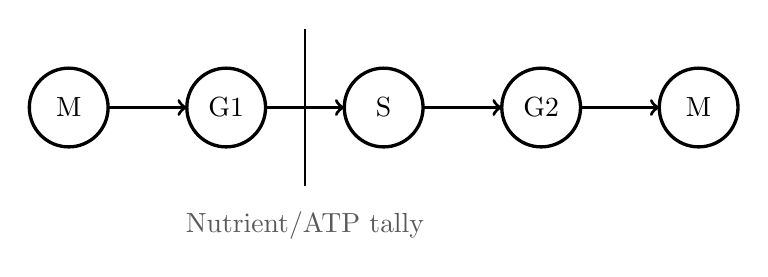
\begin{tikzpicture}

\draw[very thick](-1,0) circle (0.5) node {M};
\draw[very thick, ->] (-1+0.5,0) -- (-1+0.5+1,0);

\draw[very thick](-1+0.5+1+0.5,0) circle (0.5) node {G1};
\draw[very thick, ->] (1.5,0) -- (2.5,0);

\draw[very thick](3,0) circle (0.5) node {S};
\draw[very thick, ->] (3.5,0) -- (4.5,0);

\draw[very thick](5,0) circle (0.5) node {G2};
\draw[very thick, ->] (5.5,0) -- (6.5,0);

\draw[very thick](7,0) circle (0.5) node {M};
 \draw[thick,gray!70!black](2,-1.5) node {Nutrient/ATP tally};
 
\draw[thick] (2,-1) -- (2,1);

\end{tikzpicture}

\subsubsection{"Nutrient \& growth factor" model}
In case where both growth factors and nutrients are included in the model the flow will be as follows :

\vspace{1cm}
\hspace{2cm} 
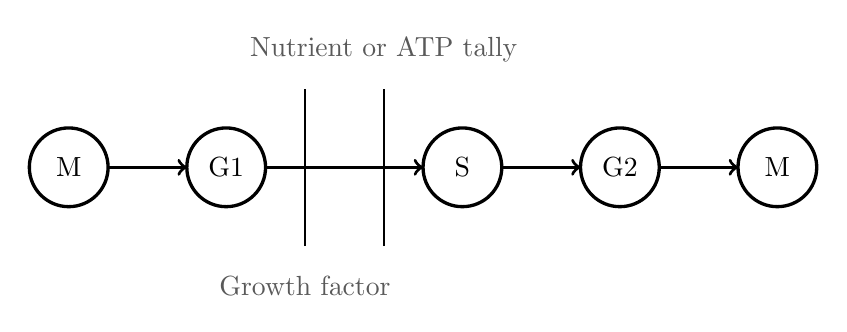
\begin{tikzpicture}

\draw[very thick](-1,0) circle (0.5) node {M};
\draw[very thick, ->] (-0.5,0) -- (0.5,0);

\draw[very thick](1,0) circle (0.5) node {G1};
\draw[very thick, ->] (1.5,0) -- (3.5,0);

\draw[very thick](4,0) circle (0.5) node {S};
\draw[very thick, ->] (4.5,0) -- (5.5,0);

\draw[very thick](6,0) circle (0.5) node {G2};
\draw[very thick, ->] (6.5,0) -- (7.5,0);

\draw[very thick](8,0) circle (0.5) node {M};
 \draw[thick,gray!70!black](2,-1.5) node {Growth factor};
 \draw[thick] (2,-1) -- (2,1);
  \draw[thick,gray!70!black](3,1.5) node {Nutrient or ATP tally};
 \draw[thick] (3,-1) -- (3,1);
\end{tikzpicture}

In the growth factor case the cell goes into G0-phase while in the case of nutrient  depletion, the G1-phase is lengthened until nutrient concentration crosses a given threshold or until the total ATP reaches the right value. In this case, and the previous one, the question of what happens in case nutrients become insufficient before division can be completed is raised and will be answered in the next section.

\subsection{Cell death}
Cell death can be divide into  two different categories. Programmed cell death and non-programmed cell death. Programmed cell death tend to be initiated through signalling pathways. Non-programmed cell death is usually due to a loss of function due to a decline in homeostasis such as a large deviation in redox homeostasis due to mitochondrial damage, a harsh environment, or a loss of ATP. At the level of this model, it would not be worth the effort to try and capture all the subtlty of those cell death variations. However, it will be important to distinguish between apoptosis/autophagy where the cell "disappears" and "necrosis" where it does not. The assumption here will be that two thresholds of ATP can be set. The first threshold, if crossed will lead to non necrotic cell death in a certain amount of time. The second threshold lower than the first will lead to necrosis. This  hypothesis is supported by experimental observations on healthy cells. \cite{Lieberthal1998}\cite{Why1999} \cite{Yee2021} Whether the mutations of apoptotic genes completely shuts it down in favor of necrosis remains to be seen.

In summation, in addition to the quiescence threshold $p_{ATP,q}$, that is only valid in G1 phase before the resriction point, two  other thresholds are defined as $p_{ATP,ap}$ and $p_{ATP,ne}$ with  $p_{ATP,ap} > p_{ATP,ne}$. The precise value if previous study are looked at even a value equivalent to 70\% of the normal one is enough to trigger apoptosis if maintained for long enough and 50 \% triggers necrosis invariably.\cite{Lieberthal1998}

\begin{figure}[ht!]
\vspace{1cm}
\hspace{2cm} 
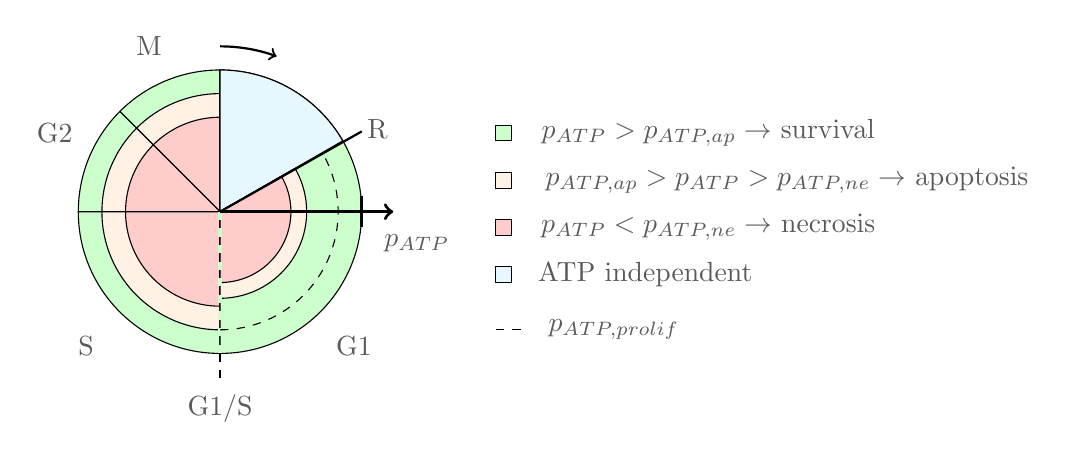
\begin{tikzpicture}


\filldraw[fill=green!20!white, draw=black] (0,0) -- (0mm,18mm) arc (90:135:18mm) -- (0,0);
\filldraw[fill=orange!10!white, draw=black] (0,0) -- (0mm,15mm) arc (90:135:15mm) -- (0,0);
\filldraw[fill=red!20!white, draw=black] (0,0) -- (0mm,12mm) arc (90:135:12mm) -- (0,0);
\draw[thick,gray!70!black](-9mm,21mm) node {M};


\filldraw[fill=green!20!white, draw=black] (0,0) -- (-18*0.707mm,18*0.707mm) arc (135:180:18mm) -- (0,0);
\filldraw[fill=orange!10!white, draw=black] (0,0) -- (-15*0.707mm,15*0.707mm) arc (135:180:15mm) -- (0,0);
\filldraw[fill=red!20!white, draw=black] (0,0) -- (-12*0.707mm,12*0.707mm) arc (135:180:12mm) -- (0,0);
\draw[thick,gray!70!black](-21mm,10mm) node {G2};

\filldraw[fill=green!20!white, draw=black] (0,0) -- (-18mm,0mm) arc (180:270:18mm) -- (0,0);
\filldraw[fill=orange!10!white, draw=black] (0,0) -- (-15mm,0mm) arc (180:270:15mm) -- (0,0);
\filldraw[fill=red!20!white, draw=black] (0,0) -- (-12mm,0mm) arc (180:270:12mm) -- (0,0);
\draw[thick,gray!70!black](-17mm,-17mm) node {S};

\filldraw[fill=green!20!white, draw=black] (0,0) -- (-0mm,-18mm) arc (-90:90:18mm) -- (0,0);
\filldraw[fill=cyan!10!white, draw=black] (0,0) -- (18*0.866mm,18*0.5mm) arc (30:90:18mm) -- (0,0);
\filldraw[fill=orange!10!white, draw=black] (0,0) -- (11*0.866mm,11*0.5mm) arc (30:-90:11mm) -- (0,0);
\filldraw[fill=red!20!white, draw=black] (0,0) -- (9*0.866mm,9*0.5mm) arc (30:-90:9mm) -- (0,0);
\draw[thick,gray!70!black](17mm,-17mm) node {G1};

\draw[draw=green!20!white, dashed,very thick] (0,0) -- (-0mm,-18mm);
\draw[very thick, ->] (0mm,0mm) -- (22mm,0mm);
\draw[very thick] (18mm,2mm) -- (18mm,-2mm);
\draw[thick,gray!70!black](25mm,-4mm) node {$p_{ATP}$};
\draw[draw=black, thick] (0,0) -- (18mm,10.2mm);
\draw[thick,gray!70!black](20mm,10.5mm) node {R};
\draw[draw=black, dashed] (0,-18mm) -- (0 mm,-22mm);
\draw[thick,gray!70!black](0mm,-25mm) node {G1/S};


\draw[thick,->] (0mm,21mm) arc(90:70:21mm);
\draw[dashed] (0mm,-15mm) arc(-90:30:15mm);

%legend
\filldraw[fill=green!20!white, draw=black] (35mm,9mm) rectangle (37mm,11mm);
\draw[thick,gray!70!black](62mm,10mm) node {$p_{ATP}>p_{ATP,ap} \rightarrow$  survival};
\filldraw[fill=orange!10!white, draw=black] (35mm,3mm) rectangle (37mm,5mm);
\draw[thick,gray!70!black](72mm,4mm) node {$p_{ATP,ap}>p_{ATP}>p_{ATP,ne} \rightarrow$  apoptosis};
\filldraw[fill=red!20!white, draw=black] (35mm,-3mm) rectangle (37mm,-1mm);
\draw[thick,gray!70!black](62mm,-2mm) node {$p_{ATP}<p_{ATP,ne} \rightarrow$  necrosis};
\filldraw[fill=cyan!10!white, draw=black] (35mm,-9mm) rectangle (37mm,-7mm);
\draw[thick,gray!70!black](54mm,-8mm) node {ATP independent};
\draw[draw=black, dashed] (35mm,-15mm) -- (39 mm,-15mm);
\draw[thick,gray!70!black](50mm,-15mm) node {$p_{ATP,prolif}$};



%\filldraw[fill=green!20!white, draw=black] (0,0) -- (18mm,0mm) arc (170:210:18mm) -- (0,0);
%\filldraw[fill=red, draw=black] (0,0) -- (12mm,0mm) arc (170:210:12mm) -- (0,0);
\end{tikzpicture}
\caption{Cell fate as a function of ATP production and cell cycle phases \label{cell fate}}
\end{figure}

The cell death and decision making is summarised in figure \ref{cell fate}. from the end mitosis (M) until the restriction point (R) it is assumed ATP production (or nutrient availability) is not critical. The cell can survive these 4 hours through autophagy even if nutrient are depleted. At the restriction point (R), growth factor availability is assessed. If growth factors are present the cell then goes on into the second part of G1 and assess if enough nutrients are present to go into S-phase.

From (R) onward until G1/S, the cell dies if the amount of nutrient prevents it from performing homeostasis, which is not as costly as proliferation. mild depletion will lead to apoptosis while acute depletion will lead to necrosis. After G1/S, since the cell engage active proliferation, the thresholds are raised to reflect the higher ATP consumption overall.

The limit between G1 and S is dashed. This is to signify that cells may arrest growth in G1 if nutrient are not present in sufficient quantity to support proliferation. This behavior is based on the assumption that cells are parcimonious in G1-phase. This means that they will primarily ensure homeostasis and invest surplus into proliferation and preparation of S-phase. This whole reasoning leaves aside a primary aspect of the cell phenotype : migration.

\subsection{The case of cell migration}
In this part, the goal is to attempt to answer three main questions about cell migration in DIPG: 
\begin{itemize}
\item What triggers or stop cell migration ?
\item What is the energetic cost of migration ?
\item How fast is cell migration ?
\item How is it coordinated with proliferation and the cell cycle ? 
\end{itemize}

Definitive answers are not available for most cancer cell lines let alone DIPG whose migration  has seldom been studied from a "biophysical" point of view, as in trying to measure quantitative physical quantities in a large set of conditions. The literature review gives some clues about the behaviour and they will be included in the model with some hypothesis in order to be able to complete the formulation.  In order to find data applicable to the model a first search was conducted for DIPG, then a broader one on Oligodendrocyte precursor cells (OPC), and then other cancer cell lines were also checked to fill in eventual gaps or to confront findings in order to assess the potential variability of a given behavior between cell lines or within a cell line.

\subsubsection{What triggers or stop cell migration ?}
The answer to this question is definitely not trivial. For DIPG cells, observation and preliminary experiments suggest both contact with the right type of matrix and the presence of the right type of growth factors are necessary for cell migration to occur. It should be noted  that under certain culture conditions the cell became adherent monolayers. \cite{Meel2017} (TSM base + 10\% heat inactivated FBS) Elements in the review of Rajasekharan on Oligodendrocyte precursor cells, whose phenotype is close to the studied cell line here, suggest that lack of growth factor inhibits migration. It also states that Fyn pathway may still lead to migration, which is linked to integrin and therefore cell-ECM contact \cite{Rajasekharan2009} DIPG cells (most specifically DIPG-007) also appear to downregulate or underexpress beta-catenin which is linked to cell-cell contact and elevated levels result in reduced migration.\cite{Cockle2015}

It should also be noted that migration will not be treated similarly in the neurosphere and in the chip. Neurospheres do not appear to produce the same type of matrix protein that triggers migration in cells and the abundance of cell-cell contacts may play a role in the inhibition of migration as well.\cite{Campos2004} This is further supported by the fact that spheres grown in non-adherent environment exhibit migration once placed in extracellular matrix scaffolds.\cite{Cockle2015} Experiments from Corning Life Sciences also show that cell can migrate from neurospheres without growth factor if placed in a growth factor depleted envrionment coated with laminin.\cite{Corning} 

\subsubsection{What is the energetic cost of migration ?}
An aspect that has been left out of the discussion so far is the energetic requirement of migration. Estimate suggest that up to 50 \% of ATP requirement could be directed towards migration.\cite{Zanotelli2021} Others studies from the same group showed that denser matrix correlated with higher ATP:ADP ratio in migrating metastatic cells. This means that we have to consider three energy expenses : Homeostasis, Proliferation, and migration. Two hypothesis will be at the foundation of the model on that aspect. Proliferation and migration are equivalent in terms of energy consumption and the repartition of produced ATP during the two remains roughly equal regardless of the amount available energy. For this to be realistic, it is obvious that migration speed and proliferation speed must be slowed down in case of ATP reduced availability.

\begin{figure}[ht!]
\vspace{1cm}
\hspace{4cm} 
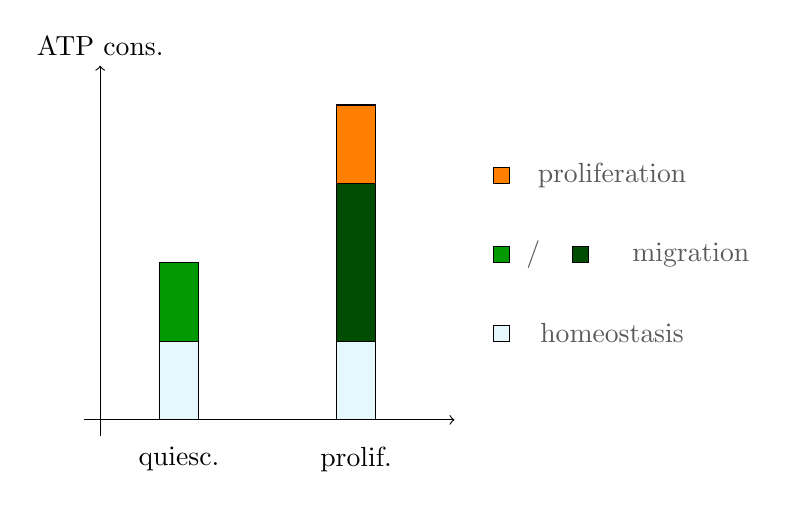
\begin{tikzpicture}[domain=0:4] 
    %\draw[very thin,color=gray] (-0.1,-1.1) grid (3.9,3.9);
    %axes
    \draw[->] (-0.2,0) -- (4.5,0) ; 
    \draw[->] (0,-0.2) -- (0,4.5) node[above] {ATP cons.};
    
    %rectangles
    \filldraw[fill=cyan!10!white,draw=black] (0.75,0) rectangle (1.25,1);
    \filldraw[fill=green!60!black,draw=black] (0.75,1) rectangle (1.25,2);
    \draw (1,-0.5) node {quiesc.};
    
    
    \filldraw[fill=cyan!10!white,draw=black] (3,0) rectangle (3.5,1);
    \filldraw[fill=green!30!black,draw=black] (3,1) rectangle (3.5,3);
    \filldraw[fill=orange,draw=black] (3,3) rectangle (3.5,4);
    \draw (3.25,-0.5) node {prolif.};
    
    \filldraw[fill=green!60!black, draw=black] (5,2) rectangle (5.2,2.2);
	\draw[thick,gray!70!black](5.5,2.1) node {/};
    \filldraw[fill=green!30!black, draw=black] (6,2) rectangle (6.2,2.2);
	\draw[thick,gray!70!black](7.5,2.1) node {migration};
	\filldraw[fill=orange, draw=black] (5,3) rectangle (5.2,3.2);
	\draw[thick,gray!70!black](6.5,3.1) node {proliferation};
	\filldraw[fill=cyan!10!white, draw=black] (5,1) rectangle (5.2,1.2);
	\draw[thick,gray!70!black](6.5,1.1) node {homeostasis};
    
\end{tikzpicture}
\caption{Energy consumption for quiescent and proliferative cells \label{energy}}
\end{figure}

Therefore with cell migration included, the energy consumption of a cell is taken as shown in figure \ref{energy}. In the quiescent state, energy is evenly split between homeostasis and slow migration. If ATP production capacity falls the cell will prioritize homeostasis and migration will be slow gradually until it reaches zero. If ATP production decreases further then cell death may occur. For proliferating cells, migration is faster and more energy consuming than in quiescent cells. Biosynsthesis also consumes a lot energy and homeostasis is considered to be roughly the same. However, it is important to note after G1/S checkpoint, the threshold for survival will be considered to be higher (see fig.\ref{cell fate}). The reason is that the commitment to division cannot be halted the way it can be in G1. It is therefore considered that the proliferation energy cost is necessary for survival and thus the only "dispensable" energy expense becomes migration.  
 

\subsubsection{How fast is cell migration ?}
Data on oligodendrocyte precursor cells  gave a mean velocity of 10 \textmu m/h with maximal value of 120 \textmu m/h.\cite{Happel2013} Other measurements on OPCs yielded values between 10 \textmu m/h and 20 \textmu m/h. and measurement on U251 glioma cells yielded of 30 \textmu m/h.\cite{Piltti2017}   

Following up on previous knowledge, it is assumed that migration and proliferation will slow down in similar proportion. They will slow down until the apoptosis threshold is reached.

\begin{figure}[ht!]
\vspace{1cm}
\hspace{4cm} 
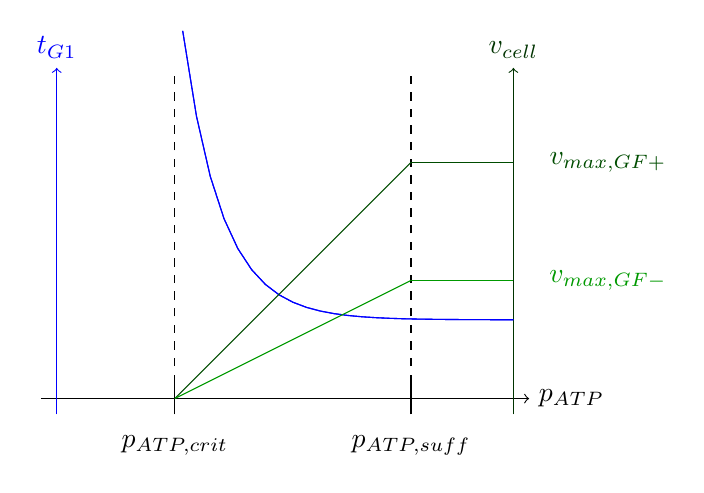
\begin{tikzpicture}[domain=0:4] 
    %\draw[very thin,color=gray] (-0.1,-1.1) grid (3.9,3.9);
    %axes
    \draw[->] (-1.7,0) -- (4.5,0) node[right] {$p_{ATP}$}; 
    \draw[->,color=green!20!black] (4.3,-0.2) -- (4.3,4.2) node[above] {$v_{cell}$};
    \draw[->,color=blue] (-1.5,-0.2) -- (-1.5,4.2) node[above] {$t_{G1}$};
    
    %ticks
     \draw[-] (0,-0.2) -- (0,0.2);
     \draw (0,-0.6) node {$p_{ATP,crit}$};
     \draw[-] (3,-0.2) -- (3,0.2);
     \draw (3,-0.6) node {$p_{ATP,suff}$};
     
     %lines
     \draw[dashed] (0,0.2) -- (0,4.2);
     \draw[dashed] (3,0.2) -- (3,4.2);
     
      \draw[domain=0.1:4.3,color=blue] plot (\x,{exp(-2*\x+1.5)+1});
      \draw[domain=0.1:4.3,color=blue] plot (\x,{exp(-2*\x+1.5)+1});
      \draw[domain=0:3,color=green!30!black] plot (\x,\x);
      \draw[domain=3:4.3,color=green!30!black] plot (\x,3);
      \draw[color=green!30!black] (5.5,3) node {$v_{max,GF+}$};
      \draw[domain=0:3,color=green!60!black] plot (\x,0.5*\x);
      \draw[domain=3:4.3,color=green!60!black] plot (\x,1.5);
      \draw[color=green!60!black] (5.5,1.5) node {$v_{max,GF-}$};
  \end{tikzpicture}
  \caption{Relation between ATP production, cell migration speed and G1 phase length \label{vcell}}
\end{figure}

As shown in figure \ref{vcell} the relation is in fact opposite. G1 will lengthen until the minimal threshold for survival is crossed. Cell migration speed will increase with ATP production until a maximum value which will depend on the presence of growth factors. If growth factors are abundant, maximum migration speed will be higher to reflect how growth factors promotes migration (but are not necessary for it to occur).

Though it was represented as a linear increase in figure \ref{vcell}, the speed slope will most likely be a sum of heaviside function due to the coarse (cell-level) spatial discretization of the model.

\subsubsection{How is it coordinated with proliferation and the cell cycle ?}
A timelapse of Huang on Oligodendrocyte precursor cells shows that OPC progressively stop migrating stop their migration 1 to 2 hours before dividing and then resume. Suggesting that migration can basically occur at anytime that is not division.\cite{Huang2020} Data gathered on other cell types showed that at a given time up to 80 \% of migrating cells are in G1 or S-phase while the rest are in G2.\cite{Alhashem2022} There is also evidence that cells in G0 phase migrate too for certain cell types.\cite{Lamb2014}

\begin{figure}[ht!]
\vspace{1cm}
\hspace{4cm} 
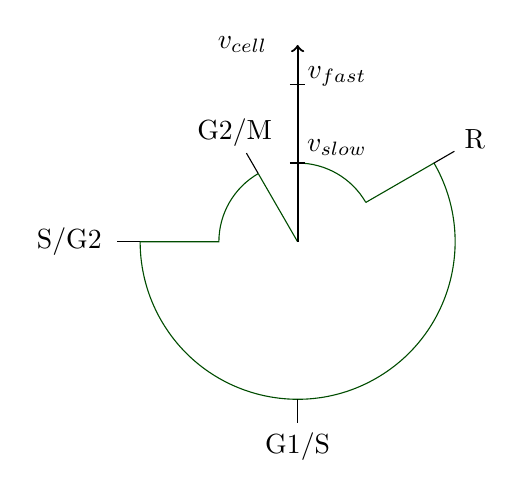
\begin{tikzpicture}
%circle & arcs
\draw[draw=green!30!black] (90:0) -- (90:1) arc (90:30:1);
\draw[draw=green!30!black] (30:1) -- (30:2) arc (30:-180:2);
\draw[draw=green!30!black] (-180:2) -- (-180:1) arc (-180:-240:1);
\draw[draw=green!30!black] (-240:1) -- (-240:0);

%axes & lines
\draw[->,color=black, thick] (90:0) -- (90:2.5) ;
\draw[color=black] (-0.7,2.5) node {$v_{cell}$};
\draw[color=black] (-0.1,1) -- (0.1,1);
\draw[color=black] (0.5,1.2) node {$v_{slow}$};
\draw[color=black] (-0.1,2) -- (0.1,2);
\draw[color=black] (0.5,2.1) node {$v_{fast}$};
\draw[color=black] (90:-2) -- (90:-2.3) node[below] {G1/S};
\draw[color=black] (30:2) -- (30:2.3);
\draw[color=black] (30:2.6) node{R};
\draw[color=black] (180:2) -- (180:2.3);
\draw[color=black] (180:2.9) node{S/G2};
\draw[color=black] (120:1) -- (120:1.3);
\draw[color=black] (120:1.6) node{G2/M};
\end{tikzpicture}
\caption{Relationship between cell cycle phase and migration speed for proliferating cells \label{vcycle}}
\end{figure}

For proliferating cells, the migration speed will depend on the cell cycle phase as shown in figure \ref{vcycle}. This would be the ideal, most realistic situation. Though this may be simplified into only fast and slow phases  for the sake of simplicity (the stop phase for division would be removed). Quiescent cells can only move at speed between $v_{slow}$ and 0 as they are not stimulated by growth factors.

\subsubsection{Coupling between migration and proliferation ?}
A final question is how the proliferating cells divide their energy between migration and proliferation when ATP reserves drop because of lack of nutrients. The answer to this question is not straightforward as migration and proliferation are not completely coupled. For example, Flubendazole can induce G2/M cell cycle arrest with no impact on migration\cite{Zhou2018}. Cell cycle arrest induced through the YAP signalling pathway also inhibits migration in glioblastoma cells.\cite{Wang2023} Propofol has been shown to impact both proliferation and migration in glioma cells.\cite{Cheng2022} Silencing of the HIWI gene also reduced both proliferation (by inducing cell cycle arrest and apoptosis) and reduced cell migration.\cite{WangX2014} Cation channel have also been shown to impact proliferation and migration likewise.\cite{Rooj2011} Ginkgolic acid is also reported to inhibits cell migration and proliferation in glioblastoma.\cite{Li2021} Eupatilin has also been shown to disrupt both migration and proliferation.\cite{Fei2019} Interestingly for head and neck cancer, TGF-$\beta$ in head and neck cancer generates population of arrested cells  with high motility.\cite{Takahashi2022} as TGF-$\beta$ is also the pathway involved in cell cycle arrest modelling it obviously is interesting to know how it can impact migration in glioma specifically. it is reported that TGF-$\beta$ expression may enhance glioma migration.\cite{Han2015} If put together with Foster's interpretation, the hypothesis can then be that TGF-$\beta$ expression due to lack of nutrients inhibits cell cycle progression but promotes cell migration\cite{Foster2010} Uckun and collaborators have shown that in the specific case of DIPG patients, overexpression correlated with poorer prognosis in terms of invasion suggesting that expression TGF-$\beta$ may indeed promote invasion and possibly migration.\cite{Uckun2023} The whole picture is of course more complex and invovlves several pathways but it would be difficult to account for all of them. in conclusion, it will be considered that the TGF-$\beta$ pathway may trigger/enhance migration in harsh environment (typically mild hypoxia). it should however be noted that Kim and collaborators reported that TGF-$\beta$ in cancer cells has little regulatory effect on proliferation. The simplest way would thus be to considered migration and proliferation to be regulated similarly by nutrients.

\subsection{The differences between neurospheres and the chip}
One of the reasons 3D culture models became a source of interest for the scientific community especially in cancer research is due to the impact of mechanics.\cite{Romani2020} Pathways like Wnt, NOTCH and YAP/TAZ, are famously deregulated in cancer. This interplay between mechanics and proliferation, migration  and general cell physiology is also present in DIPG cells. Interestingly observation suggest they are not sensitive to contact inhibition. Nonetheless the very different nature of the two configuration should be mentioned.

\subsubsection{Cell-cell vs cell-matrix}
In the case, of neurosphere, cells have a lot of cell-cell contact which do not involve exactly the same pathways as cell-matrix contacts. This has an impact on the metabolic behavior of a given cell line. For example, it has been reported that ECM detachment from a Hyaluronic acid matrix increased glucose metabolism in various cell lines including U-87 glioma cell line.\cite{Sullivan2018} It has also been shown that stiffer environment promotes glioma aggressiveness through PIEZO1.\cite{ChenX2018} Most literature found on this subject seem to present a rather coherent picture : Stiff environment tend to promote proliferation, glyoclysis and migration. \cite{Chen2021}\cite{Barnes2017}

Jiang and collaborators also reported on lung cancer cells that oxygen consumption increased in the monolayer situation compared to the spheroid. This is the first quantitative data we found on that matter and they show OCR to be reduced by two thirds in spheroid compared to monolayers.\cite{Jiang2016}

It should however be noted that even in the sphere configuration, the cells most likely produce some ECM molecules. In rat or mouse neurosphere, Laminins and fibronectins are produced by cells in the neurosphere, with Fibronectin being present all across the sphere while laminin is mostly present at the edge.\cite{Campos2004}

\subsubsection{Access to metabolite}
In the chip configuration, metabolites and nutrients are supplied radially to cell/matrix ensemble. Cells not having too many cell-cell contacts it can be assumed that the matrix will be the limiting diffusion medium and that no significant tortuosity impacts mobility of different molecules, except for oxygen which crosses membranes anyway. 

For glucose and glutamine, the impact is roughly the same. The neurosphere compaction leads to a high tortuosity and therefore a reduced diffusion coefficient in addition of the consumption term. The depletion layer is therefore expected to be radially thinner than in the sphere configuration. However a main question that should be adressed is what the matrix in the sphere is made of and how it impacts diffusion compared to the hyaluronic acid/matrigel mixture of the chip configuration.

As literature review for growth factors was conducted, evidence accumulated that modelling such a process accurately would prove extremely difficult. This will be develop in the next subsection

\subsection{The growth factor question}
Growth factor were slated for inclusion in the model from early on due to their assumed role in the passage of the restriction point R, and promotion of cell proliferation and cell migration.\cite{Nabil2021}\cite{Rajasekharan2009}\cite{Bauer2004}

However several problems makes the realistic inclusion of growth factor in the model extremely challenging. First of all, there is a general scarcity of data on diffusivity and consumption rate. Rough estimates on diffusivity and consumption rate could be found based on experimental data found in the literature. However, these lead to a more qualitative problem.

Growth factors in solution are reported to have short half-lives (hours at most).\cite{Ren2020}\cite{Teixeira2020} For this reason, in vitro and in vivo growth factors tend to be attached to larger molecules which stabilises them. These molecules are typically molecules of the ECM. The interactions between cells and growth factors thus become a function of the attached molecules, not only through their physical and chemical properties, but also through their interactions with the cell membrane.\cite{Teixeira2020}\cite{ChenJW2018} 

Even assuming that the previous interactions are completely sorted out, the question of spatial and temporal aspects of internalisation of the "growth factor-receptor" complex would still need to be adressed. For example, attachement to a large protein may prevent internalisation altogether as long as the large ECM protein is not dissociated from the complex possibly leading to continuous promitotic signalling, but also to the  prolonged unavailability of the receptor. On the contrary, internalised GFR complex may be dissociated very quickly leaving the receptor open to return to the membrane and bind to a new growth factor.\cite{Ren2020}\cite{Teixeira2020}

All the previous fact lead to the conclusion that there is simply not enough knowledge on growth factors as is for them to be included in the model without massive and uncheckable hypothesis having to be made.

\subsubsection{The migration question}
The question of migration in the chip is rather straightforward. It will be considered to be triggered by the cell-matrix contact, and therefore present by default in the chip configuration. It may be hampered by lack of nutrient, or on the contrary increased by "moderate" hypoxia However, quiescence does not equate with arrested migration. Since hypoxia now becomes a major factor in the model, its impact on migration should also be assessed. Several studies make a direct link between the upregulation of HIF-1$\alpha$ and enhanced migration.\cite{Joseph2015}\cite{Velasquez2019}\cite{Eckerich2007} 

It is thus important to know or at least estimate the level at which the HIF-1 induced migration increase will result in increased migration. In her review, McKeown reports that the oxygen level for HeLa cells inducing maximal HIF-1$\alpha$ response was 0.5\% (0.00375 mM) with a half response obtained 1.5-2\% (0.01125-0.015 mM) and a low expression at 4\%.\cite{McKeown2014}

\subsection{Hypoxia-induced arrest/quiescence}
As explained in the previous subsection, growth factors will be left out of the new model even though they were intially included. The big question thus becomes how is the restriction point passage decided ? Or, more braodly, what induces cell quiescence ?

Fortunately, a recent study outlines the answer to that question.\cite{Nabil2021} Glucose is also reported to possibly induce quiescence. However, the cited study never removes glucose or inhibits glucose transporter without removing serum as well, which prevents from establishing firmly the role on glucose in the phenomenon.\cite{Hu2011}
However several reported studies establish how hypoxia leads cells to a quiescent state either through exposition to an oxygen depleted environment or through a chemical used to emulate this situation.\cite{Nabil2021} One of those study observed the effect hypoxia on monolayer and 3D cultures of MCF-7 cells. Hypoxia (0.1\% level) induced drasti augmentation of quiescent cell numbers and practically stop growth in the monolayer culture with a reaction time of less than 2 days.\cite{Lee2018}

Therefore, severe hypoxia will be selected as the new criterion for the passage of the restriction point. This however raises the question of the value for the threshold, as it might be higher than 0.1\%(0.0075 mM). McKeown's review on the subject supports that a value of 1\% (0.075 mM)  is realistic as a threshold where the effect of hypoxia are already felt. It is also explained that hypoxia can lead to tumor cell death if the level falls below 0.01\% (0.0075 mM).\cite{McKeown2014} These are the values that will be used in the model.

As for growth factor, exiting the cell cycle is only considered possible in the 4 hours  after mitosis. Cells being starved of oxygen past this point will remain in arrested G1 or undergo cell death. or not

It should be noted that CoCl2 at low (100 µM) concentration seem to stimulate proliferation rather than stop it and that the significant slowdown in growth observed by Lee et al. at 100 \textmu M was only observed at 150 \textmu  M by Rana and collaborators.\cite{Lee2018}\cite{Rana2019} While this quantitative discrepancy on otherwise identical cell line raises questions it nonetheless point towards the same qualitative conclusion : Mild hypoxia stimulates growth while acute hypoxia stops it which is also observed in other studies.\cite{Wigerup2016}\cite{Li2009} Migration seems to work the same way.\cite{Bhagat2016}


\subsection{Quiescence, Arrested G1, growth factors and nutrients}
To know whether cell are quiescent or in state of cell cycle arrest is considered to be an important question for our model. Our first intuition, following textbooks treating broad biology subjects was that cells had a restriction point in G1, whose passage was modulated solely by the presence of growth factor.\cite{Cooper2006} Howevern as literature on cancer cells was being surveyed, a more complex image of the truth emerged.

A good starting point for this question in literature is the review of Nik Nabil and collaborators.\cite{Nabil2021} In their review, they explicitly state that quiescent cells are non-proliferating (Ki-67 negative) and that their passage into quiescence can be modulated by several factors other than serum inclusion in culture medium. It has been shown that acute hypoxia (0.1\%) led to a majority of cancer cells going quiescent on breast cancer cultures.\cite{Lee2018} Glucose starvation with maintained supply of serum have also resulted in a higher proportion of quiescent cells in glioblastoma cells.\cite{WangL2018} 

Another important point is whether G0 cells should be distinguished from arrested G1 cells. A study on the dynamics of Ki67 seems to suggest that no difference should be made between G0 and arrested G1\cite{Miller2018} Other studies also present G0/G1 cells indistinctly.\cite{Jiang1998}\cite{Song2018} Another study also presents arrested G1 cells as Ki-67 negative which is the criterion for the definition of G0 cells.\cite{Sobecki2017} However, the way the restriction point and nutrient checkpoint are presented in the study of Foster seem to suggest a difference between G0 and arrested G1. The main difference pointed here seemingly being the time difference in recovery between serum deprivation and amino acid deprivation observed by Yen and Pardee.\cite{Yen1978} Indeed amino acid deprived cells recovered in 2 hours while serum deprived cells took 12 hours to progress to S. This, seem to be understood by many as evidence of different quiescent state.

Foster and colleagues point out, however, that the mTOR pathway that is supposed to be activated in presence of sufficient nutrient may also be sensitive to growth factors which is also stated by in mammals. The previous fact is also stated in other studies.\cite{Fingar2004} This blurs the line of separation between nutrient action and growth factor action. This however explains how nutrient starvation may results in cell quiescence even in presence of sufficient growth factors.

In fact, none of the previously cited studies ever present G0 and arrested G1 as explicitly different. Some use only the term arrested G1 and other use both G0 and arrested G1. However, this leaves open the question of what happens when G1 cell cycle arrest is induced after the restriction point. In their article from 2000, Donovan and Slingerland state the following: "Cells are sensitive to TGF-$\beta$ during a discrete period in early G1 phase, until they reach a 'restriction point' 6-10 h after G0 release [47,48]. When TGF-$\beta$ is added after this critical time point, cells complete the cell cycle but arrest during the subsequent G1 phase." Suggesting that once the restriction point is passed cells will go through the entire cell cycle.\cite{Donovan2000} This suggest that an arrested state that is not the growth factor meidated G0 exists and may maintain itself as long as the second checkpoint depending on TGF-$\beta$ and related to nutrient is not passed. 

The broader picture seem to be that of a continuum of possible quiescent state. The deepest quiescent state being obtained by complete deprivation of growth factor. The cell then stops until growth factors are replenished and takes between 6 and 10 h  to get to the 2nd checkpoint where nutrient availability is checked. This other quiescent is a priori different from G0 from a molecular point of view as it takes less time to exit and it is triggered by a different pathway. it this second checkpoint, if passed that leads to full commitment to mitosis. Therefore, in our model a clear difference will be made between arrested G1 and G0. However, this distinction will remain artificial as growth factor dynamics have yet to be elucidated. An important thing to note is that in both case it is probable that cells are Ki-67 negative.

\section{First studies}
In the previous sections we outlined broad aspects of the model which will hopefully be included in broader general hybrid model which  may respond realistically to environmental cues, recapitulate metabolic plasticity of cancer cells and be able to yield interesting data on cell growth dynamics first in normal situation and then potentially in situation where drugs and/or radiation will be applied to the system.

One of the main difficulties is the various timescales that are involved in the system and that would force a complete model to have small space and time step while also covering large duration. A prime example is the case of oxygen. if the model space scale is that of a cell ($\approx$  15 \textmu m), the diffusion values for oxygen in tissue ($\approx$ 100000 \textmu m/s) means that the time step needs to be approximately 1/1000 of a minutes. Keeping in mind that cell cycle is between 18h and 24h, any spatially extended system can become very computationally costly. Even though the authors intend to at some point tackle the full model, it is considered more efficient to break some of the question into bite-sized pieces of more manageable modelling problems. To illustrate this approach, the case of  the oxygen within the chip will be treated thoroughly in the following subsection.

\subsection{Establishment of hypoxia, and cell response} 
Before modelling a full cell cycle it is interesting to know what the nutritional landscape of the cells will be. Here, the focus will be placed firmly on the chip situation and the oxygen supply as preliminary calculation showed that due to consumption and diffusion other nutrients will not undergo shortage before at least 24h even at the center of the chip.

\subsubsection{Hypotheses and configuration}
The model is designed to represent the chip configuration. In order to save computational resources only the median layer of the 750 \textmu m system will be represented as it is assumed that translational invariance along the z-axis is valid in the system.

The geometry of the model is as follows : the modelled zone is divided into the fluid/supply area and the matrix/cell region. The entire square grid is 5400 \textmu m by 5400 \textmu m. A 4500 \textmu m-diamter circular region in which each pixel represents either a cell or matrix. Cells are able to progress within the matrix by hopping from pixel to pixel. The specifics and quantitative aspects will be discussed further. 

\begin{center}
	\begin{tabular}{ |p{22mm}|p{15mm}|p{15mm}| }
		\hline
		\textbf{Parameters} & Value & Ref.  \\ 
		\hline
		\textbf{$D_Ox$ (\textmu m)} & 100000 \textmu / min & \cite{Hober1947} \\
		\textbf{$q_{O,max}$ (\textmu m)} & 2 mM/min/cell & \cite{Ruas2018}\cite{Mbah2022}\cite{Shen2020}\\
				\textbf{$[0]_{O}$ (\textmu m)} & 0.15 mM & Experimental conditions
	\end{tabular}
\end{center}

The value for OCR is not  to be adjusted as we consider that the contact with the HA/matrigel scaffold produces similar effect to the laminin-coated surfaces used by Shen, Mbah and their collaborators to assess the OCR with the seahorse experiments.

As will be shown further migration is not included in the model yet as the modelling time will typically be of the order of 60 mn. s On such a short time even the most active cells would only jump one site and therefore migration cannot at this timescale provoke any serious reorganizing of the system.

\subsubsection{First results}
In the first case, we model the case where oxygen supply in supposedly constantly renewed by supply of oxygenated medium. 

\begin{figure}[ht!]
	\begin{subfigure}{0.45\textwidth}
	\centering
	\includegraphics[scale=0.425]{/home/antony/Documents/Post-doc/test_fortran/plots/GO/cfsys2DGO_O_conf6.pdf}
	\caption{ \label{O_conf5_ct}}
	\end{subfigure}
	~~
	\begin{subfigure}{0.45\textwidth}
	\includegraphics[scale=0.425]{/home/antony/Documents/Post-doc/test_fortran/plots/GO/cfsys2DGO_Ot_conf6.pdf}
		\caption{ \label{Ot_conf5}}
	\end{subfigure}
	\caption{Contour map of oxygen concentration with pellet outlined in red  \label{Oconf6} for a cell concentration of 10 000 cell per \textmu L }
\end{figure}
What can be seen in figure \ref{Oconf6} is that the oxygen concentration stabilizes in less than 10 minutes in the whole system and that concentration at the core of the chip falls to zero.

Now to push the analysis further we seek the assess the impact of this physical reality on the behavior of cells in the chip. Following the review of McKeown, acute hypoxia (expression of HIF1-$\alpha$ start at about 2 \% (0.015 mM) and ranges down to 0.1 \% (0.00075 mM) without immediate cell death.\cite{McKeown2014} literature review supports that cells subjected to that level of acute hypoxia will proliferate less and that this proliferation will rest mostly on glycolysis.\cite{Wigerup2016}\cite{Fuchs2020}\cite{Jiang2016}

\begin{figure}
	\centering
	\includegraphics[scale=0.5]{/home/antony/Documents/Post-doc/test_fortran/plots/GO/cfsys2DGO_O_ctr_conf6.pdf}
	\caption{ Contour plot of oxygen concentration in the chip configuration with constant supply \label{O_conf6_ct}}
\end{figure}

In figure \ref{O_conf6_ct}, the data from the previous figure is reploted in contours and rescaled in order to bring up the hypoxic area. The hypoxic area start when oxygen concentration falls below 2\%. In the model, this is shown to happen at 1 mm depth. There is also 100-200 \textmu m zone at the center where the concentration falls to zero (or at least at approximately 0.1\%) in the range of acute hypoxia which we assume will stop growth.

\begin{figure}[ht!]
\vspace{1cm}
\hspace{4cm} 
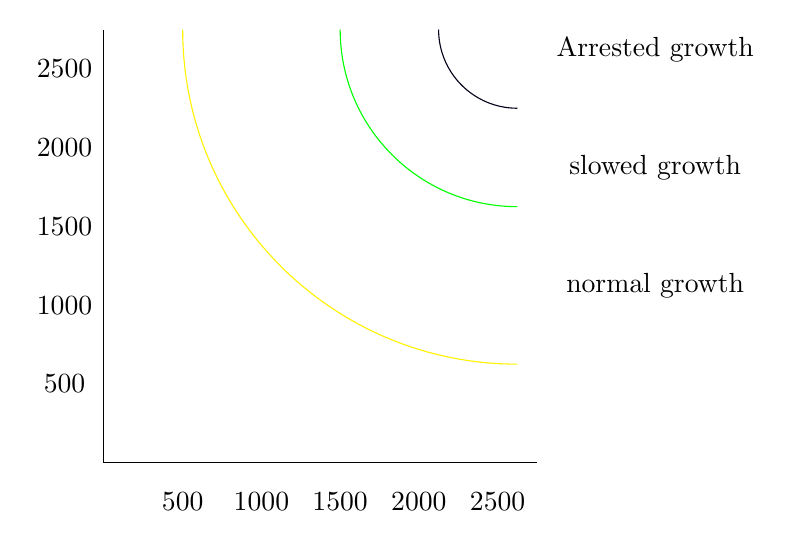
\begin{tikzpicture}
	\draw(0,0)--(0,5.5);
	\draw(-0.5,1) node {500};
	\draw(-0.5,2) node {1000};
	\draw(-0.5,3) node {1500};
	\draw(-0.5,4) node {2000};
	\draw(-0.5,5) node {2500};
	
	\draw(0,0)--(5.5,0);
	\draw(1,-0.5) node {500};
	\draw(2,-0.5) node {1000};
	\draw(3,-0.5) node {1500};
	\draw(4,-0.5) node {2000};
	\draw(5,-0.5) node {2500};
	
	\draw[color=blue!10!black](4.25,5.5) arc(180:270:1);
	\draw(7,5.25) node {Arrested growth};
	
	\draw[color=green](3,5.5) arc(180:270:2.25);
	\draw(7,3.75) node {slowed growth};
	
	\draw[color=yellow](1,5.5) arc(180:270:4.25);
	\draw(7,2.25) node {normal growth};

\end{tikzpicture}
\caption{Estimated behavior for different zones of the chip  \label{sum_O}}
\end{figure}

An interesting question is to know how to different zones will be distributed after 24h in a system where no fresh oxygen is supplied. Of course, the full calculation would require to account for migration and to a certain number of cells having undergone division. But as a first approximation it will be assumed that the cell concentration has not changed after 24h to get a first idea. 

\begin{figure}[ht!]
	\begin{subfigure}{0.45\textwidth}
	\centering
	\includegraphics[scale=0.425]{/home/antony/Documents/Post-doc/test_fortran/plots/depGO3/cfsys2DdepGO3_O_conf6.pdf}
	\caption{ \label{O_conf5_ct}}
	\end{subfigure}
	~~
	\begin{subfigure}{0.45\textwidth}
	\includegraphics[scale=0.425]{/home/antony/Documents/Post-doc/test_fortran/plots/depGO3/cfsys2DdepGO3_Ot_conf6.pdf}
		\caption{ \label{Ot_conf5}}
	\end{subfigure}
	\caption{Map of oxygen concentration with pellet outlined in red  \label{Oconf6} for a cell concentration of 10 000 cell per \textmu L }
\end{figure}

The first results shows that without constant supply the oxygen would drop to zero in less than 2 hours triggering generalized growth arrest across the whole chip. This might explain why cells stop migrating and proliferating after a time.


 
 
\section*{to be treated}

OCR decreased by 2/3rds in spheroid compared to monolayer

%https://www.ncbi.nlm.nih.gov/books/NBK9876/ garder ça pour plus tard (grosse ref sur les cellules eukaryotes



1.      Round-table flash presentation (background and interests)

2.      Basics of the project :

-        OxyMEMS origins : a tumor-on-a-chip to better understand the resistance of DIPGs to therapies (Samuel Meignan) 

-        Proofs-of-Principle : generating hypoxic tumors with gradients of cell density (Lisa Terrassoux) 

-        Connecting Tumor-on-chips to Blood Brain Barrier (Salimata Bacari, Anthony Treizebre)

-        Mathematical models for cancer cell growth, oxygen consumption… in spheroids (Fabrizio Cleri) 

-        Description of the Work Packages proposed in the INCa project (Alessandro Furlan)

3.      Biophysical questions to be addressed / how to answer them (experimentally and theoretically) ?

-        Drug distribution, nanoparticle diffusion, interstitial pressure

-        Oxygenation : oxygen sensors (molecular probes, microelectrodes, Oxnano technology … ?)

-        Reactive Oxygen Species/ Metabolism/Radioresistance

-        Matrix rigidity and mecanotransduction (Traction Force Microscopy), fiber reorientation

if you do wide field, you need to slice or you're not getting images at the core...?


**Cell kinetic characteristics in different parts of multicellular spheroids of human origin KEEP THIS

https://faseb.onlinelibrary.wiley.com/doi/epdf/10.1096/fj.02-0352rev discute cette histoire de G1 et G0 mais je comprends pas vraiment.
\newpage
\bibliographystyle{unsrt}
\bibliography{biblio_synthese}
\end{document}
% Si 15 mM de glucose -> 50 pmol initialement dispo 
% si les consos sont justes on est entre 0.6 et 1.2 fmol/min pour une cellule de 15 µm de diam 
% donc normalement ça met 400 à 800 mn à se vider !